% Generated by tools/supplementary/make_supplementary.py (supp-public-1.0 (2026-10-21)). Do not edit by hand; edit the generator.
\documentclass[10pt,a4paper]{article}
\usepackage[T1]{fontenc}
\usepackage[utf8]{inputenc}
\usepackage[margin=2.0cm]{geometry}
\usepackage{booktabs,longtable,float,graphicx}
\usepackage[hyphens]{url}
\usepackage{hyperref}
\title{Supplementary Material\\[4pt]\large Uncertainty Evaluation to Support Safety of the Intended Functionality Analysis for Determining the Applicability of Performance Targets Across Triggering Conditions in ML-Based LiDAR Object Detection}
\author{Milin Patel \and Rolf Jung}
\date{}
\begin{document}
\maketitle
\tableofcontents

\section{How to read this document}\label{sec:intro}
This document lists the recorded results behind the paper in full: the outcome of every cell on every split, the intervals and retention behind each outcome, the counts behind the KITTI rule, the division by recorded sequence, the predictions fixed in advance, the selection of the frames shown in Fig.~1 and the post-hoc analyses. Nothing in it is recomputed: \path{tools/supplementary/make_supplementary.py} reads every number from a file of the repository and lists it with file, line or row, and column in \path{docs/supplementary/supplementary_sources.csv}; its option \texttt{-{}-check} re-reads each listed value and compares it with the print.

\paragraph{One cell.} A threshold $\tau_c$ is selected in the \emph{condition of selection} $c$ (columns \texttt{established} or \texttt{source} in the files) on the selection part, at limit $\alpha$ and error probability $\delta=0.05$, and tested on the test part of the \emph{condition of use} $c'$ (\texttt{applied} or \texttt{target}). The one-sided Hoeffding--Bentkus bounds $L$ and $U$ of the false acceptance proportion (FAP) $A_{c'}(\tau_c)$, each at $\delta/2$, decide the outcome: \textbf{A} applicable ($U\le\alpha$), \textbf{N} not applicable ($L>\alpha$), \textbf{?} not determined (otherwise), \textbf{-} no threshold selected in $c$. A code string such as \texttt{A??NN} gives the outcome on splits 0 to 4 from left to right. A cell with $c'=c$ tests a threshold in its own condition of selection and checks the selection; a cell with $c'\ne c$ is a \emph{transfer}.

\paragraph{Limits.} The target limits $10^{-2}$, $10^{-3}$ and $10^{-4}$ were fixed before the first run. The limits 0.05 and 0.1 were fixed at the same time as exploratory limits, to show which outcomes the data can decide; they are not safety targets. No threshold could be selected at $10^{-3}$ or $10^{-4}$ in any condition.

\paragraph{Terms and files.} The repository's \path{docs/glossary.md} defines every term and maps it to the column names of the files, which keep the names they were written with (for example \texttt{applies} for applicable, \texttt{eval} for the test part). Run names m1 to m8 identify the scripts in \path{experiments/} and the folders in \path{results/}. Distance conditions are assigned per detection (boundary: median distance of the car detections in the grid part); weather and dataset are assigned per frame. KITTI results apply the KITTI rule unless stated otherwise.

\section{Condition classes}\label{sec:classes}
Each condition is represented by a class of frames or detections in which one process acts on the point cloud. Neither dataset labels classes C3 and C4, and they are not measured.

{\scriptsize
\begin{longtable}{p{0.8cm}p{3.0cm}p{6.2cm}p{3.4cm}}
\caption{Condition classes, defined by the process acting on the point cloud.}\label{tab:classes}\\
\toprule
class & process & effect on detections & measured \\
\midrule
\endfirsthead
\toprule
class & process & effect on detections & measured \\
\midrule
\endhead
\bottomrule
\endfoot
C1 & airborne scatterers & returns without a surface behind them; fewer distant returns & with C2, as recorded rain \\
C2 & surface water, spray & non-rigid clusters; fewer ground returns & with C1, as recorded rain \\
C3 & vehicle-like structure & consistent geometry where no vehicle is & no \\
C4 & occlusion & partial evidence on a present object & no \\
C5 & distance & fewer returns per object & both datasets \\
\end{longtable}
}

\section{Per-split outcome tables}\label{sec:outcomes}
Each line is one cell of an applicability matrix: the threshold selected in one condition (\emph{sel.}, condition of selection) tested in the condition of use (\emph{use}) at limit $\alpha$. The code string gives the outcome per split, seeds 0 to 4 from left to right: \texttt{A} applicable, \texttt{N} not applicable, \texttt{?} not determined, \texttt{-} no threshold selected. The detailed tables give, per split with a threshold, the threshold $\tau$, the false acceptance proportion $\hat A$ with its two-sided HB interval ($\delta=0.05$) and the retention $\hat R$, as recorded. Limits $10^{-2}$, $10^{-3}$, $10^{-4}$ are the target limits; 0.05 and 0.1 are exploratory limits.

\subsection{nuScenes, distance (m3)}
Source: \path{results/m3_nuscenes_distance/matrix_all_variants.csv}. Variants: overlap setting (IoU 0.5), object set (car; vehicles), cut quantile of car range in the grid part (0.25, 0.5, 0.75). The primary variant is car, cut quantile 0.5.

{\scriptsize
\begin{longtable}{lllllll}
\caption{nuScenes distance (m3), all variants: outcome per split.}\label{tab:m3c}\\
\toprule
objects & cut q. & ind. & $\alpha$ & sel. & use & seeds 0--4 \\
\midrule
\endfirsthead
\toprule
objects & cut q. & ind. & $\alpha$ & sel. & use & seeds 0--4 \\
\midrule
\endhead
\bottomrule
\endfoot
car & 0.25 & u\_e & $10^{-2}$ & far & far & \texttt{?A?AA} \\
car & 0.25 & u\_e & $10^{-2}$ & far & near & \texttt{?????} \\
car & 0.25 & u\_e & $10^{-2}$ & near & far & \texttt{AAAAA} \\
car & 0.25 & u\_e & $10^{-2}$ & near & near & \texttt{AAAA?} \\
car & 0.25 & u\_e & $10^{-3}$ & far & far & \texttt{-----} \\
car & 0.25 & u\_e & $10^{-3}$ & far & near & \texttt{-----} \\
car & 0.25 & u\_e & $10^{-3}$ & near & far & \texttt{-----} \\
car & 0.25 & u\_e & $10^{-3}$ & near & near & \texttt{-----} \\
car & 0.25 & u\_e & $10^{-4}$ & far & far & \texttt{-----} \\
car & 0.25 & u\_e & $10^{-4}$ & far & near & \texttt{-----} \\
car & 0.25 & u\_e & $10^{-4}$ & near & far & \texttt{-----} \\
car & 0.25 & u\_e & $10^{-4}$ & near & near & \texttt{-----} \\
car & 0.25 & u\_e & 0.05 & far & far & \texttt{?A??A} \\
car & 0.25 & u\_e & 0.05 & far & near & \texttt{AAAAA} \\
car & 0.25 & u\_e & 0.05 & near & far & \texttt{NNNNN} \\
car & 0.25 & u\_e & 0.05 & near & near & \texttt{AAAAA} \\
car & 0.25 & u\_e & 0.1 & far & far & \texttt{?A??A} \\
car & 0.25 & u\_e & 0.1 & far & near & \texttt{AAAAA} \\
car & 0.25 & u\_e & 0.1 & near & far & \texttt{NNNNN} \\
car & 0.25 & u\_e & 0.1 & near & near & \texttt{AA?AA} \\
car & 0.25 & u\_s & $10^{-2}$ & far & far & \texttt{AA-AA} \\
car & 0.25 & u\_s & $10^{-2}$ & far & near & \texttt{AA-AA} \\
car & 0.25 & u\_s & $10^{-2}$ & near & far & \texttt{?AAA?} \\
car & 0.25 & u\_s & $10^{-2}$ & near & near & \texttt{?AAA?} \\
car & 0.25 & u\_s & $10^{-3}$ & far & far & \texttt{-----} \\
car & 0.25 & u\_s & $10^{-3}$ & far & near & \texttt{-----} \\
car & 0.25 & u\_s & $10^{-3}$ & near & far & \texttt{-----} \\
car & 0.25 & u\_s & $10^{-3}$ & near & near & \texttt{-----} \\
car & 0.25 & u\_s & $10^{-4}$ & far & far & \texttt{-----} \\
car & 0.25 & u\_s & $10^{-4}$ & far & near & \texttt{-----} \\
car & 0.25 & u\_s & $10^{-4}$ & near & far & \texttt{-----} \\
car & 0.25 & u\_s & $10^{-4}$ & near & near & \texttt{-----} \\
car & 0.25 & u\_s & 0.05 & far & far & \texttt{?AAAA} \\
car & 0.25 & u\_s & 0.05 & far & near & \texttt{AAAAA} \\
car & 0.25 & u\_s & 0.05 & near & far & \texttt{NNNNN} \\
car & 0.25 & u\_s & 0.05 & near & near & \texttt{?A?A?} \\
car & 0.25 & u\_s & 0.1 & far & far & \texttt{????A} \\
car & 0.25 & u\_s & 0.1 & far & near & \texttt{AAAAA} \\
car & 0.25 & u\_s & 0.1 & near & far & \texttt{NNNNN} \\
car & 0.25 & u\_s & 0.1 & near & near & \texttt{AA?A?} \\
car & 0.5 & u\_e & $10^{-2}$ & far & far & \texttt{?A?AA} \\
car & 0.5 & u\_e & $10^{-2}$ & far & near & \texttt{N??NN} \\
car & 0.5 & u\_e & $10^{-2}$ & near & far & \texttt{AAAAA} \\
car & 0.5 & u\_e & $10^{-2}$ & near & near & \texttt{AAAA?} \\
car & 0.5 & u\_e & $10^{-3}$ & far & far & \texttt{-----} \\
car & 0.5 & u\_e & $10^{-3}$ & far & near & \texttt{-----} \\
car & 0.5 & u\_e & $10^{-3}$ & near & far & \texttt{-----} \\
car & 0.5 & u\_e & $10^{-3}$ & near & near & \texttt{-----} \\
car & 0.5 & u\_e & $10^{-4}$ & far & far & \texttt{-----} \\
car & 0.5 & u\_e & $10^{-4}$ & far & near & \texttt{-----} \\
car & 0.5 & u\_e & $10^{-4}$ & near & far & \texttt{-----} \\
car & 0.5 & u\_e & $10^{-4}$ & near & near & \texttt{-----} \\
car & 0.5 & u\_e & 0.05 & far & far & \texttt{?A?AA} \\
car & 0.5 & u\_e & 0.05 & far & near & \texttt{?????} \\
car & 0.5 & u\_e & 0.05 & near & far & \texttt{AAAAA} \\
car & 0.5 & u\_e & 0.05 & near & near & \texttt{?A??A} \\
car & 0.5 & u\_e & 0.1 & far & far & \texttt{????A} \\
car & 0.5 & u\_e & 0.1 & far & near & \texttt{AAAAA} \\
car & 0.5 & u\_e & 0.1 & near & far & \texttt{NNNNN} \\
car & 0.5 & u\_e & 0.1 & near & near & \texttt{AAA?A} \\
car & 0.5 & u\_s & $10^{-2}$ & far & far & \texttt{AA?A?} \\
car & 0.5 & u\_s & $10^{-2}$ & far & near & \texttt{?????} \\
car & 0.5 & u\_s & $10^{-2}$ & near & far & \texttt{AAAAA} \\
car & 0.5 & u\_s & $10^{-2}$ & near & near & \texttt{AAAA?} \\
car & 0.5 & u\_s & $10^{-3}$ & far & far & \texttt{-----} \\
car & 0.5 & u\_s & $10^{-3}$ & far & near & \texttt{-----} \\
car & 0.5 & u\_s & $10^{-3}$ & near & far & \texttt{-----} \\
car & 0.5 & u\_s & $10^{-3}$ & near & near & \texttt{-----} \\
car & 0.5 & u\_s & $10^{-4}$ & far & far & \texttt{-----} \\
car & 0.5 & u\_s & $10^{-4}$ & far & near & \texttt{-----} \\
car & 0.5 & u\_s & $10^{-4}$ & near & far & \texttt{-----} \\
car & 0.5 & u\_s & $10^{-4}$ & near & near & \texttt{-----} \\
car & 0.5 & u\_s & 0.05 & far & far & \texttt{?A??A} \\
car & 0.5 & u\_s & 0.05 & far & near & \texttt{?A?A?} \\
car & 0.5 & u\_s & 0.05 & near & far & \texttt{AA?AA} \\
car & 0.5 & u\_s & 0.05 & near & near & \texttt{?AAA?} \\
car & 0.5 & u\_s & 0.1 & far & far & \texttt{????A} \\
car & 0.5 & u\_s & 0.1 & far & near & \texttt{AAAAA} \\
car & 0.5 & u\_s & 0.1 & near & far & \texttt{NNNNN} \\
car & 0.5 & u\_s & 0.1 & near & near & \texttt{A??AA} \\
car & 0.75 & u\_e & $10^{-2}$ & far & far & \texttt{?AAA?} \\
car & 0.75 & u\_e & $10^{-2}$ & far & near & \texttt{NNNNN} \\
car & 0.75 & u\_e & $10^{-2}$ & near & far & \texttt{AAAAA} \\
car & 0.75 & u\_e & $10^{-2}$ & near & near & \texttt{AAAA?} \\
car & 0.75 & u\_e & $10^{-3}$ & far & far & \texttt{-----} \\
car & 0.75 & u\_e & $10^{-3}$ & far & near & \texttt{-----} \\
car & 0.75 & u\_e & $10^{-3}$ & near & far & \texttt{-----} \\
car & 0.75 & u\_e & $10^{-3}$ & near & near & \texttt{-----} \\
car & 0.75 & u\_e & $10^{-4}$ & far & far & \texttt{-----} \\
car & 0.75 & u\_e & $10^{-4}$ & far & near & \texttt{-----} \\
car & 0.75 & u\_e & $10^{-4}$ & near & far & \texttt{-----} \\
car & 0.75 & u\_e & $10^{-4}$ & near & near & \texttt{-----} \\
car & 0.75 & u\_e & 0.05 & far & far & \texttt{?AAAA} \\
car & 0.75 & u\_e & 0.05 & far & near & \texttt{NNNNN} \\
car & 0.75 & u\_e & 0.05 & near & far & \texttt{AAAAA} \\
car & 0.75 & u\_e & 0.05 & near & near & \texttt{?A?AA} \\
car & 0.75 & u\_e & 0.1 & far & far & \texttt{?A?A?} \\
car & 0.75 & u\_e & 0.1 & far & near & \texttt{?A???} \\
car & 0.75 & u\_e & 0.1 & near & far & \texttt{AAAAA} \\
car & 0.75 & u\_e & 0.1 & near & near & \texttt{?A?AA} \\
car & 0.75 & u\_s & $10^{-2}$ & far & far & \texttt{AAAA?} \\
car & 0.75 & u\_s & $10^{-2}$ & far & near & \texttt{NNN?N} \\
car & 0.75 & u\_s & $10^{-2}$ & near & far & \texttt{AAA-A} \\
car & 0.75 & u\_s & $10^{-2}$ & near & near & \texttt{AAA-A} \\
car & 0.75 & u\_s & $10^{-3}$ & far & far & \texttt{-----} \\
car & 0.75 & u\_s & $10^{-3}$ & far & near & \texttt{-----} \\
car & 0.75 & u\_s & $10^{-3}$ & near & far & \texttt{-----} \\
car & 0.75 & u\_s & $10^{-3}$ & near & near & \texttt{-----} \\
car & 0.75 & u\_s & $10^{-4}$ & far & far & \texttt{-----} \\
car & 0.75 & u\_s & $10^{-4}$ & far & near & \texttt{-----} \\
car & 0.75 & u\_s & $10^{-4}$ & near & far & \texttt{-----} \\
car & 0.75 & u\_s & $10^{-4}$ & near & near & \texttt{-----} \\
car & 0.75 & u\_s & 0.05 & far & far & \texttt{?????} \\
car & 0.75 & u\_s & 0.05 & far & near & \texttt{NNNNN} \\
car & 0.75 & u\_s & 0.05 & near & far & \texttt{AAAAA} \\
car & 0.75 & u\_s & 0.05 & near & near & \texttt{?AAA?} \\
car & 0.75 & u\_s & 0.1 & far & far & \texttt{????A} \\
car & 0.75 & u\_s & 0.1 & far & near & \texttt{?????} \\
car & 0.75 & u\_s & 0.1 & near & far & \texttt{AAAAA} \\
car & 0.75 & u\_s & 0.1 & near & near & \texttt{?AAAA} \\
vehicles & 0.25 & u\_e & $10^{-2}$ & far & far & \texttt{?AAA?} \\
vehicles & 0.25 & u\_e & $10^{-2}$ & far & near & \texttt{?????} \\
vehicles & 0.25 & u\_e & $10^{-2}$ & near & far & \texttt{AAAAA} \\
vehicles & 0.25 & u\_e & $10^{-2}$ & near & near & \texttt{AAA??} \\
vehicles & 0.25 & u\_e & $10^{-3}$ & far & far & \texttt{-----} \\
vehicles & 0.25 & u\_e & $10^{-3}$ & far & near & \texttt{-----} \\
vehicles & 0.25 & u\_e & $10^{-3}$ & near & far & \texttt{-----} \\
vehicles & 0.25 & u\_e & $10^{-3}$ & near & near & \texttt{-----} \\
vehicles & 0.25 & u\_e & $10^{-4}$ & far & far & \texttt{-----} \\
vehicles & 0.25 & u\_e & $10^{-4}$ & far & near & \texttt{-----} \\
vehicles & 0.25 & u\_e & $10^{-4}$ & near & far & \texttt{-----} \\
vehicles & 0.25 & u\_e & $10^{-4}$ & near & near & \texttt{-----} \\
vehicles & 0.25 & u\_e & 0.05 & far & far & \texttt{?A??A} \\
vehicles & 0.25 & u\_e & 0.05 & far & near & \texttt{AAAAA} \\
vehicles & 0.25 & u\_e & 0.05 & near & far & \texttt{N?NNN} \\
vehicles & 0.25 & u\_e & 0.05 & near & near & \texttt{A???A} \\
vehicles & 0.25 & u\_e & 0.1 & far & far & \texttt{?A??A} \\
vehicles & 0.25 & u\_e & 0.1 & far & near & \texttt{AAAAA} \\
vehicles & 0.25 & u\_e & 0.1 & near & far & \texttt{NNNNN} \\
vehicles & 0.25 & u\_e & 0.1 & near & near & \texttt{?????} \\
vehicles & 0.25 & u\_s & $10^{-2}$ & far & far & \texttt{---??} \\
vehicles & 0.25 & u\_s & $10^{-2}$ & far & near & \texttt{---AA} \\
vehicles & 0.25 & u\_s & $10^{-2}$ & near & far & \texttt{AA?-?} \\
vehicles & 0.25 & u\_s & $10^{-2}$ & near & near & \texttt{AAA-A} \\
vehicles & 0.25 & u\_s & $10^{-3}$ & far & far & \texttt{-----} \\
vehicles & 0.25 & u\_s & $10^{-3}$ & far & near & \texttt{-----} \\
vehicles & 0.25 & u\_s & $10^{-3}$ & near & far & \texttt{-----} \\
vehicles & 0.25 & u\_s & $10^{-3}$ & near & near & \texttt{-----} \\
vehicles & 0.25 & u\_s & $10^{-4}$ & far & far & \texttt{-----} \\
vehicles & 0.25 & u\_s & $10^{-4}$ & far & near & \texttt{-----} \\
vehicles & 0.25 & u\_s & $10^{-4}$ & near & far & \texttt{-----} \\
vehicles & 0.25 & u\_s & $10^{-4}$ & near & near & \texttt{-----} \\
vehicles & 0.25 & u\_s & 0.05 & far & far & \texttt{?AA?A} \\
vehicles & 0.25 & u\_s & 0.05 & far & near & \texttt{AAAAA} \\
vehicles & 0.25 & u\_s & 0.05 & near & far & \texttt{NNN?N} \\
vehicles & 0.25 & u\_s & 0.05 & near & near & \texttt{?AAAA} \\
vehicles & 0.25 & u\_s & 0.1 & far & far & \texttt{?AA?A} \\
vehicles & 0.25 & u\_s & 0.1 & far & near & \texttt{AAAAA} \\
vehicles & 0.25 & u\_s & 0.1 & near & far & \texttt{NNNNN} \\
vehicles & 0.25 & u\_s & 0.1 & near & near & \texttt{A??A?} \\
vehicles & 0.5 & u\_e & $10^{-2}$ & far & far & \texttt{AAAAA} \\
vehicles & 0.5 & u\_e & $10^{-2}$ & far & near & \texttt{NN?NN} \\
vehicles & 0.5 & u\_e & $10^{-2}$ & near & far & \texttt{AAAAA} \\
vehicles & 0.5 & u\_e & $10^{-2}$ & near & near & \texttt{AAA??} \\
vehicles & 0.5 & u\_e & $10^{-3}$ & far & far & \texttt{-----} \\
vehicles & 0.5 & u\_e & $10^{-3}$ & far & near & \texttt{-----} \\
vehicles & 0.5 & u\_e & $10^{-3}$ & near & far & \texttt{-----} \\
vehicles & 0.5 & u\_e & $10^{-3}$ & near & near & \texttt{-----} \\
vehicles & 0.5 & u\_e & $10^{-4}$ & far & far & \texttt{-----} \\
vehicles & 0.5 & u\_e & $10^{-4}$ & far & near & \texttt{-----} \\
vehicles & 0.5 & u\_e & $10^{-4}$ & near & far & \texttt{-----} \\
vehicles & 0.5 & u\_e & $10^{-4}$ & near & near & \texttt{-----} \\
vehicles & 0.5 & u\_e & 0.05 & far & far & \texttt{?A?AA} \\
vehicles & 0.5 & u\_e & 0.05 & far & near & \texttt{?????} \\
vehicles & 0.5 & u\_e & 0.05 & near & far & \texttt{AAAAA} \\
vehicles & 0.5 & u\_e & 0.05 & near & near & \texttt{?A??A} \\
vehicles & 0.5 & u\_e & 0.1 & far & far & \texttt{?A?AA} \\
vehicles & 0.5 & u\_e & 0.1 & far & near & \texttt{AAAAA} \\
vehicles & 0.5 & u\_e & 0.1 & near & far & \texttt{NNNNN} \\
vehicles & 0.5 & u\_e & 0.1 & near & near & \texttt{?AA?A} \\
vehicles & 0.5 & u\_s & $10^{-2}$ & far & far & \texttt{AA?AA} \\
vehicles & 0.5 & u\_s & $10^{-2}$ & far & near & \texttt{N???N} \\
vehicles & 0.5 & u\_s & $10^{-2}$ & near & far & \texttt{----A} \\
vehicles & 0.5 & u\_s & $10^{-2}$ & near & near & \texttt{----?} \\
vehicles & 0.5 & u\_s & $10^{-3}$ & far & far & \texttt{-----} \\
vehicles & 0.5 & u\_s & $10^{-3}$ & far & near & \texttt{-----} \\
vehicles & 0.5 & u\_s & $10^{-3}$ & near & far & \texttt{-----} \\
vehicles & 0.5 & u\_s & $10^{-3}$ & near & near & \texttt{-----} \\
vehicles & 0.5 & u\_s & $10^{-4}$ & far & far & \texttt{-----} \\
vehicles & 0.5 & u\_s & $10^{-4}$ & far & near & \texttt{-----} \\
vehicles & 0.5 & u\_s & $10^{-4}$ & near & far & \texttt{-----} \\
vehicles & 0.5 & u\_s & $10^{-4}$ & near & near & \texttt{-----} \\
vehicles & 0.5 & u\_s & 0.05 & far & far & \texttt{?A??A} \\
vehicles & 0.5 & u\_s & 0.05 & far & near & \texttt{?????} \\
vehicles & 0.5 & u\_s & 0.05 & near & far & \texttt{AAAAA} \\
vehicles & 0.5 & u\_s & 0.05 & near & near & \texttt{?AAA?} \\
vehicles & 0.5 & u\_s & 0.1 & far & far & \texttt{????A} \\
vehicles & 0.5 & u\_s & 0.1 & far & near & \texttt{AAAAA} \\
vehicles & 0.5 & u\_s & 0.1 & near & far & \texttt{????A} \\
vehicles & 0.5 & u\_s & 0.1 & near & near & \texttt{AAAAA} \\
vehicles & 0.75 & u\_e & $10^{-2}$ & far & far & \texttt{?AA?A} \\
vehicles & 0.75 & u\_e & $10^{-2}$ & far & near & \texttt{NNNNN} \\
vehicles & 0.75 & u\_e & $10^{-2}$ & near & far & \texttt{AAAAA} \\
vehicles & 0.75 & u\_e & $10^{-2}$ & near & near & \texttt{AAAA?} \\
vehicles & 0.75 & u\_e & $10^{-3}$ & far & far & \texttt{-----} \\
vehicles & 0.75 & u\_e & $10^{-3}$ & far & near & \texttt{-----} \\
vehicles & 0.75 & u\_e & $10^{-3}$ & near & far & \texttt{-----} \\
vehicles & 0.75 & u\_e & $10^{-3}$ & near & near & \texttt{-----} \\
vehicles & 0.75 & u\_e & $10^{-4}$ & far & far & \texttt{-----} \\
vehicles & 0.75 & u\_e & $10^{-4}$ & far & near & \texttt{-----} \\
vehicles & 0.75 & u\_e & $10^{-4}$ & near & far & \texttt{-----} \\
vehicles & 0.75 & u\_e & $10^{-4}$ & near & near & \texttt{-----} \\
vehicles & 0.75 & u\_e & 0.05 & far & far & \texttt{?AA?A} \\
vehicles & 0.75 & u\_e & 0.05 & far & near & \texttt{NNNNN} \\
vehicles & 0.75 & u\_e & 0.05 & near & far & \texttt{AAAAA} \\
vehicles & 0.75 & u\_e & 0.05 & near & near & \texttt{?A??A} \\
vehicles & 0.75 & u\_e & 0.1 & far & far & \texttt{AAAAA} \\
vehicles & 0.75 & u\_e & 0.1 & far & near & \texttt{?????} \\
vehicles & 0.75 & u\_e & 0.1 & near & far & \texttt{AAAAA} \\
vehicles & 0.75 & u\_e & 0.1 & near & near & \texttt{?A?AA} \\
vehicles & 0.75 & u\_s & $10^{-2}$ & far & far & \texttt{??AAA} \\
vehicles & 0.75 & u\_s & $10^{-2}$ & far & near & \texttt{NNNNN} \\
vehicles & 0.75 & u\_s & $10^{-2}$ & near & far & \texttt{----A} \\
vehicles & 0.75 & u\_s & $10^{-2}$ & near & near & \texttt{----?} \\
vehicles & 0.75 & u\_s & $10^{-3}$ & far & far & \texttt{-----} \\
vehicles & 0.75 & u\_s & $10^{-3}$ & far & near & \texttt{-----} \\
vehicles & 0.75 & u\_s & $10^{-3}$ & near & far & \texttt{-----} \\
vehicles & 0.75 & u\_s & $10^{-3}$ & near & near & \texttt{-----} \\
vehicles & 0.75 & u\_s & $10^{-4}$ & far & far & \texttt{-----} \\
vehicles & 0.75 & u\_s & $10^{-4}$ & far & near & \texttt{-----} \\
vehicles & 0.75 & u\_s & $10^{-4}$ & near & far & \texttt{-----} \\
vehicles & 0.75 & u\_s & $10^{-4}$ & near & near & \texttt{-----} \\
vehicles & 0.75 & u\_s & 0.05 & far & far & \texttt{??A?A} \\
vehicles & 0.75 & u\_s & 0.05 & far & near & \texttt{NNNNN} \\
vehicles & 0.75 & u\_s & 0.05 & near & far & \texttt{AAAAA} \\
vehicles & 0.75 & u\_s & 0.05 & near & near & \texttt{?AAAA} \\
vehicles & 0.75 & u\_s & 0.1 & far & far & \texttt{????A} \\
vehicles & 0.75 & u\_s & 0.1 & far & near & \texttt{NNNNN} \\
vehicles & 0.75 & u\_s & 0.1 & near & far & \texttt{AAAAA} \\
vehicles & 0.75 & u\_s & 0.1 & near & near & \texttt{?AAAA} \\
\end{longtable}
}

{\scriptsize
\begin{longtable}{llllrrrrrc}
\caption{nuScenes distance (m3), primary variant (car, median cut): values per split.}\label{tab:m3d}\\
\toprule
ind. & $\alpha$ & sel. & use & seed & $\tau$ & $\hat A$ & HB interval & $\hat R$ & out. \\
\midrule
\endfirsthead
\toprule
ind. & $\alpha$ & sel. & use & seed & $\tau$ & $\hat A$ & HB interval & $\hat R$ & out. \\
\midrule
\endhead
\bottomrule
\endfoot
u\_e & $10^{-2}$ & far & far & 0 & 0.1823 & 0.0068 & [0.0033, 0.0124] & 0.038 & ? \\
u\_e & $10^{-2}$ & far & far & 1 & 0.1708 & 0.0030 & [0.0009, 0.0071] & 0.039 & A \\
u\_e & $10^{-2}$ & far & far & 2 & 0.1728 & 0.0052 & [0.0023, 0.0100] & 0.042 & ? \\
u\_e & $10^{-2}$ & far & far & 3 & 0.1685 & 0.0037 & [0.0012, 0.0082] & 0.037 & A \\
u\_e & $10^{-2}$ & far & far & 4 & 0.1733 & 0.0045 & [0.0018, 0.0094] & 0.037 & A \\
u\_e & $10^{-2}$ & far & near & 0 & 0.1823 & 0.0191 & [0.0128, 0.0276] & 0.344 & N \\
u\_e & $10^{-2}$ & far & near & 1 & 0.1708 & 0.0143 & [0.0088, 0.0218] & 0.325 & ? \\
u\_e & $10^{-2}$ & far & near & 2 & 0.1728 & 0.0156 & [0.0097, 0.0231] & 0.338 & ? \\
u\_e & $10^{-2}$ & far & near & 3 & 0.1685 & 0.0157 & [0.0101, 0.0237] & 0.320 & N \\
u\_e & $10^{-2}$ & far & near & 4 & 0.1733 & 0.0161 & [0.0103, 0.0239] & 0.328 & N \\
u\_e & $10^{-2}$ & near & far & 0 & 0.0925 & 0.0000 & [0.0000, 0.0016] & 0.003 & A \\
u\_e & $10^{-2}$ & near & far & 1 & 0.0773 & 0.0000 & [0.0000, 0.0016] & 0.002 & A \\
u\_e & $10^{-2}$ & near & far & 2 & 0.0872 & 0.0000 & [0.0000, 0.0016] & 0.004 & A \\
u\_e & $10^{-2}$ & near & far & 3 & 0.1002 & 0.0000 & [0.0000, 0.0016] & 0.005 & A \\
u\_e & $10^{-2}$ & near & far & 4 & 0.1141 & 0.0002 & [0.0000, 0.0024] & 0.011 & A \\
u\_e & $10^{-2}$ & near & near & 0 & 0.0925 & 0.0043 & [0.0016, 0.0092] & 0.101 & A \\
u\_e & $10^{-2}$ & near & near & 1 & 0.0773 & 0.0018 & [0.0004, 0.0053] & 0.070 & A \\
u\_e & $10^{-2}$ & near & near & 2 & 0.0872 & 0.0032 & [0.0009, 0.0074] & 0.097 & A \\
u\_e & $10^{-2}$ & near & near & 3 & 0.1002 & 0.0051 & [0.0022, 0.0099] & 0.130 & A \\
u\_e & $10^{-2}$ & near & near & 4 & 0.1141 & 0.0074 & [0.0037, 0.0133] & 0.169 & ? \\
u\_e & 0.05 & far & far & 0 & 0.3133 & 0.0470 & [0.0368, 0.0585] & 0.177 & ? \\
u\_e & 0.05 & far & far & 1 & 0.2944 & 0.0304 & [0.0225, 0.0405] & 0.154 & A \\
u\_e & 0.05 & far & far & 2 & 0.3121 & 0.0440 & [0.0342, 0.0553] & 0.192 & ? \\
u\_e & 0.05 & far & far & 3 & 0.3001 & 0.0387 & [0.0298, 0.0496] & 0.168 & A \\
u\_e & 0.05 & far & far & 4 & 0.3070 & 0.0354 & [0.0268, 0.0460] & 0.178 & A \\
u\_e & 0.05 & far & near & 0 & 0.3133 & 0.0489 & [0.0387, 0.0613] & 0.650 & ? \\
u\_e & 0.05 & far & near & 1 & 0.2944 & 0.0440 & [0.0340, 0.0556] & 0.622 & ? \\
u\_e & 0.05 & far & near & 2 & 0.3121 & 0.0465 & [0.0364, 0.0587] & 0.662 & ? \\
u\_e & 0.05 & far & near & 3 & 0.3001 & 0.0464 & [0.0361, 0.0583] & 0.633 & ? \\
u\_e & 0.05 & far & near & 4 & 0.3070 & 0.0455 & [0.0355, 0.0574] & 0.639 & ? \\
u\_e & 0.05 & near & far & 0 & 0.2693 & 0.0288 & [0.0210, 0.0384] & 0.108 & A \\
u\_e & 0.05 & near & far & 1 & 0.2513 & 0.0175 & [0.0114, 0.0253] & 0.101 & A \\
u\_e & 0.05 & near & far & 2 & 0.2630 & 0.0238 & [0.0167, 0.0327] & 0.118 & A \\
u\_e & 0.05 & near & far & 3 & 0.2820 & 0.0320 & [0.0237, 0.0419] & 0.141 & A \\
u\_e & 0.05 & near & far & 4 & 0.2579 & 0.0191 & [0.0129, 0.0274] & 0.110 & A \\
u\_e & 0.05 & near & near & 0 & 0.2693 & 0.0413 & [0.0319, 0.0528] & 0.564 & ? \\
u\_e & 0.05 & near & near & 1 & 0.2513 & 0.0302 & [0.0221, 0.0403] & 0.525 & A \\
u\_e & 0.05 & near & near & 2 & 0.2630 & 0.0405 & [0.0311, 0.0521] & 0.565 & ? \\
u\_e & 0.05 & near & near & 3 & 0.2820 & 0.0447 & [0.0348, 0.0567] & 0.595 & ? \\
u\_e & 0.05 & near & near & 4 & 0.2579 & 0.0372 & [0.0283, 0.0483] & 0.535 & A \\
u\_e & 0.1 & far & far & 0 & 0.4305 & 0.0990 & [0.0846, 0.1150] & 0.395 & ? \\
u\_e & 0.1 & far & far & 1 & 0.4149 & 0.0863 & [0.0726, 0.1012] & 0.365 & ? \\
u\_e & 0.1 & far & far & 2 & 0.4136 & 0.0863 & [0.0728, 0.1013] & 0.377 & ? \\
u\_e & 0.1 & far & far & 3 & 0.4095 & 0.0880 & [0.0743, 0.1030] & 0.366 & ? \\
u\_e & 0.1 & far & far & 4 & 0.4102 & 0.0811 & [0.0678, 0.0958] & 0.356 & A \\
u\_e & 0.1 & far & near & 0 & 0.4305 & 0.0612 & [0.0497, 0.0747] & 0.823 & A \\
u\_e & 0.1 & far & near & 1 & 0.4149 & 0.0604 & [0.0487, 0.0736] & 0.809 & A \\
u\_e & 0.1 & far & near & 2 & 0.4136 & 0.0595 & [0.0480, 0.0728] & 0.814 & A \\
u\_e & 0.1 & far & near & 3 & 0.4095 & 0.0574 & [0.0460, 0.0704] & 0.806 & A \\
u\_e & 0.1 & far & near & 4 & 0.4102 & 0.0562 & [0.0449, 0.0689] & 0.802 & A \\
u\_e & 0.1 & near & far & 0 & 0.5720 & 0.1718 & [0.1535, 0.1917] & 0.678 & N \\
u\_e & 0.1 & near & far & 1 & 0.5722 & 0.1724 & [0.1539, 0.1922] & 0.687 & N \\
u\_e & 0.1 & near & far & 2 & 0.5799 & 0.1759 & [0.1572, 0.1956] & 0.704 & N \\
u\_e & 0.1 & near & far & 3 & 0.5984 & 0.1813 & [0.1624, 0.2011] & 0.739 & N \\
u\_e & 0.1 & near & far & 4 & 0.5730 & 0.1697 & [0.1513, 0.1894] & 0.679 & N \\
u\_e & 0.1 & near & near & 0 & 0.5720 & 0.0822 & [0.0687, 0.0972] & 0.930 & A \\
u\_e & 0.1 & near & near & 1 & 0.5722 & 0.0824 & [0.0691, 0.0977] & 0.928 & A \\
u\_e & 0.1 & near & near & 2 & 0.5799 & 0.0820 & [0.0685, 0.0972] & 0.933 & A \\
u\_e & 0.1 & near & near & 3 & 0.5984 & 0.0873 & [0.0733, 0.1028] & 0.944 & ? \\
u\_e & 0.1 & near & near & 4 & 0.5730 & 0.0793 & [0.0659, 0.0940] & 0.929 & A \\
u\_s & $10^{-2}$ & far & far & 0 & 0.1407 & 0.0031 & [0.0010, 0.0071] & 0.011 & A \\
u\_s & $10^{-2}$ & far & far & 1 & 0.1415 & 0.0026 & [0.0008, 0.0065] & 0.009 & A \\
u\_s & $10^{-2}$ & far & far & 2 & 0.1466 & 0.0072 & [0.0035, 0.0128] & 0.016 & ? \\
u\_s & $10^{-2}$ & far & far & 3 & 0.1422 & 0.0043 & [0.0018, 0.0088] & 0.010 & A \\
u\_s & $10^{-2}$ & far & far & 4 & 0.1460 & 0.0055 & [0.0024, 0.0107] & 0.013 & ? \\
u\_s & $10^{-2}$ & far & near & 0 & 0.1407 & 0.0101 & [0.0057, 0.0167] & 0.055 & ? \\
u\_s & $10^{-2}$ & far & near & 1 & 0.1415 & 0.0074 & [0.0037, 0.0134] & 0.062 & ? \\
u\_s & $10^{-2}$ & far & near & 2 & 0.1466 & 0.0111 & [0.0064, 0.0181] & 0.087 & ? \\
u\_s & $10^{-2}$ & far & near & 3 & 0.1422 & 0.0086 & [0.0044, 0.0147] & 0.065 & ? \\
u\_s & $10^{-2}$ & far & near & 4 & 0.1460 & 0.0141 & [0.0088, 0.0217] & 0.078 & ? \\
u\_s & $10^{-2}$ & near & far & 0 & 0.1265 & 0.0024 & [0.0006, 0.0064] & 0.005 & A \\
u\_s & $10^{-2}$ & near & far & 1 & 0.1238 & 0.0007 & [0.0000, 0.0034] & 0.003 & A \\
u\_s & $10^{-2}$ & near & far & 2 & 0.1309 & 0.0022 & [0.0005, 0.0058] & 0.004 & A \\
u\_s & $10^{-2}$ & near & far & 3 & 0.1305 & 0.0033 & [0.0010, 0.0076] & 0.005 & A \\
u\_s & $10^{-2}$ & near & far & 4 & 0.1358 & 0.0040 & [0.0015, 0.0083] & 0.006 & A \\
u\_s & $10^{-2}$ & near & near & 0 & 0.1265 & 0.0023 & [0.0006, 0.0060] & 0.020 & A \\
u\_s & $10^{-2}$ & near & near & 1 & 0.1238 & 0.0009 & [0.0001, 0.0039] & 0.016 & A \\
u\_s & $10^{-2}$ & near & near & 2 & 0.1309 & 0.0032 & [0.0011, 0.0074] & 0.031 & A \\
u\_s & $10^{-2}$ & near & near & 3 & 0.1305 & 0.0021 & [0.0004, 0.0059] & 0.028 & A \\
u\_s & $10^{-2}$ & near & near & 4 & 0.1358 & 0.0081 & [0.0040, 0.0139] & 0.040 & ? \\
u\_s & 0.05 & far & far & 0 & 0.1861 & 0.0434 & [0.0336, 0.0546] & 0.082 & ? \\
u\_s & 0.05 & far & far & 1 & 0.1808 & 0.0320 & [0.0237, 0.0420] & 0.063 & A \\
u\_s & 0.05 & far & far & 2 & 0.1852 & 0.0460 & [0.0362, 0.0577] & 0.082 & ? \\
u\_s & 0.05 & far & far & 3 & 0.1801 & 0.0392 & [0.0301, 0.0501] & 0.071 & ? \\
u\_s & 0.05 & far & far & 4 & 0.1809 & 0.0346 & [0.0260, 0.0451] & 0.065 & A \\
u\_s & 0.05 & far & near & 0 & 0.1861 & 0.0485 & [0.0383, 0.0608] & 0.345 & ? \\
u\_s & 0.05 & far & near & 1 & 0.1808 & 0.0361 & [0.0272, 0.0469] & 0.311 & A \\
u\_s & 0.05 & far & near & 2 & 0.1852 & 0.0423 & [0.0324, 0.0536] & 0.354 & ? \\
u\_s & 0.05 & far & near & 3 & 0.1801 & 0.0350 & [0.0263, 0.0459] & 0.309 & A \\
u\_s & 0.05 & far & near & 4 & 0.1809 & 0.0407 & [0.0311, 0.0519] & 0.309 & ? \\
u\_s & 0.05 & near & far & 0 & 0.1815 & 0.0371 & [0.0282, 0.0478] & 0.070 & A \\
u\_s & 0.05 & near & far & 1 & 0.1760 & 0.0263 & [0.0188, 0.0355] & 0.052 & A \\
u\_s & 0.05 & near & far & 2 & 0.1783 & 0.0402 & [0.0311, 0.0514] & 0.061 & ? \\
u\_s & 0.05 & near & far & 3 & 0.1784 & 0.0379 & [0.0290, 0.0487] & 0.066 & A \\
u\_s & 0.05 & near & far & 4 & 0.1809 & 0.0346 & [0.0260, 0.0451] & 0.065 & A \\
u\_s & 0.05 & near & near & 0 & 0.1815 & 0.0451 & [0.0351, 0.0568] & 0.307 & ? \\
u\_s & 0.05 & near & near & 1 & 0.1760 & 0.0307 & [0.0225, 0.0408] & 0.272 & A \\
u\_s & 0.05 & near & near & 2 & 0.1783 & 0.0363 & [0.0271, 0.0469] & 0.298 & A \\
u\_s & 0.05 & near & near & 3 & 0.1784 & 0.0328 & [0.0243, 0.0433] & 0.295 & A \\
u\_s & 0.05 & near & near & 4 & 0.1809 & 0.0407 & [0.0311, 0.0519] & 0.309 & ? \\
u\_s & 0.1 & far & far & 0 & 0.2129 & 0.1004 & [0.0858, 0.1164] & 0.170 & ? \\
u\_s & 0.1 & far & far & 1 & 0.2088 & 0.0867 & [0.0730, 0.1017] & 0.151 & ? \\
u\_s & 0.1 & far & far & 2 & 0.2105 & 0.0973 & [0.0829, 0.1130] & 0.170 & ? \\
u\_s & 0.1 & far & far & 3 & 0.2081 & 0.0893 & [0.0755, 0.1044] & 0.164 & ? \\
u\_s & 0.1 & far & far & 4 & 0.2081 & 0.0813 & [0.0682, 0.0962] & 0.151 & A \\
u\_s & 0.1 & far & near & 0 & 0.2129 & 0.0691 & [0.0567, 0.0830] & 0.547 & A \\
u\_s & 0.1 & far & near & 1 & 0.2088 & 0.0622 & [0.0504, 0.0755] & 0.525 & A \\
u\_s & 0.1 & far & near & 2 & 0.2105 & 0.0657 & [0.0534, 0.0793] & 0.554 & A \\
u\_s & 0.1 & far & near & 3 & 0.2081 & 0.0597 & [0.0480, 0.0729] & 0.524 & A \\
u\_s & 0.1 & far & near & 4 & 0.2081 & 0.0625 & [0.0506, 0.0758] & 0.518 & A \\
u\_s & 0.1 & near & far & 0 & 0.2279 & 0.1282 & [0.1118, 0.1457] & 0.232 & N \\
u\_s & 0.1 & near & far & 1 & 0.2297 & 0.1286 & [0.1125, 0.1466] & 0.229 & N \\
u\_s & 0.1 & near & far & 2 & 0.2351 & 0.1411 & [0.1240, 0.1591] & 0.276 & N \\
u\_s & 0.1 & near & far & 3 & 0.2248 & 0.1204 & [0.1047, 0.1375] & 0.236 & N \\
u\_s & 0.1 & near & far & 4 & 0.2298 & 0.1213 & [0.1053, 0.1385] & 0.238 & N \\
u\_s & 0.1 & near & near & 0 & 0.2279 & 0.0824 & [0.0691, 0.0977] & 0.648 & A \\
u\_s & 0.1 & near & near & 1 & 0.2297 & 0.0850 & [0.0712, 0.1001] & 0.661 & ? \\
u\_s & 0.1 & near & near & 2 & 0.2351 & 0.0875 & [0.0736, 0.1031] & 0.706 & ? \\
u\_s & 0.1 & near & near & 3 & 0.2248 & 0.0743 & [0.0614, 0.0889] & 0.644 & A \\
u\_s & 0.1 & near & near & 4 & 0.2298 & 0.0847 & [0.0709, 0.0998] & 0.668 & A \\
\end{longtable}
}

\subsection{KITTI, distance, labels as run and with the KITTI rule (m6 part A)}
Source: \path{results/m6_five_splits/A_kitti_range_protocol.csv}. Car detections, median cut of the grid part. Protocol \texttt{as\_run}: labels of the detection pipeline; \texttt{kitti\_ignore}: wrong detections in DontCare regions or on a Van removed (Section~\ref{sec:rule}).

{\scriptsize
\begin{longtable}{llllll}
\caption{KITTI distance (m6 A): outcome per split.}\label{tab:m6Ac}\\
\toprule
protocol & ind. & $\alpha$ & sel. & use & seeds 0--4 \\
\midrule
\endfirsthead
\toprule
protocol & ind. & $\alpha$ & sel. & use & seeds 0--4 \\
\midrule
\endhead
\bottomrule
\endfoot
as\_run & u\_e & $10^{-2}$ & far & far & \texttt{AA?AA} \\
as\_run & u\_e & $10^{-2}$ & far & near & \texttt{NNN??} \\
as\_run & u\_e & $10^{-2}$ & near & far & \texttt{AAAAA} \\
as\_run & u\_e & $10^{-2}$ & near & near & \texttt{?A???} \\
as\_run & u\_e & $10^{-3}$ & far & far & \texttt{-----} \\
as\_run & u\_e & $10^{-3}$ & far & near & \texttt{-----} \\
as\_run & u\_e & $10^{-3}$ & near & far & \texttt{-----} \\
as\_run & u\_e & $10^{-3}$ & near & near & \texttt{-----} \\
as\_run & u\_e & $10^{-4}$ & far & far & \texttt{-----} \\
as\_run & u\_e & $10^{-4}$ & far & near & \texttt{-----} \\
as\_run & u\_e & $10^{-4}$ & near & far & \texttt{-----} \\
as\_run & u\_e & $10^{-4}$ & near & near & \texttt{-----} \\
as\_run & u\_e & 0.05 & far & far & \texttt{AAAAA} \\
as\_run & u\_e & 0.05 & far & near & \texttt{?????} \\
as\_run & u\_e & 0.05 & near & far & \texttt{AAAAA} \\
as\_run & u\_e & 0.05 & near & near & \texttt{A???A} \\
as\_run & u\_e & 0.1 & far & far & \texttt{A?AAA} \\
as\_run & u\_e & 0.1 & far & near & \texttt{AAAAA} \\
as\_run & u\_e & 0.1 & near & far & \texttt{NNNNN} \\
as\_run & u\_e & 0.1 & near & near & \texttt{AAA?A} \\
as\_run & u\_s & $10^{-2}$ & far & far & \texttt{?AAA?} \\
as\_run & u\_s & $10^{-2}$ & far & near & \texttt{?A?AA} \\
as\_run & u\_s & $10^{-2}$ & near & far & \texttt{?A?AA} \\
as\_run & u\_s & $10^{-2}$ & near & near & \texttt{?A?AA} \\
as\_run & u\_s & $10^{-3}$ & far & far & \texttt{-----} \\
as\_run & u\_s & $10^{-3}$ & far & near & \texttt{-----} \\
as\_run & u\_s & $10^{-3}$ & near & far & \texttt{-----} \\
as\_run & u\_s & $10^{-3}$ & near & near & \texttt{-----} \\
as\_run & u\_s & $10^{-4}$ & far & far & \texttt{-----} \\
as\_run & u\_s & $10^{-4}$ & far & near & \texttt{-----} \\
as\_run & u\_s & $10^{-4}$ & near & far & \texttt{-----} \\
as\_run & u\_s & $10^{-4}$ & near & near & \texttt{-----} \\
as\_run & u\_s & 0.05 & far & far & \texttt{?AA?A} \\
as\_run & u\_s & 0.05 & far & near & \texttt{AAAAA} \\
as\_run & u\_s & 0.05 & near & far & \texttt{???N?} \\
as\_run & u\_s & 0.05 & near & near & \texttt{AAA?A} \\
as\_run & u\_s & 0.1 & far & far & \texttt{AAA?A} \\
as\_run & u\_s & 0.1 & far & near & \texttt{AAAAA} \\
as\_run & u\_s & 0.1 & near & far & \texttt{NNNNN} \\
as\_run & u\_s & 0.1 & near & near & \texttt{AAA?A} \\
kitti\_ignore & u\_e & $10^{-2}$ & far & far & \texttt{?A?AA} \\
kitti\_ignore & u\_e & $10^{-2}$ & far & near & \texttt{?????} \\
kitti\_ignore & u\_e & $10^{-2}$ & near & far & \texttt{AAAAA} \\
kitti\_ignore & u\_e & $10^{-2}$ & near & near & \texttt{??A??} \\
kitti\_ignore & u\_e & $10^{-3}$ & far & far & \texttt{-----} \\
kitti\_ignore & u\_e & $10^{-3}$ & far & near & \texttt{-----} \\
kitti\_ignore & u\_e & $10^{-3}$ & near & far & \texttt{-----} \\
kitti\_ignore & u\_e & $10^{-3}$ & near & near & \texttt{-----} \\
kitti\_ignore & u\_e & $10^{-4}$ & far & far & \texttt{-----} \\
kitti\_ignore & u\_e & $10^{-4}$ & far & near & \texttt{-----} \\
kitti\_ignore & u\_e & $10^{-4}$ & near & far & \texttt{-----} \\
kitti\_ignore & u\_e & $10^{-4}$ & near & near & \texttt{-----} \\
kitti\_ignore & u\_e & 0.05 & far & far & \texttt{AAAAA} \\
kitti\_ignore & u\_e & 0.05 & far & near & \texttt{AAAAA} \\
kitti\_ignore & u\_e & 0.05 & near & far & \texttt{?N?N?} \\
kitti\_ignore & u\_e & 0.05 & near & near & \texttt{AAA?A} \\
kitti\_ignore & u\_e & 0.1 & far & far & \texttt{A?AAA} \\
kitti\_ignore & u\_e & 0.1 & far & near & \texttt{AAAAA} \\
kitti\_ignore & u\_e & 0.1 & near & far & \texttt{NNNNN} \\
kitti\_ignore & u\_e & 0.1 & near & near & \texttt{AAA?A} \\
kitti\_ignore & u\_s & $10^{-2}$ & far & far & \texttt{?AAA?} \\
kitti\_ignore & u\_s & $10^{-2}$ & far & near & \texttt{AA?AA} \\
kitti\_ignore & u\_s & $10^{-2}$ & near & far & \texttt{?A?N?} \\
kitti\_ignore & u\_s & $10^{-2}$ & near & near & \texttt{?A??A} \\
kitti\_ignore & u\_s & $10^{-3}$ & far & far & \texttt{-----} \\
kitti\_ignore & u\_s & $10^{-3}$ & far & near & \texttt{-----} \\
kitti\_ignore & u\_s & $10^{-3}$ & near & far & \texttt{-----} \\
kitti\_ignore & u\_s & $10^{-3}$ & near & near & \texttt{-----} \\
kitti\_ignore & u\_s & $10^{-4}$ & far & far & \texttt{-----} \\
kitti\_ignore & u\_s & $10^{-4}$ & far & near & \texttt{-----} \\
kitti\_ignore & u\_s & $10^{-4}$ & near & far & \texttt{-----} \\
kitti\_ignore & u\_s & $10^{-4}$ & near & near & \texttt{-----} \\
kitti\_ignore & u\_s & 0.05 & far & far & \texttt{AAA?A} \\
kitti\_ignore & u\_s & 0.05 & far & near & \texttt{AAAAA} \\
kitti\_ignore & u\_s & 0.05 & near & far & \texttt{NNNNN} \\
kitti\_ignore & u\_s & 0.05 & near & near & \texttt{?AA?A} \\
kitti\_ignore & u\_s & 0.1 & far & far & \texttt{AAA?A} \\
kitti\_ignore & u\_s & 0.1 & far & near & \texttt{AAAAA} \\
kitti\_ignore & u\_s & 0.1 & near & far & \texttt{NNNNN} \\
kitti\_ignore & u\_s & 0.1 & near & near & \texttt{?AA?A} \\
\end{longtable}
}

{\scriptsize
\begin{longtable}{lllllrrrrc}
\caption{KITTI distance (m6 A): values per split (no $\tau$ column is recorded in this file).}\label{tab:m6Ad}\\
\toprule
protocol & ind. & $\alpha$ & sel. & use & seed & $\hat A$ & HB interval & $\hat R$ & out. \\
\midrule
\endfirsthead
\toprule
protocol & ind. & $\alpha$ & sel. & use & seed & $\hat A$ & HB interval & $\hat R$ & out. \\
\midrule
\endhead
\bottomrule
\endfoot
as\_run & u\_e & $10^{-2}$ & far & far & 0 & 0.0039 & [0.0011, 0.0094] & 0.082 & A \\
as\_run & u\_e & $10^{-2}$ & far & far & 1 & 0.0039 & [0.0011, 0.0095] & 0.089 & A \\
as\_run & u\_e & $10^{-2}$ & far & far & 2 & 0.0065 & [0.0027, 0.0132] & 0.082 & ? \\
as\_run & u\_e & $10^{-2}$ & far & far & 3 & 0.0029 & [0.0006, 0.0083] & 0.062 & A \\
as\_run & u\_e & $10^{-2}$ & far & far & 4 & 0.0006 & [0.0000, 0.0043] & 0.048 & A \\
as\_run & u\_e & $10^{-2}$ & far & near & 0 & 0.0190 & [0.0112, 0.0289] & 0.597 & N \\
as\_run & u\_e & $10^{-2}$ & far & near & 1 & 0.0209 & [0.0130, 0.0319] & 0.600 & N \\
as\_run & u\_e & $10^{-2}$ & far & near & 2 & 0.0188 & [0.0112, 0.0290] & 0.605 & N \\
as\_run & u\_e & $10^{-2}$ & far & near & 3 & 0.0171 & [0.0098, 0.0267] & 0.571 & ? \\
as\_run & u\_e & $10^{-2}$ & far & near & 4 & 0.0162 & [0.0092, 0.0258] & 0.527 & ? \\
as\_run & u\_e & $10^{-2}$ & near & far & 0 & 0.0000 & [0.0000, 0.0024] & 0.006 & A \\
as\_run & u\_e & $10^{-2}$ & near & far & 1 & 0.0000 & [0.0000, 0.0024] & 0.007 & A \\
as\_run & u\_e & $10^{-2}$ & near & far & 2 & 0.0000 & [0.0000, 0.0024] & 0.006 & A \\
as\_run & u\_e & $10^{-2}$ & near & far & 3 & 0.0000 & [0.0000, 0.0024] & 0.010 & A \\
as\_run & u\_e & $10^{-2}$ & near & far & 4 & 0.0000 & [0.0000, 0.0024] & 0.011 & A \\
as\_run & u\_e & $10^{-2}$ & near & near & 0 & 0.0050 & [0.0016, 0.0115] & 0.316 & ? \\
as\_run & u\_e & $10^{-2}$ & near & near & 1 & 0.0023 & [0.0003, 0.0075] & 0.274 & A \\
as\_run & u\_e & $10^{-2}$ & near & near & 2 & 0.0054 & [0.0019, 0.0121] & 0.324 & ? \\
as\_run & u\_e & $10^{-2}$ & near & near & 3 & 0.0051 & [0.0016, 0.0115] & 0.322 & ? \\
as\_run & u\_e & $10^{-2}$ & near & near & 4 & 0.0075 & [0.0031, 0.0150] & 0.346 & ? \\
as\_run & u\_e & 0.05 & far & far & 0 & 0.0260 & [0.0172, 0.0375] & 0.333 & A \\
as\_run & u\_e & 0.05 & far & far & 1 & 0.0362 & [0.0259, 0.0490] & 0.366 & A \\
as\_run & u\_e & 0.05 & far & far & 2 & 0.0254 & [0.0169, 0.0365] & 0.314 & A \\
as\_run & u\_e & 0.05 & far & far & 3 & 0.0313 & [0.0215, 0.0437] & 0.338 & A \\
as\_run & u\_e & 0.05 & far & far & 4 & 0.0279 & [0.0190, 0.0395] & 0.321 & A \\
as\_run & u\_e & 0.05 & far & near & 0 & 0.0401 & [0.0290, 0.0541] & 0.811 & ? \\
as\_run & u\_e & 0.05 & far & near & 1 & 0.0440 & [0.0319, 0.0581] & 0.827 & ? \\
as\_run & u\_e & 0.05 & far & near & 2 & 0.0427 & [0.0314, 0.0572] & 0.799 & ? \\
as\_run & u\_e & 0.05 & far & near & 3 & 0.0422 & [0.0310, 0.0568] & 0.814 & ? \\
as\_run & u\_e & 0.05 & far & near & 4 & 0.0413 & [0.0297, 0.0550] & 0.807 & ? \\
as\_run & u\_e & 0.05 & near & far & 0 & 0.0206 & [0.0130, 0.0307] & 0.283 & A \\
as\_run & u\_e & 0.05 & near & far & 1 & 0.0223 & [0.0141, 0.0332] & 0.266 & A \\
as\_run & u\_e & 0.05 & near & far & 2 & 0.0254 & [0.0169, 0.0365] & 0.314 & A \\
as\_run & u\_e & 0.05 & near & far & 3 & 0.0255 & [0.0167, 0.0369] & 0.316 & A \\
as\_run & u\_e & 0.05 & near & far & 4 & 0.0182 & [0.0111, 0.0279] & 0.239 & A \\
as\_run & u\_e & 0.05 & near & near & 0 & 0.0356 & [0.0251, 0.0489] & 0.783 & A \\
as\_run & u\_e & 0.05 & near & near & 1 & 0.0373 & [0.0262, 0.0506] & 0.771 & ? \\
as\_run & u\_e & 0.05 & near & near & 2 & 0.0427 & [0.0314, 0.0572] & 0.799 & ? \\
as\_run & u\_e & 0.05 & near & near & 3 & 0.0396 & [0.0281, 0.0530] & 0.805 & ? \\
as\_run & u\_e & 0.05 & near & near & 4 & 0.0347 & [0.0241, 0.0475] & 0.760 & A \\
as\_run & u\_e & 0.1 & far & far & 0 & 0.0709 & [0.0562, 0.0881] & 0.539 & A \\
as\_run & u\_e & 0.1 & far & far & 1 & 0.0841 & [0.0682, 0.1028] & 0.554 & ? \\
as\_run & u\_e & 0.1 & far & far & 2 & 0.0642 & [0.0499, 0.0807] & 0.518 & A \\
as\_run & u\_e & 0.1 & far & far & 3 & 0.0802 & [0.0645, 0.0983] & 0.543 & A \\
as\_run & u\_e & 0.1 & far & far & 4 & 0.0615 & [0.0475, 0.0777] & 0.501 & A \\
as\_run & u\_e & 0.1 & far & near & 0 & 0.0581 & [0.0444, 0.0740] & 0.895 & A \\
as\_run & u\_e & 0.1 & far & near & 1 & 0.0627 & [0.0482, 0.0790] & 0.902 & A \\
as\_run & u\_e & 0.1 & far & near & 2 & 0.0573 & [0.0439, 0.0734] & 0.890 & A \\
as\_run & u\_e & 0.1 & far & near & 3 & 0.0618 & [0.0477, 0.0781] & 0.903 & A \\
as\_run & u\_e & 0.1 & far & near & 4 & 0.0554 & [0.0422, 0.0712] & 0.883 & A \\
as\_run & u\_e & 0.1 & near & far & 0 & 0.1277 & [0.1079, 0.1491] & 0.679 & N \\
as\_run & u\_e & 0.1 & near & far & 1 & 0.1330 & [0.1129, 0.1548] & 0.689 & N \\
as\_run & u\_e & 0.1 & near & far & 2 & 0.1206 & [0.1016, 0.1421] & 0.680 & N \\
as\_run & u\_e & 0.1 & near & far & 3 & 0.1443 & [0.1234, 0.1667] & 0.698 & N \\
as\_run & u\_e & 0.1 & near & far & 4 & 0.1289 & [0.1091, 0.1507] & 0.685 & N \\
as\_run & u\_e & 0.1 & near & near & 0 & 0.0789 & [0.0632, 0.0970] & 0.937 & A \\
as\_run & u\_e & 0.1 & near & near & 1 & 0.0797 & [0.0638, 0.0981] & 0.943 & A \\
as\_run & u\_e & 0.1 & near & near & 2 & 0.0750 & [0.0597, 0.0929] & 0.940 & A \\
as\_run & u\_e & 0.1 & near & near & 3 & 0.0838 & [0.0678, 0.1027] & 0.954 & ? \\
as\_run & u\_e & 0.1 & near & near & 4 & 0.0793 & [0.0633, 0.0973] & 0.945 & A \\
as\_run & u\_s & $10^{-2}$ & far & far & 0 & 0.0083 & [0.0039, 0.0156] & 0.027 & ? \\
as\_run & u\_s & $10^{-2}$ & far & far & 1 & 0.0019 & [0.0003, 0.0066] & 0.016 & A \\
as\_run & u\_s & $10^{-2}$ & far & far & 2 & 0.0033 & [0.0008, 0.0086] & 0.019 & A \\
as\_run & u\_s & $10^{-2}$ & far & far & 3 & 0.0019 & [0.0003, 0.0065] & 0.007 & A \\
as\_run & u\_s & $10^{-2}$ & far & far & 4 & 0.0045 & [0.0015, 0.0104] & 0.018 & ? \\
as\_run & u\_s & $10^{-2}$ & far & near & 0 & 0.0072 & [0.0031, 0.0141] & 0.138 & ? \\
as\_run & u\_s & $10^{-2}$ & far & near & 1 & 0.0017 & [0.0002, 0.0063] & 0.086 & A \\
as\_run & u\_s & $10^{-2}$ & far & near & 2 & 0.0072 & [0.0031, 0.0142] & 0.090 & ? \\
as\_run & u\_s & $10^{-2}$ & far & near & 3 & 0.0020 & [0.0003, 0.0067] & 0.076 & A \\
as\_run & u\_s & $10^{-2}$ & far & near & 4 & 0.0039 & [0.0012, 0.0096] & 0.111 & A \\
as\_run & u\_s & $10^{-2}$ & near & far & 0 & 0.0083 & [0.0039, 0.0156] & 0.027 & ? \\
as\_run & u\_s & $10^{-2}$ & near & far & 1 & 0.0006 & [0.0000, 0.0042] & 0.004 & A \\
as\_run & u\_s & $10^{-2}$ & near & far & 2 & 0.0052 & [0.0019, 0.0114] & 0.032 & ? \\
as\_run & u\_s & $10^{-2}$ & near & far & 3 & 0.0019 & [0.0003, 0.0065] & 0.007 & A \\
as\_run & u\_s & $10^{-2}$ & near & far & 4 & 0.0032 & [0.0008, 0.0086] & 0.007 & A \\
as\_run & u\_s & $10^{-2}$ & near & near & 0 & 0.0072 & [0.0031, 0.0141] & 0.138 & ? \\
as\_run & u\_s & $10^{-2}$ & near & near & 1 & 0.0007 & [0.0000, 0.0044] & 0.029 & A \\
as\_run & u\_s & $10^{-2}$ & near & near & 2 & 0.0082 & [0.0035, 0.0159] & 0.118 & ? \\
as\_run & u\_s & $10^{-2}$ & near & near & 3 & 0.0020 & [0.0003, 0.0067] & 0.076 & A \\
as\_run & u\_s & $10^{-2}$ & near & near & 4 & 0.0026 & [0.0005, 0.0077] & 0.043 & A \\
as\_run & u\_s & 0.05 & far & far & 0 & 0.0373 & [0.0268, 0.0502] & 0.116 & ? \\
as\_run & u\_s & 0.05 & far & far & 1 & 0.0320 & [0.0221, 0.0445] & 0.132 & A \\
as\_run & u\_s & 0.05 & far & far & 2 & 0.0326 & [0.0228, 0.0449] & 0.131 & A \\
as\_run & u\_s & 0.05 & far & far & 3 & 0.0461 & [0.0341, 0.0606] & 0.142 & ? \\
as\_run & u\_s & 0.05 & far & far & 4 & 0.0299 & [0.0206, 0.0417] & 0.109 & A \\
as\_run & u\_s & 0.05 & far & near & 0 & 0.0229 & [0.0143, 0.0336] & 0.368 & A \\
as\_run & u\_s & 0.05 & far & near & 1 & 0.0197 & [0.0119, 0.0303] & 0.356 & A \\
as\_run & u\_s & 0.05 & far & near & 2 & 0.0233 & [0.0149, 0.0345] & 0.339 & A \\
as\_run & u\_s & 0.05 & far & near & 3 & 0.0232 & [0.0150, 0.0347] & 0.401 & A \\
as\_run & u\_s & 0.05 & far & near & 4 & 0.0209 & [0.0128, 0.0314] & 0.340 & A \\
as\_run & u\_s & 0.05 & near & far & 0 & 0.0469 & [0.0351, 0.0611] & 0.172 & ? \\
as\_run & u\_s & 0.05 & near & far & 1 & 0.0632 & [0.0490, 0.0795] & 0.215 & ? \\
as\_run & u\_s & 0.05 & near & far & 2 & 0.0578 & [0.0442, 0.0735] & 0.207 & ? \\
as\_run & u\_s & 0.05 & near & far & 3 & 0.0689 & [0.0541, 0.0856] & 0.223 & N \\
as\_run & u\_s & 0.05 & near & far & 4 & 0.0602 & [0.0464, 0.0762] & 0.194 & ? \\
as\_run & u\_s & 0.05 & near & near & 0 & 0.0312 & [0.0213, 0.0436] & 0.450 & A \\
as\_run & u\_s & 0.05 & near & near & 1 & 0.0357 & [0.0251, 0.0490] & 0.484 & A \\
as\_run & u\_s & 0.05 & near & near & 2 & 0.0354 & [0.0246, 0.0482] & 0.467 & A \\
as\_run & u\_s & 0.05 & near & near & 3 & 0.0381 & [0.0270, 0.0515] & 0.502 & ? \\
as\_run & u\_s & 0.05 & near & near & 4 & 0.0335 & [0.0230, 0.0460] & 0.470 & A \\
as\_run & u\_s & 0.1 & far & far & 0 & 0.0770 & [0.0614, 0.0945] & 0.253 & A \\
as\_run & u\_s & 0.1 & far & far & 1 & 0.0777 & [0.0623, 0.0958] & 0.261 & A \\
as\_run & u\_s & 0.1 & far & far & 2 & 0.0786 & [0.0628, 0.0964] & 0.275 & A \\
as\_run & u\_s & 0.1 & far & far & 3 & 0.0885 & [0.0721, 0.1074] & 0.270 & ? \\
as\_run & u\_s & 0.1 & far & far & 4 & 0.0793 & [0.0638, 0.0976] & 0.241 & A \\
as\_run & u\_s & 0.1 & far & near & 0 & 0.0417 & [0.0302, 0.0556] & 0.556 & A \\
as\_run & u\_s & 0.1 & far & near & 1 & 0.0399 & [0.0284, 0.0536] & 0.545 & A \\
as\_run & u\_s & 0.1 & far & near & 2 & 0.0438 & [0.0319, 0.0579] & 0.549 & A \\
as\_run & u\_s & 0.1 & far & near & 3 & 0.0444 & [0.0327, 0.0590] & 0.567 & A \\
as\_run & u\_s & 0.1 & far & near & 4 & 0.0390 & [0.0280, 0.0528] & 0.536 & A \\
as\_run & u\_s & 0.1 & near & far & 0 & 0.1947 & [0.1715, 0.2200] & 0.467 & N \\
as\_run & u\_s & 0.1 & near & far & 1 & 0.2090 & [0.1849, 0.2349] & 0.512 & N \\
as\_run & u\_s & 0.1 & near & far & 2 & 0.1953 & [0.1720, 0.2203] & 0.473 & N \\
as\_run & u\_s & 0.1 & near & far & 3 & 0.2252 & [0.2004, 0.2517] & 0.526 & N \\
as\_run & u\_s & 0.1 & near & far & 4 & 0.1952 & [0.1715, 0.2204] & 0.462 & N \\
as\_run & u\_s & 0.1 & near & near & 0 & 0.0761 & [0.0608, 0.0941] & 0.769 & A \\
as\_run & u\_s & 0.1 & near & near & 1 & 0.0774 & [0.0619, 0.0959] & 0.787 & A \\
as\_run & u\_s & 0.1 & near & near & 2 & 0.0716 & [0.0568, 0.0893] & 0.759 & A \\
as\_run & u\_s & 0.1 & near & near & 3 & 0.0838 & [0.0672, 0.1020] & 0.808 & ? \\
as\_run & u\_s & 0.1 & near & near & 4 & 0.0760 & [0.0604, 0.0937] & 0.773 & A \\
kitti\_ignore & u\_e & $10^{-2}$ & far & far & 0 & 0.0058 & [0.0022, 0.0122] & 0.121 & ? \\
kitti\_ignore & u\_e & $10^{-2}$ & far & far & 1 & 0.0023 & [0.0003, 0.0073] & 0.120 & A \\
kitti\_ignore & u\_e & $10^{-2}$ & far & far & 2 & 0.0052 & [0.0019, 0.0115] & 0.107 & ? \\
kitti\_ignore & u\_e & $10^{-2}$ & far & far & 3 & 0.0032 & [0.0008, 0.0085] & 0.111 & A \\
kitti\_ignore & u\_e & $10^{-2}$ & far & far & 4 & 0.0023 & [0.0003, 0.0073] & 0.108 & A \\
kitti\_ignore & u\_e & $10^{-2}$ & far & near & 0 & 0.0098 & [0.0045, 0.0179] & 0.650 & ? \\
kitti\_ignore & u\_e & $10^{-2}$ & far & near & 1 & 0.0078 & [0.0032, 0.0157] & 0.615 & ? \\
kitti\_ignore & u\_e & $10^{-2}$ & far & near & 2 & 0.0054 & [0.0019, 0.0123] & 0.617 & ? \\
kitti\_ignore & u\_e & $10^{-2}$ & far & near & 3 & 0.0077 & [0.0032, 0.0155] & 0.619 & ? \\
kitti\_ignore & u\_e & $10^{-2}$ & far & near & 4 & 0.0062 & [0.0024, 0.0135] & 0.601 & ? \\
kitti\_ignore & u\_e & $10^{-2}$ & near & far & 0 & 0.0013 & [0.0001, 0.0055] & 0.049 & A \\
kitti\_ignore & u\_e & $10^{-2}$ & near & far & 1 & 0.0013 & [0.0001, 0.0055] & 0.069 & A \\
kitti\_ignore & u\_e & $10^{-2}$ & near & far & 2 & 0.0013 & [0.0001, 0.0056] & 0.035 & A \\
kitti\_ignore & u\_e & $10^{-2}$ & near & far & 3 & 0.0032 & [0.0008, 0.0085] & 0.111 & A \\
kitti\_ignore & u\_e & $10^{-2}$ & near & far & 4 & 0.0000 & [0.0000, 0.0024] & 0.057 & A \\
kitti\_ignore & u\_e & $10^{-2}$ & near & near & 0 & 0.0050 & [0.0015, 0.0117] & 0.520 & ? \\
kitti\_ignore & u\_e & $10^{-2}$ & near & near & 1 & 0.0057 & [0.0020, 0.0128] & 0.539 & ? \\
kitti\_ignore & u\_e & $10^{-2}$ & near & near & 2 & 0.0014 & [0.0001, 0.0059] & 0.466 & A \\
kitti\_ignore & u\_e & $10^{-2}$ & near & near & 3 & 0.0077 & [0.0032, 0.0155] & 0.619 & ? \\
kitti\_ignore & u\_e & $10^{-2}$ & near & near & 4 & 0.0048 & [0.0016, 0.0114] & 0.502 & ? \\
kitti\_ignore & u\_e & 0.05 & far & far & 0 & 0.0323 & [0.0221, 0.0446] & 0.422 & A \\
kitti\_ignore & u\_e & 0.05 & far & far & 1 & 0.0334 & [0.0233, 0.0463] & 0.425 & A \\
kitti\_ignore & u\_e & 0.05 & far & far & 2 & 0.0242 & [0.0159, 0.0352] & 0.371 & A \\
kitti\_ignore & u\_e & 0.05 & far & far & 3 & 0.0349 & [0.0248, 0.0481] & 0.419 & A \\
kitti\_ignore & u\_e & 0.05 & far & far & 4 & 0.0245 & [0.0158, 0.0358] & 0.382 & A \\
kitti\_ignore & u\_e & 0.05 & far & near & 0 & 0.0229 & [0.0146, 0.0342] & 0.843 & A \\
kitti\_ignore & u\_e & 0.05 & far & near & 1 & 0.0226 & [0.0144, 0.0343] & 0.842 & A \\
kitti\_ignore & u\_e & 0.05 & far & near & 2 & 0.0236 & [0.0152, 0.0351] & 0.823 & A \\
kitti\_ignore & u\_e & 0.05 & far & near & 3 & 0.0245 & [0.0159, 0.0365] & 0.845 & A \\
kitti\_ignore & u\_e & 0.05 & far & near & 4 & 0.0201 & [0.0121, 0.0308] & 0.819 & A \\
kitti\_ignore & u\_e & 0.05 & near & far & 0 & 0.0631 & [0.0491, 0.0796] & 0.560 & ? \\
kitti\_ignore & u\_e & 0.05 & near & far & 1 & 0.0664 & [0.0522, 0.0834] & 0.574 & N \\
kitti\_ignore & u\_e & 0.05 & near & far & 2 & 0.0570 & [0.0439, 0.0725] & 0.565 & ? \\
kitti\_ignore & u\_e & 0.05 & near & far & 3 & 0.0852 & [0.0692, 0.1039] & 0.615 & N \\
kitti\_ignore & u\_e & 0.05 & near & far & 4 & 0.0598 & [0.0459, 0.0757] & 0.585 & ? \\
kitti\_ignore & u\_e & 0.05 & near & near & 0 & 0.0341 & [0.0239, 0.0475] & 0.898 & A \\
kitti\_ignore & u\_e & 0.05 & near & near & 1 & 0.0353 & [0.0246, 0.0487] & 0.904 & A \\
kitti\_ignore & u\_e & 0.05 & near & near & 2 & 0.0351 & [0.0246, 0.0484] & 0.903 & A \\
kitti\_ignore & u\_e & 0.05 & near & near & 3 & 0.0407 & [0.0295, 0.0553] & 0.921 & ? \\
kitti\_ignore & u\_e & 0.05 & near & near & 4 & 0.0332 & [0.0226, 0.0459] & 0.905 & A \\
kitti\_ignore & u\_e & 0.1 & far & far & 0 & 0.0695 & [0.0549, 0.0867] & 0.591 & A \\
kitti\_ignore & u\_e & 0.1 & far & far & 1 & 0.0840 & [0.0680, 0.1026] & 0.630 & ? \\
kitti\_ignore & u\_e & 0.1 & far & far & 2 & 0.0570 & [0.0439, 0.0725] & 0.565 & A \\
kitti\_ignore & u\_e & 0.1 & far & far & 3 & 0.0759 & [0.0604, 0.0934] & 0.591 & A \\
kitti\_ignore & u\_e & 0.1 & far & far & 4 & 0.0675 & [0.0528, 0.0843] & 0.611 & A \\
kitti\_ignore & u\_e & 0.1 & far & near & 0 & 0.0376 & [0.0267, 0.0513] & 0.906 & A \\
kitti\_ignore & u\_e & 0.1 & far & near & 1 & 0.0406 & [0.0292, 0.0550] & 0.921 & A \\
kitti\_ignore & u\_e & 0.1 & far & near & 2 & 0.0351 & [0.0246, 0.0484] & 0.903 & A \\
kitti\_ignore & u\_e & 0.1 & far & near & 3 & 0.0379 & [0.0266, 0.0514] & 0.914 & A \\
kitti\_ignore & u\_e & 0.1 & far & near & 4 & 0.0348 & [0.0243, 0.0483] & 0.911 & A \\
kitti\_ignore & u\_e & 0.1 & near & far & 0 & 0.1692 & [0.1470, 0.1933] & 0.817 & N \\
kitti\_ignore & u\_e & 0.1 & near & far & 1 & 0.1566 & [0.1354, 0.1803] & 0.825 & N \\
kitti\_ignore & u\_e & 0.1 & near & far & 2 & 0.1596 & [0.1377, 0.1831] & 0.821 & N \\
kitti\_ignore & u\_e & 0.1 & near & far & 3 & 0.1857 & [0.1629, 0.2108] & 0.824 & N \\
kitti\_ignore & u\_e & 0.1 & near & far & 4 & 0.1704 & [0.1479, 0.1944] & 0.833 & N \\
kitti\_ignore & u\_e & 0.1 & near & near & 0 & 0.0790 & [0.0631, 0.0973] & 0.974 & A \\
kitti\_ignore & u\_e & 0.1 & near & near & 1 & 0.0697 & [0.0544, 0.0871] & 0.977 & A \\
kitti\_ignore & u\_e & 0.1 & near & near & 2 & 0.0736 & [0.0585, 0.0918] & 0.977 & A \\
kitti\_ignore & u\_e & 0.1 & near & near & 3 & 0.0863 & [0.0698, 0.1057] & 0.981 & ? \\
kitti\_ignore & u\_e & 0.1 & near & near & 4 & 0.0811 & [0.0648, 0.0997] & 0.977 & A \\
kitti\_ignore & u\_s & $10^{-2}$ & far & far & 0 & 0.0078 & [0.0035, 0.0148] & 0.030 & ? \\
kitti\_ignore & u\_s & $10^{-2}$ & far & far & 1 & 0.0013 & [0.0001, 0.0055] & 0.014 & A \\
kitti\_ignore & u\_s & $10^{-2}$ & far & far & 2 & 0.0039 & [0.0011, 0.0096] & 0.030 & A \\
kitti\_ignore & u\_s & $10^{-2}$ & far & far & 3 & 0.0013 & [0.0001, 0.0055] & 0.005 & A \\
kitti\_ignore & u\_s & $10^{-2}$ & far & far & 4 & 0.0055 & [0.0019, 0.0123] & 0.024 & ? \\
kitti\_ignore & u\_s & $10^{-2}$ & far & near & 0 & 0.0040 & [0.0012, 0.0098] & 0.150 & A \\
kitti\_ignore & u\_s & $10^{-2}$ & far & near & 1 & 0.0007 & [0.0000, 0.0045] & 0.055 & A \\
kitti\_ignore & u\_s & $10^{-2}$ & far & near & 2 & 0.0060 & [0.0023, 0.0126] & 0.116 & ? \\
kitti\_ignore & u\_s & $10^{-2}$ & far & near & 3 & 0.0000 & [0.0000, 0.0025] & 0.042 & A \\
kitti\_ignore & u\_s & $10^{-2}$ & far & near & 4 & 0.0020 & [0.0003, 0.0069] & 0.105 & A \\
kitti\_ignore & u\_s & $10^{-2}$ & near & far & 0 & 0.0091 & [0.0044, 0.0165] & 0.047 & ? \\
kitti\_ignore & u\_s & $10^{-2}$ & near & far & 1 & 0.0019 & [0.0003, 0.0066] & 0.018 & A \\
kitti\_ignore & u\_s & $10^{-2}$ & near & far & 2 & 0.0065 & [0.0027, 0.0132] & 0.056 & ? \\
kitti\_ignore & u\_s & $10^{-2}$ & near & far & 3 & 0.0200 & [0.0126, 0.0300] & 0.102 & N \\
kitti\_ignore & u\_s & $10^{-2}$ & near & far & 4 & 0.0104 & [0.0053, 0.0183] & 0.040 & ? \\
kitti\_ignore & u\_s & $10^{-2}$ & near & near & 0 & 0.0054 & [0.0019, 0.0123] & 0.199 & ? \\
kitti\_ignore & u\_s & $10^{-2}$ & near & near & 1 & 0.0014 & [0.0001, 0.0058] & 0.081 & A \\
kitti\_ignore & u\_s & $10^{-2}$ & near & near & 2 & 0.0073 & [0.0028, 0.0144] & 0.202 & ? \\
kitti\_ignore & u\_s & $10^{-2}$ & near & near & 3 & 0.0080 & [0.0032, 0.0155] & 0.312 & ? \\
kitti\_ignore & u\_s & $10^{-2}$ & near & near & 4 & 0.0024 & [0.0004, 0.0076] & 0.169 & A \\
kitti\_ignore & u\_s & 0.05 & far & far & 0 & 0.0350 & [0.0248, 0.0476] & 0.164 & A \\
kitti\_ignore & u\_s & 0.05 & far & far & 1 & 0.0354 & [0.0249, 0.0485] & 0.196 & A \\
kitti\_ignore & u\_s & 0.05 & far & far & 2 & 0.0278 & [0.0186, 0.0398] & 0.161 & A \\
kitti\_ignore & u\_s & 0.05 & far & far & 3 & 0.0393 & [0.0286, 0.0526] & 0.180 & ? \\
kitti\_ignore & u\_s & 0.05 & far & far & 4 & 0.0277 & [0.0185, 0.0396] & 0.163 & A \\
kitti\_ignore & u\_s & 0.05 & far & near & 0 & 0.0142 & [0.0078, 0.0238] & 0.434 & A \\
kitti\_ignore & u\_s & 0.05 & far & near & 1 & 0.0135 & [0.0070, 0.0227] & 0.436 & A \\
kitti\_ignore & u\_s & 0.05 & far & near & 2 & 0.0130 & [0.0069, 0.0222] & 0.395 & A \\
kitti\_ignore & u\_s & 0.05 & far & near & 3 & 0.0117 & [0.0060, 0.0208] & 0.438 & A \\
kitti\_ignore & u\_s & 0.05 & far & near & 4 & 0.0100 & [0.0046, 0.0182] & 0.394 & A \\
kitti\_ignore & u\_s & 0.05 & near & far & 0 & 0.1218 & [0.1028, 0.1433] & 0.425 & N \\
kitti\_ignore & u\_s & 0.05 & near & far & 1 & 0.1172 & [0.0984, 0.1383] & 0.437 & N \\
kitti\_ignore & u\_s & 0.05 & near & far & 2 & 0.1032 & [0.0852, 0.1232] & 0.398 & N \\
kitti\_ignore & u\_s & 0.05 & near & far & 3 & 0.1456 & [0.1246, 0.1681] & 0.444 & N \\
kitti\_ignore & u\_s & 0.05 & near & far & 4 & 0.1115 & [0.0931, 0.1323] & 0.402 & N \\
kitti\_ignore & u\_s & 0.05 & near & near & 0 & 0.0372 & [0.0262, 0.0505] & 0.719 & ? \\
kitti\_ignore & u\_s & 0.05 & near & near & 1 & 0.0333 & [0.0228, 0.0464] & 0.711 & A \\
kitti\_ignore & u\_s & 0.05 & near & near & 2 & 0.0329 & [0.0229, 0.0461] & 0.685 & A \\
kitti\_ignore & u\_s & 0.05 & near & near & 3 & 0.0387 & [0.0272, 0.0522] & 0.740 & ? \\
kitti\_ignore & u\_s & 0.05 & near & near & 4 & 0.0274 & [0.0181, 0.0396] & 0.692 & A \\
kitti\_ignore & u\_s & 0.1 & far & far & 0 & 0.0702 & [0.0554, 0.0874] & 0.302 & A \\
kitti\_ignore & u\_s & 0.1 & far & far & 1 & 0.0732 & [0.0580, 0.0906] & 0.329 & A \\
kitti\_ignore & u\_s & 0.1 & far & far & 2 & 0.0631 & [0.0491, 0.0798] & 0.305 & A \\
kitti\_ignore & u\_s & 0.1 & far & far & 3 & 0.1000 & [0.0827, 0.1200] & 0.353 & ? \\
kitti\_ignore & u\_s & 0.1 & far & far & 4 & 0.0742 & [0.0587, 0.0915] & 0.320 & A \\
kitti\_ignore & u\_s & 0.1 & far & near & 0 & 0.0233 & [0.0151, 0.0350] & 0.604 & A \\
kitti\_ignore & u\_s & 0.1 & far & near & 1 & 0.0212 & [0.0128, 0.0319] & 0.605 & A \\
kitti\_ignore & u\_s & 0.1 & far & near & 2 & 0.0242 & [0.0157, 0.0359] & 0.576 & A \\
kitti\_ignore & u\_s & 0.1 & far & near & 3 & 0.0290 & [0.0193, 0.0413] & 0.650 & A \\
kitti\_ignore & u\_s & 0.1 & far & near & 4 & 0.0212 & [0.0132, 0.0324] & 0.610 & A \\
kitti\_ignore & u\_s & 0.1 & near & far & 0 & 0.2401 & [0.2143, 0.2667] & 0.632 & N \\
kitti\_ignore & u\_s & 0.1 & near & far & 1 & 0.2215 & [0.1964, 0.2476] & 0.639 & N \\
kitti\_ignore & u\_s & 0.1 & near & far & 2 & 0.2376 & [0.2118, 0.2644] & 0.635 & N \\
kitti\_ignore & u\_s & 0.1 & near & far & 3 & 0.2672 & [0.2408, 0.2950] & 0.674 & N \\
kitti\_ignore & u\_s & 0.1 & near & far & 4 & 0.2131 & [0.1887, 0.2393] & 0.600 & N \\
kitti\_ignore & u\_s & 0.1 & near & near & 0 & 0.0830 & [0.0667, 0.1016] & 0.866 & ? \\
kitti\_ignore & u\_s & 0.1 & near & near & 1 & 0.0720 & [0.0568, 0.0901] & 0.859 & A \\
kitti\_ignore & u\_s & 0.1 & near & near & 2 & 0.0801 & [0.0639, 0.0983] & 0.868 & A \\
kitti\_ignore & u\_s & 0.1 & near & near & 3 & 0.0895 & [0.0723, 0.1087] & 0.883 & ? \\
kitti\_ignore & u\_s & 0.1 & near & near & 4 & 0.0642 & [0.0496, 0.0811] & 0.852 & A \\
\end{longtable}
}

\subsection{Change of dataset and detector, KITTI and nuScenes (m4, one split; m6 part B, five splits)}
Sources: \path{results/m4_dataset_change/shift_matrix.csv} (one split by frame, 50\,\% selection, 50\,\% test part; listed as seed 0) and \path{results/m6_five_splits/B_shift_seeds_protocol.csv} (seeds 0 to 4, labels as run and with the KITTI rule).

{\scriptsize
\begin{longtable}{lllll}
\caption{Change of dataset and detector (m4): outcome of the recorded split.}\label{tab:m4c}\\
\toprule
ind. & $\alpha$ & source & target & split \\
\midrule
\endfirsthead
\toprule
ind. & $\alpha$ & source & target & split \\
\midrule
\endhead
\bottomrule
\endfoot
u\_e & $10^{-2}$ & kitti & kitti & \texttt{?} \\
u\_e & $10^{-2}$ & kitti & nuscenes & \texttt{?} \\
u\_e & $10^{-2}$ & nuscenes & kitti & \texttt{A} \\
u\_e & $10^{-2}$ & nuscenes & nuscenes & \texttt{A} \\
u\_e & $10^{-3}$ & kitti & kitti & \texttt{-} \\
u\_e & $10^{-3}$ & kitti & nuscenes & \texttt{-} \\
u\_e & $10^{-3}$ & nuscenes & kitti & \texttt{-} \\
u\_e & $10^{-3}$ & nuscenes & nuscenes & \texttt{-} \\
u\_e & $10^{-4}$ & kitti & kitti & \texttt{-} \\
u\_e & $10^{-4}$ & kitti & nuscenes & \texttt{-} \\
u\_e & $10^{-4}$ & nuscenes & kitti & \texttt{-} \\
u\_e & $10^{-4}$ & nuscenes & nuscenes & \texttt{-} \\
u\_e & 0.05 & kitti & kitti & \texttt{A} \\
u\_e & 0.05 & kitti & nuscenes & \texttt{A} \\
u\_e & 0.05 & nuscenes & kitti & \texttt{?} \\
u\_e & 0.05 & nuscenes & nuscenes & \texttt{?} \\
u\_e & 0.1 & kitti & kitti & \texttt{A} \\
u\_e & 0.1 & kitti & nuscenes & \texttt{A} \\
u\_e & 0.1 & nuscenes & kitti & \texttt{?} \\
u\_e & 0.1 & nuscenes & nuscenes & \texttt{?} \\
u\_s & $10^{-2}$ & kitti & kitti & \texttt{?} \\
u\_s & $10^{-2}$ & kitti & nuscenes & \texttt{A} \\
u\_s & $10^{-2}$ & nuscenes & kitti & \texttt{N} \\
u\_s & $10^{-2}$ & nuscenes & nuscenes & \texttt{A} \\
u\_s & $10^{-3}$ & kitti & kitti & \texttt{-} \\
u\_s & $10^{-3}$ & kitti & nuscenes & \texttt{-} \\
u\_s & $10^{-3}$ & nuscenes & kitti & \texttt{-} \\
u\_s & $10^{-3}$ & nuscenes & nuscenes & \texttt{-} \\
u\_s & $10^{-4}$ & kitti & kitti & \texttt{-} \\
u\_s & $10^{-4}$ & kitti & nuscenes & \texttt{-} \\
u\_s & $10^{-4}$ & nuscenes & kitti & \texttt{-} \\
u\_s & $10^{-4}$ & nuscenes & nuscenes & \texttt{-} \\
u\_s & 0.05 & kitti & kitti & \texttt{A} \\
u\_s & 0.05 & kitti & nuscenes & \texttt{A} \\
u\_s & 0.05 & nuscenes & kitti & \texttt{N} \\
u\_s & 0.05 & nuscenes & nuscenes & \texttt{?} \\
u\_s & 0.1 & kitti & kitti & \texttt{A} \\
u\_s & 0.1 & kitti & nuscenes & \texttt{A} \\
u\_s & 0.1 & nuscenes & kitti & \texttt{N} \\
u\_s & 0.1 & nuscenes & nuscenes & \texttt{A} \\
\end{longtable}
}

{\scriptsize
\begin{longtable}{lllllrrrrrc}
\caption{Change of dataset and detector (m4): values ($n$: test frames).}\label{tab:m4d}\\
\toprule
ind. & $\alpha$ & source & target & split & $\tau$ & $\hat A$ & HB interval & $\hat R$ & $n$ & out. \\
\midrule
\endfirsthead
\toprule
ind. & $\alpha$ & source & target & split & $\tau$ & $\hat A$ & HB interval & $\hat R$ & $n$ & out. \\
\midrule
\endhead
\bottomrule
\endfoot
u\_e & $10^{-2}$ & kitti & kitti & 0 & 0.1100 & 0.0079 & [0.0036, 0.0144] & 0.285 & 1857 & ? \\
u\_e & $10^{-2}$ & kitti & nuscenes & 0 & 0.1100 & 0.0059 & [0.0028, 0.0103] & 0.097 & 2850 & ? \\
u\_e & $10^{-2}$ & nuscenes & kitti & 0 & 0.1000 & 0.0044 & [0.0015, 0.0100] & 0.235 & 1857 & A \\
u\_e & $10^{-2}$ & nuscenes & nuscenes & 0 & 0.1000 & 0.0039 & [0.0017, 0.0080] & 0.079 & 2850 & A \\
u\_e & 0.05 & kitti & kitti & 0 & 0.2200 & 0.0327 & [0.0234, 0.0439] & 0.625 & 1857 & A \\
u\_e & 0.05 & kitti & nuscenes & 0 & 0.2200 & 0.0303 & [0.0231, 0.0390] & 0.303 & 2850 & A \\
u\_e & 0.05 & nuscenes & kitti & 0 & 0.2600 & 0.0439 & [0.0332, 0.0567] & 0.697 & 1857 & ? \\
u\_e & 0.05 & nuscenes & nuscenes & 0 & 0.2600 & 0.0424 & [0.0337, 0.0522] & 0.379 & 2850 & ? \\
u\_e & 0.1 & kitti & kitti & 0 & 0.3700 & 0.0777 & [0.0636, 0.0940] & 0.823 & 1857 & A \\
u\_e & 0.1 & kitti & nuscenes & 0 & 0.3700 & 0.0713 & [0.0603, 0.0838] & 0.567 & 2850 & A \\
u\_e & 0.1 & nuscenes & kitti & 0 & 0.4400 & 0.1092 & [0.0923, 0.1275] & 0.877 & 1857 & ? \\
u\_e & 0.1 & nuscenes & nuscenes & 0 & 0.4400 & 0.0876 & [0.0753, 0.1010] & 0.675 & 2850 & ? \\
u\_s & $10^{-2}$ & kitti & kitti & 0 & 0.0800 & 0.0075 & [0.0036, 0.0138] & 0.054 & 1857 & ? \\
u\_s & $10^{-2}$ & kitti & nuscenes & 0 & 0.0800 & 0.0000 & [0.0000, 0.0013] & 0.000 & 2850 & A \\
u\_s & $10^{-2}$ & nuscenes & kitti & 0 & 0.1200 & 0.0627 & [0.0499, 0.0775] & 0.458 & 1857 & N \\
u\_s & $10^{-2}$ & nuscenes & nuscenes & 0 & 0.1200 & 0.0026 & [0.0008, 0.0061] & 0.008 & 2850 & A \\
u\_s & 0.05 & kitti & kitti & 0 & 0.1000 & 0.0284 & [0.0197, 0.0390] & 0.225 & 1857 & A \\
u\_s & 0.05 & kitti & nuscenes & 0 & 0.1000 & 0.0004 & [0.0000, 0.0023] & 0.001 & 2850 & A \\
u\_s & 0.05 & nuscenes & kitti & 0 & 0.1700 & 0.2019 & [0.1799, 0.2248] & 0.812 & 1857 & N \\
u\_s & 0.05 & nuscenes & nuscenes & 0 & 0.1700 & 0.0445 & [0.0356, 0.0545] & 0.153 & 2850 & ? \\
u\_s & 0.1 & kitti & kitti & 0 & 0.1200 & 0.0627 & [0.0499, 0.0775] & 0.458 & 1857 & A \\
u\_s & 0.1 & kitti & nuscenes & 0 & 0.1200 & 0.0026 & [0.0008, 0.0061] & 0.008 & 2850 & A \\
u\_s & 0.1 & nuscenes & kitti & 0 & 0.2000 & 0.2877 & [0.2630, 0.3136] & 0.894 & 1857 & N \\
u\_s & 0.1 & nuscenes & nuscenes & 0 & 0.2000 & 0.0779 & [0.0662, 0.0905] & 0.330 & 2850 & A \\
\end{longtable}
}

{\scriptsize
\begin{longtable}{llllll}
\caption{Change of dataset and detector (m6 B): outcome per split.}\label{tab:m6Bc}\\
\toprule
protocol & ind. & $\alpha$ & source & target & seeds 0--4 \\
\midrule
\endfirsthead
\toprule
protocol & ind. & $\alpha$ & source & target & seeds 0--4 \\
\midrule
\endhead
\bottomrule
\endfoot
as\_run & u\_e & $10^{-2}$ & kitti & kitti & \texttt{?A???} \\
as\_run & u\_e & $10^{-2}$ & kitti & nuscenes & \texttt{?AAA?} \\
as\_run & u\_e & $10^{-2}$ & nuscenes & kitti & \texttt{AA???} \\
as\_run & u\_e & $10^{-2}$ & nuscenes & nuscenes & \texttt{AAAA?} \\
as\_run & u\_e & $10^{-3}$ & kitti & kitti & \texttt{-----} \\
as\_run & u\_e & $10^{-3}$ & kitti & nuscenes & \texttt{-----} \\
as\_run & u\_e & $10^{-3}$ & nuscenes & kitti & \texttt{-----} \\
as\_run & u\_e & $10^{-3}$ & nuscenes & nuscenes & \texttt{-----} \\
as\_run & u\_e & $10^{-4}$ & kitti & kitti & \texttt{-----} \\
as\_run & u\_e & $10^{-4}$ & kitti & nuscenes & \texttt{-----} \\
as\_run & u\_e & $10^{-4}$ & nuscenes & kitti & \texttt{-----} \\
as\_run & u\_e & $10^{-4}$ & nuscenes & nuscenes & \texttt{-----} \\
as\_run & u\_e & 0.05 & kitti & kitti & \texttt{AAA?A} \\
as\_run & u\_e & 0.05 & kitti & nuscenes & \texttt{AAAAA} \\
as\_run & u\_e & 0.05 & nuscenes & kitti & \texttt{?????} \\
as\_run & u\_e & 0.05 & nuscenes & nuscenes & \texttt{?A?AA} \\
as\_run & u\_e & 0.1 & kitti & kitti & \texttt{AAA?A} \\
as\_run & u\_e & 0.1 & kitti & nuscenes & \texttt{AAAAA} \\
as\_run & u\_e & 0.1 & nuscenes & kitti & \texttt{?????} \\
as\_run & u\_e & 0.1 & nuscenes & nuscenes & \texttt{?A?AA} \\
as\_run & u\_s & $10^{-2}$ & kitti & kitti & \texttt{?A?A?} \\
as\_run & u\_s & $10^{-2}$ & kitti & nuscenes & \texttt{AAAAA} \\
as\_run & u\_s & $10^{-2}$ & nuscenes & kitti & \texttt{NNNNN} \\
as\_run & u\_s & $10^{-2}$ & nuscenes & nuscenes & \texttt{AAA??} \\
as\_run & u\_s & $10^{-3}$ & kitti & kitti & \texttt{-----} \\
as\_run & u\_s & $10^{-3}$ & kitti & nuscenes & \texttt{-----} \\
as\_run & u\_s & $10^{-3}$ & nuscenes & kitti & \texttt{-----} \\
as\_run & u\_s & $10^{-3}$ & nuscenes & nuscenes & \texttt{-----} \\
as\_run & u\_s & $10^{-4}$ & kitti & kitti & \texttt{-----} \\
as\_run & u\_s & $10^{-4}$ & kitti & nuscenes & \texttt{-----} \\
as\_run & u\_s & $10^{-4}$ & nuscenes & kitti & \texttt{-----} \\
as\_run & u\_s & $10^{-4}$ & nuscenes & nuscenes & \texttt{-----} \\
as\_run & u\_s & 0.05 & kitti & kitti & \texttt{AAA?A} \\
as\_run & u\_s & 0.05 & kitti & nuscenes & \texttt{AAAAA} \\
as\_run & u\_s & 0.05 & nuscenes & kitti & \texttt{NNNNN} \\
as\_run & u\_s & 0.05 & nuscenes & nuscenes & \texttt{?AAAA} \\
as\_run & u\_s & 0.1 & kitti & kitti & \texttt{AAA?A} \\
as\_run & u\_s & 0.1 & kitti & nuscenes & \texttt{AAAAA} \\
as\_run & u\_s & 0.1 & nuscenes & kitti & \texttt{NNNNN} \\
as\_run & u\_s & 0.1 & nuscenes & nuscenes & \texttt{AAAAA} \\
kitti\_ignore & u\_e & $10^{-2}$ & kitti & kitti & \texttt{??A??} \\
kitti\_ignore & u\_e & $10^{-2}$ & kitti & nuscenes & \texttt{?????} \\
kitti\_ignore & u\_e & $10^{-2}$ & nuscenes & kitti & \texttt{AAAAA} \\
kitti\_ignore & u\_e & $10^{-2}$ & nuscenes & nuscenes & \texttt{AAAA?} \\
kitti\_ignore & u\_e & $10^{-3}$ & kitti & kitti & \texttt{-----} \\
kitti\_ignore & u\_e & $10^{-3}$ & kitti & nuscenes & \texttt{-----} \\
kitti\_ignore & u\_e & $10^{-3}$ & nuscenes & kitti & \texttt{-----} \\
kitti\_ignore & u\_e & $10^{-3}$ & nuscenes & nuscenes & \texttt{-----} \\
kitti\_ignore & u\_e & $10^{-4}$ & kitti & kitti & \texttt{-----} \\
kitti\_ignore & u\_e & $10^{-4}$ & kitti & nuscenes & \texttt{-----} \\
kitti\_ignore & u\_e & $10^{-4}$ & nuscenes & kitti & \texttt{-----} \\
kitti\_ignore & u\_e & $10^{-4}$ & nuscenes & nuscenes & \texttt{-----} \\
kitti\_ignore & u\_e & 0.05 & kitti & kitti & \texttt{AAA?A} \\
kitti\_ignore & u\_e & 0.05 & kitti & nuscenes & \texttt{?????} \\
kitti\_ignore & u\_e & 0.05 & nuscenes & kitti & \texttt{AAAAA} \\
kitti\_ignore & u\_e & 0.05 & nuscenes & nuscenes & \texttt{?A?AA} \\
kitti\_ignore & u\_e & 0.1 & kitti & kitti & \texttt{?AA?A} \\
kitti\_ignore & u\_e & 0.1 & kitti & nuscenes & \texttt{?????} \\
kitti\_ignore & u\_e & 0.1 & nuscenes & kitti & \texttt{AAAAA} \\
kitti\_ignore & u\_e & 0.1 & nuscenes & nuscenes & \texttt{?A?AA} \\
kitti\_ignore & u\_s & $10^{-2}$ & kitti & kitti & \texttt{?A?AA} \\
kitti\_ignore & u\_s & $10^{-2}$ & kitti & nuscenes & \texttt{AAAAA} \\
kitti\_ignore & u\_s & $10^{-2}$ & nuscenes & kitti & \texttt{NNNNN} \\
kitti\_ignore & u\_s & $10^{-2}$ & nuscenes & nuscenes & \texttt{AAA??} \\
kitti\_ignore & u\_s & $10^{-3}$ & kitti & kitti & \texttt{-----} \\
kitti\_ignore & u\_s & $10^{-3}$ & kitti & nuscenes & \texttt{-----} \\
kitti\_ignore & u\_s & $10^{-3}$ & nuscenes & kitti & \texttt{-----} \\
kitti\_ignore & u\_s & $10^{-3}$ & nuscenes & nuscenes & \texttt{-----} \\
kitti\_ignore & u\_s & $10^{-4}$ & kitti & kitti & \texttt{-----} \\
kitti\_ignore & u\_s & $10^{-4}$ & kitti & nuscenes & \texttt{-----} \\
kitti\_ignore & u\_s & $10^{-4}$ & nuscenes & kitti & \texttt{-----} \\
kitti\_ignore & u\_s & $10^{-4}$ & nuscenes & nuscenes & \texttt{-----} \\
kitti\_ignore & u\_s & 0.05 & kitti & kitti & \texttt{AAA?A} \\
kitti\_ignore & u\_s & 0.05 & kitti & nuscenes & \texttt{AAAAA} \\
kitti\_ignore & u\_s & 0.05 & nuscenes & kitti & \texttt{NNNNN} \\
kitti\_ignore & u\_s & 0.05 & nuscenes & nuscenes & \texttt{?AAAA} \\
kitti\_ignore & u\_s & 0.1 & kitti & kitti & \texttt{AAA?A} \\
kitti\_ignore & u\_s & 0.1 & kitti & nuscenes & \texttt{AAAAA} \\
kitti\_ignore & u\_s & 0.1 & nuscenes & kitti & \texttt{NNNNN} \\
kitti\_ignore & u\_s & 0.1 & nuscenes & nuscenes & \texttt{AAAAA} \\
\end{longtable}
}

{\scriptsize
\begin{longtable}{llllllrrrrc}
\caption{Change of dataset and detector (m6 B): values per split.}\label{tab:m6Bd}\\
\toprule
protocol & ind. & $\alpha$ & source & target & seed & $\tau$ & $\hat A$ & HB interval & $\hat R$ & out. \\
\midrule
\endfirsthead
\toprule
protocol & ind. & $\alpha$ & source & target & seed & $\tau$ & $\hat A$ & HB interval & $\hat R$ & out. \\
\midrule
\endhead
\bottomrule
\endfoot
as\_run & u\_e & $10^{-2}$ & kitti & kitti & 0 & 0.1100 & 0.0079 & [0.0036, 0.0144] & 0.285 & ? \\
as\_run & u\_e & $10^{-2}$ & kitti & kitti & 1 & 0.0900 & 0.0016 & [0.0002, 0.0055] & 0.188 & A \\
as\_run & u\_e & $10^{-2}$ & kitti & kitti & 2 & 0.1000 & 0.0051 & [0.0019, 0.0109] & 0.232 & ? \\
as\_run & u\_e & $10^{-2}$ & kitti & kitti & 3 & 0.1000 & 0.0047 & [0.0016, 0.0102] & 0.240 & ? \\
as\_run & u\_e & $10^{-2}$ & kitti & kitti & 4 & 0.1100 & 0.0078 & [0.0036, 0.0145] & 0.285 & ? \\
as\_run & u\_e & $10^{-2}$ & kitti & nuscenes & 0 & 0.1100 & 0.0059 & [0.0028, 0.0103] & 0.097 & ? \\
as\_run & u\_e & $10^{-2}$ & kitti & nuscenes & 1 & 0.0900 & 0.0024 & [0.0007, 0.0057] & 0.066 & A \\
as\_run & u\_e & $10^{-2}$ & kitti & nuscenes & 2 & 0.1000 & 0.0044 & [0.0019, 0.0086] & 0.087 & A \\
as\_run & u\_e & $10^{-2}$ & kitti & nuscenes & 3 & 0.1000 & 0.0039 & [0.0017, 0.0080] & 0.082 & A \\
as\_run & u\_e & $10^{-2}$ & kitti & nuscenes & 4 & 0.1100 & 0.0067 & [0.0036, 0.0117] & 0.104 & ? \\
as\_run & u\_e & $10^{-2}$ & nuscenes & kitti & 0 & 0.1000 & 0.0044 & [0.0015, 0.0100] & 0.235 & A \\
as\_run & u\_e & $10^{-2}$ & nuscenes & kitti & 1 & 0.1000 & 0.0038 & [0.0012, 0.0091] & 0.236 & A \\
as\_run & u\_e & $10^{-2}$ & nuscenes & kitti & 2 & 0.1000 & 0.0051 & [0.0019, 0.0109] & 0.232 & ? \\
as\_run & u\_e & $10^{-2}$ & nuscenes & kitti & 3 & 0.1000 & 0.0047 & [0.0016, 0.0102] & 0.240 & ? \\
as\_run & u\_e & $10^{-2}$ & nuscenes & kitti & 4 & 0.1100 & 0.0078 & [0.0036, 0.0145] & 0.285 & ? \\
as\_run & u\_e & $10^{-2}$ & nuscenes & nuscenes & 0 & 0.1000 & 0.0039 & [0.0017, 0.0080] & 0.079 & A \\
as\_run & u\_e & $10^{-2}$ & nuscenes & nuscenes & 1 & 0.1000 & 0.0031 & [0.0010, 0.0067] & 0.085 & A \\
as\_run & u\_e & $10^{-2}$ & nuscenes & nuscenes & 2 & 0.1000 & 0.0044 & [0.0019, 0.0086] & 0.087 & A \\
as\_run & u\_e & $10^{-2}$ & nuscenes & nuscenes & 3 & 0.1000 & 0.0039 & [0.0017, 0.0080] & 0.082 & A \\
as\_run & u\_e & $10^{-2}$ & nuscenes & nuscenes & 4 & 0.1100 & 0.0067 & [0.0036, 0.0117] & 0.104 & ? \\
as\_run & u\_e & 0.05 & kitti & kitti & 0 & 0.2200 & 0.0327 & [0.0234, 0.0439] & 0.625 & A \\
as\_run & u\_e & 0.05 & kitti & kitti & 1 & 0.2300 & 0.0365 & [0.0266, 0.0482] & 0.639 & A \\
as\_run & u\_e & 0.05 & kitti & kitti & 2 & 0.2300 & 0.0368 & [0.0272, 0.0490] & 0.636 & A \\
as\_run & u\_e & 0.05 & kitti & kitti & 3 & 0.2400 & 0.0431 & [0.0327, 0.0561] & 0.667 & ? \\
as\_run & u\_e & 0.05 & kitti & kitti & 4 & 0.2300 & 0.0366 & [0.0267, 0.0483] & 0.638 & A \\
as\_run & u\_e & 0.05 & kitti & nuscenes & 0 & 0.2200 & 0.0303 & [0.0231, 0.0390] & 0.303 & A \\
as\_run & u\_e & 0.05 & kitti & nuscenes & 1 & 0.2300 & 0.0277 & [0.0207, 0.0360] & 0.332 & A \\
as\_run & u\_e & 0.05 & kitti & nuscenes & 2 & 0.2300 & 0.0318 & [0.0245, 0.0408] & 0.330 & A \\
as\_run & u\_e & 0.05 & kitti & nuscenes & 3 & 0.2400 & 0.0343 & [0.0265, 0.0433] & 0.341 & A \\
as\_run & u\_e & 0.05 & kitti & nuscenes & 4 & 0.2300 & 0.0292 & [0.0220, 0.0376] & 0.327 & A \\
as\_run & u\_e & 0.05 & nuscenes & kitti & 0 & 0.2600 & 0.0439 & [0.0332, 0.0567] & 0.697 & ? \\
as\_run & u\_e & 0.05 & nuscenes & kitti & 1 & 0.2500 & 0.0417 & [0.0313, 0.0543] & 0.674 & ? \\
as\_run & u\_e & 0.05 & nuscenes & kitti & 2 & 0.2600 & 0.0441 & [0.0333, 0.0569] & 0.689 & ? \\
as\_run & u\_e & 0.05 & nuscenes & kitti & 3 & 0.2500 & 0.0444 & [0.0336, 0.0573] & 0.686 & ? \\
as\_run & u\_e & 0.05 & nuscenes & kitti & 4 & 0.2500 & 0.0418 & [0.0314, 0.0544] & 0.672 & ? \\
as\_run & u\_e & 0.05 & nuscenes & nuscenes & 0 & 0.2600 & 0.0424 & [0.0337, 0.0522] & 0.379 & ? \\
as\_run & u\_e & 0.05 & nuscenes & nuscenes & 1 & 0.2500 & 0.0330 & [0.0254, 0.0419] & 0.368 & A \\
as\_run & u\_e & 0.05 & nuscenes & nuscenes & 2 & 0.2600 & 0.0416 & [0.0329, 0.0513] & 0.387 & ? \\
as\_run & u\_e & 0.05 & nuscenes & nuscenes & 3 & 0.2500 & 0.0351 & [0.0274, 0.0444] & 0.361 & A \\
as\_run & u\_e & 0.05 & nuscenes & nuscenes & 4 & 0.2500 & 0.0355 & [0.0276, 0.0447] & 0.365 & A \\
as\_run & u\_e & 0.1 & kitti & kitti & 0 & 0.3700 & 0.0777 & [0.0636, 0.0940] & 0.823 & A \\
as\_run & u\_e & 0.1 & kitti & kitti & 1 & 0.3700 & 0.0776 & [0.0636, 0.0940] & 0.822 & A \\
as\_run & u\_e & 0.1 & kitti & kitti & 2 & 0.3700 & 0.0760 & [0.0618, 0.0919] & 0.826 & A \\
as\_run & u\_e & 0.1 & kitti & kitti & 3 & 0.3900 & 0.0929 & [0.0774, 0.1102] & 0.837 & ? \\
as\_run & u\_e & 0.1 & kitti & kitti & 4 & 0.3700 & 0.0761 & [0.0622, 0.0924] & 0.824 & A \\
as\_run & u\_e & 0.1 & kitti & nuscenes & 0 & 0.3700 & 0.0713 & [0.0603, 0.0838] & 0.567 & A \\
as\_run & u\_e & 0.1 & kitti & nuscenes & 1 & 0.3700 & 0.0677 & [0.0569, 0.0799] & 0.580 & A \\
as\_run & u\_e & 0.1 & kitti & nuscenes & 2 & 0.3700 & 0.0698 & [0.0587, 0.0819] & 0.576 & A \\
as\_run & u\_e & 0.1 & kitti & nuscenes & 3 & 0.3900 & 0.0745 & [0.0632, 0.0871] & 0.605 & A \\
as\_run & u\_e & 0.1 & kitti & nuscenes & 4 & 0.3700 & 0.0659 & [0.0554, 0.0781] & 0.574 & A \\
as\_run & u\_e & 0.1 & nuscenes & kitti & 0 & 0.4400 & 0.1092 & [0.0923, 0.1275] & 0.877 & ? \\
as\_run & u\_e & 0.1 & nuscenes & kitti & 1 & 0.4300 & 0.1028 & [0.0864, 0.1207] & 0.870 & ? \\
as\_run & u\_e & 0.1 & nuscenes & kitti & 2 & 0.4400 & 0.1032 & [0.0866, 0.1210] & 0.881 & ? \\
as\_run & u\_e & 0.1 & nuscenes & kitti & 3 & 0.4400 & 0.1101 & [0.0933, 0.1286] & 0.877 & ? \\
as\_run & u\_e & 0.1 & nuscenes & kitti & 4 & 0.4200 & 0.0978 & [0.0820, 0.1156] & 0.867 & ? \\
as\_run & u\_e & 0.1 & nuscenes & nuscenes & 0 & 0.4400 & 0.0876 & [0.0753, 0.1010] & 0.675 & ? \\
as\_run & u\_e & 0.1 & nuscenes & nuscenes & 1 & 0.4300 & 0.0817 & [0.0700, 0.0950] & 0.668 & A \\
as\_run & u\_e & 0.1 & nuscenes & nuscenes & 2 & 0.4400 & 0.0869 & [0.0747, 0.1004] & 0.681 & ? \\
as\_run & u\_e & 0.1 & nuscenes & nuscenes & 3 & 0.4400 & 0.0862 & [0.0740, 0.0994] & 0.680 & A \\
as\_run & u\_e & 0.1 & nuscenes & nuscenes & 4 & 0.4200 & 0.0771 & [0.0655, 0.0898] & 0.652 & A \\
as\_run & u\_s & $10^{-2}$ & kitti & kitti & 0 & 0.0800 & 0.0075 & [0.0036, 0.0138] & 0.054 & ? \\
as\_run & u\_s & $10^{-2}$ & kitti & kitti & 1 & 0.0700 & 0.0000 & [0.0000, 0.0020] & 0.017 & A \\
as\_run & u\_s & $10^{-2}$ & kitti & kitti & 2 & 0.0800 & 0.0059 & [0.0025, 0.0117] & 0.052 & ? \\
as\_run & u\_s & $10^{-2}$ & kitti & kitti & 3 & 0.0700 & 0.0011 & [0.0001, 0.0046] & 0.016 & A \\
as\_run & u\_s & $10^{-2}$ & kitti & kitti & 4 & 0.0800 & 0.0057 & [0.0022, 0.0116] & 0.057 & ? \\
as\_run & u\_s & $10^{-2}$ & kitti & nuscenes & 0 & 0.0800 & 0.0000 & [0.0000, 0.0013] & 0.000 & A \\
as\_run & u\_s & $10^{-2}$ & kitti & nuscenes & 1 & 0.0700 & 0.0000 & [0.0000, 0.0013] & 0.000 & A \\
as\_run & u\_s & $10^{-2}$ & kitti & nuscenes & 2 & 0.0800 & 0.0000 & [0.0000, 0.0013] & 0.000 & A \\
as\_run & u\_s & $10^{-2}$ & kitti & nuscenes & 3 & 0.0700 & 0.0000 & [0.0000, 0.0013] & 0.000 & A \\
as\_run & u\_s & $10^{-2}$ & kitti & nuscenes & 4 & 0.0800 & 0.0000 & [0.0000, 0.0013] & 0.000 & A \\
as\_run & u\_s & $10^{-2}$ & nuscenes & kitti & 0 & 0.1200 & 0.0627 & [0.0499, 0.0775] & 0.458 & N \\
as\_run & u\_s & $10^{-2}$ & nuscenes & kitti & 1 & 0.1200 & 0.0628 & [0.0500, 0.0776] & 0.457 & N \\
as\_run & u\_s & $10^{-2}$ & nuscenes & kitti & 2 & 0.1200 & 0.0622 & [0.0496, 0.0772] & 0.453 & N \\
as\_run & u\_s & $10^{-2}$ & nuscenes & kitti & 3 & 0.1300 & 0.0929 & [0.0774, 0.1102] & 0.560 & N \\
as\_run & u\_s & $10^{-2}$ & nuscenes & kitti & 4 & 0.1300 & 0.0866 & [0.0716, 0.1034] & 0.549 & N \\
as\_run & u\_s & $10^{-2}$ & nuscenes & nuscenes & 0 & 0.1200 & 0.0026 & [0.0008, 0.0061] & 0.008 & A \\
as\_run & u\_s & $10^{-2}$ & nuscenes & nuscenes & 1 & 0.1200 & 0.0009 & [0.0001, 0.0034] & 0.008 & A \\
as\_run & u\_s & $10^{-2}$ & nuscenes & nuscenes & 2 & 0.1200 & 0.0025 & [0.0008, 0.0057] & 0.008 & A \\
as\_run & u\_s & $10^{-2}$ & nuscenes & nuscenes & 3 & 0.1300 & 0.0058 & [0.0028, 0.0103] & 0.018 & ? \\
as\_run & u\_s & $10^{-2}$ & nuscenes & nuscenes & 4 & 0.1300 & 0.0067 & [0.0036, 0.0113] & 0.017 & ? \\
as\_run & u\_s & 0.05 & kitti & kitti & 0 & 0.1000 & 0.0284 & [0.0197, 0.0390] & 0.225 & A \\
as\_run & u\_s & 0.05 & kitti & kitti & 1 & 0.1000 & 0.0249 & [0.0171, 0.0353] & 0.229 & A \\
as\_run & u\_s & 0.05 & kitti & kitti & 2 & 0.1000 & 0.0262 & [0.0180, 0.0366] & 0.226 & A \\
as\_run & u\_s & 0.05 & kitti & kitti & 3 & 0.1100 & 0.0459 & [0.0351, 0.0591] & 0.347 & ? \\
as\_run & u\_s & 0.05 & kitti & kitti & 4 & 0.1000 & 0.0292 & [0.0207, 0.0403] & 0.233 & A \\
as\_run & u\_s & 0.05 & kitti & nuscenes & 0 & 0.1000 & 0.0004 & [0.0000, 0.0023] & 0.001 & A \\
as\_run & u\_s & 0.05 & kitti & nuscenes & 1 & 0.1000 & 0.0000 & [0.0000, 0.0013] & 0.001 & A \\
as\_run & u\_s & 0.05 & kitti & nuscenes & 2 & 0.1000 & 0.0000 & [0.0000, 0.0013] & 0.001 & A \\
as\_run & u\_s & 0.05 & kitti & nuscenes & 3 & 0.1100 & 0.0011 & [0.0001, 0.0036] & 0.003 & A \\
as\_run & u\_s & 0.05 & kitti & nuscenes & 4 & 0.1000 & 0.0007 & [0.0001, 0.0030] & 0.001 & A \\
as\_run & u\_s & 0.05 & nuscenes & kitti & 0 & 0.1700 & 0.2019 & [0.1799, 0.2248] & 0.812 & N \\
as\_run & u\_s & 0.05 & nuscenes & kitti & 1 & 0.1600 & 0.1720 & [0.1517, 0.1941] & 0.771 & N \\
as\_run & u\_s & 0.05 & nuscenes & kitti & 2 & 0.1600 & 0.1678 & [0.1475, 0.1895] & 0.770 & N \\
as\_run & u\_s & 0.05 & nuscenes & kitti & 3 & 0.1600 & 0.1779 & [0.1572, 0.2000] & 0.778 & N \\
as\_run & u\_s & 0.05 & nuscenes & kitti & 4 & 0.1600 & 0.1686 & [0.1483, 0.1903] & 0.765 & N \\
as\_run & u\_s & 0.05 & nuscenes & nuscenes & 0 & 0.1700 & 0.0445 & [0.0356, 0.0545] & 0.153 & ? \\
as\_run & u\_s & 0.05 & nuscenes & nuscenes & 1 & 0.1600 & 0.0252 & [0.0186, 0.0332] & 0.111 & A \\
as\_run & u\_s & 0.05 & nuscenes & nuscenes & 2 & 0.1600 & 0.0291 & [0.0220, 0.0376] & 0.112 & A \\
as\_run & u\_s & 0.05 & nuscenes & nuscenes & 3 & 0.1600 & 0.0247 & [0.0182, 0.0327] & 0.110 & A \\
as\_run & u\_s & 0.05 & nuscenes & nuscenes & 4 & 0.1600 & 0.0300 & [0.0229, 0.0388] & 0.106 & A \\
as\_run & u\_s & 0.1 & kitti & kitti & 0 & 0.1200 & 0.0627 & [0.0499, 0.0775] & 0.458 & A \\
as\_run & u\_s & 0.1 & kitti & kitti & 1 & 0.1200 & 0.0628 & [0.0500, 0.0776] & 0.457 & A \\
as\_run & u\_s & 0.1 & kitti & kitti & 2 & 0.1200 & 0.0622 & [0.0496, 0.0772] & 0.453 & A \\
as\_run & u\_s & 0.1 & kitti & kitti & 3 & 0.1300 & 0.0929 & [0.0774, 0.1102] & 0.560 & ? \\
as\_run & u\_s & 0.1 & kitti & kitti & 4 & 0.1200 & 0.0637 & [0.0510, 0.0789] & 0.452 & A \\
as\_run & u\_s & 0.1 & kitti & nuscenes & 0 & 0.1200 & 0.0026 & [0.0008, 0.0061] & 0.008 & A \\
as\_run & u\_s & 0.1 & kitti & nuscenes & 1 & 0.1200 & 0.0009 & [0.0001, 0.0034] & 0.008 & A \\
as\_run & u\_s & 0.1 & kitti & nuscenes & 2 & 0.1200 & 0.0025 & [0.0008, 0.0057] & 0.008 & A \\
as\_run & u\_s & 0.1 & kitti & nuscenes & 3 & 0.1300 & 0.0058 & [0.0028, 0.0103] & 0.018 & A \\
as\_run & u\_s & 0.1 & kitti & nuscenes & 4 & 0.1200 & 0.0026 & [0.0008, 0.0062] & 0.008 & A \\
as\_run & u\_s & 0.1 & nuscenes & kitti & 0 & 0.2000 & 0.2877 & [0.2630, 0.3136] & 0.894 & N \\
as\_run & u\_s & 0.1 & nuscenes & kitti & 1 & 0.2000 & 0.2901 & [0.2653, 0.3160] & 0.893 & N \\
as\_run & u\_s & 0.1 & nuscenes & kitti & 2 & 0.2000 & 0.2847 & [0.2597, 0.3102] & 0.895 & N \\
as\_run & u\_s & 0.1 & nuscenes & kitti & 3 & 0.2000 & 0.2985 & [0.2733, 0.3244] & 0.897 & N \\
as\_run & u\_s & 0.1 & nuscenes & kitti & 4 & 0.2000 & 0.2846 & [0.2598, 0.3102] & 0.890 & N \\
as\_run & u\_s & 0.1 & nuscenes & nuscenes & 0 & 0.2000 & 0.0779 & [0.0662, 0.0905] & 0.330 & A \\
as\_run & u\_s & 0.1 & nuscenes & nuscenes & 1 & 0.2000 & 0.0765 & [0.0651, 0.0893] & 0.336 & A \\
as\_run & u\_s & 0.1 & nuscenes & nuscenes & 2 & 0.2000 & 0.0751 & [0.0639, 0.0879] & 0.343 & A \\
as\_run & u\_s & 0.1 & nuscenes & nuscenes & 3 & 0.2000 & 0.0724 & [0.0612, 0.0848] & 0.333 & A \\
as\_run & u\_s & 0.1 & nuscenes & nuscenes & 4 & 0.2000 & 0.0753 & [0.0638, 0.0879] & 0.334 & A \\
kitti\_ignore & u\_e & $10^{-2}$ & kitti & kitti & 0 & 0.1400 & 0.0050 & [0.0019, 0.0109] & 0.418 & ? \\
kitti\_ignore & u\_e & $10^{-2}$ & kitti & kitti & 1 & 0.1400 & 0.0055 & [0.0022, 0.0116] & 0.412 & ? \\
kitti\_ignore & u\_e & $10^{-2}$ & kitti & kitti & 2 & 0.1200 & 0.0019 & [0.0003, 0.0061] & 0.328 & A \\
kitti\_ignore & u\_e & $10^{-2}$ & kitti & kitti & 3 & 0.1400 & 0.0055 & [0.0022, 0.0116] & 0.424 & ? \\
kitti\_ignore & u\_e & $10^{-2}$ & kitti & kitti & 4 & 0.1500 & 0.0064 & [0.0026, 0.0124] & 0.448 & ? \\
kitti\_ignore & u\_e & $10^{-2}$ & kitti & nuscenes & 0 & 0.1400 & 0.0113 & [0.0071, 0.0172] & 0.153 & ? \\
kitti\_ignore & u\_e & $10^{-2}$ & kitti & nuscenes & 1 & 0.1400 & 0.0080 & [0.0044, 0.0130] & 0.162 & ? \\
kitti\_ignore & u\_e & $10^{-2}$ & kitti & nuscenes & 2 & 0.1200 & 0.0073 & [0.0039, 0.0122] & 0.124 & ? \\
kitti\_ignore & u\_e & $10^{-2}$ & kitti & nuscenes & 3 & 0.1400 & 0.0101 & [0.0060, 0.0155] & 0.159 & ? \\
kitti\_ignore & u\_e & $10^{-2}$ & kitti & nuscenes & 4 & 0.1500 & 0.0126 & [0.0080, 0.0186] & 0.181 & ? \\
kitti\_ignore & u\_e & $10^{-2}$ & nuscenes & kitti & 0 & 0.1000 & 0.0023 & [0.0004, 0.0067] & 0.235 & A \\
kitti\_ignore & u\_e & $10^{-2}$ & nuscenes & kitti & 1 & 0.1000 & 0.0024 & [0.0005, 0.0070] & 0.236 & A \\
kitti\_ignore & u\_e & $10^{-2}$ & nuscenes & kitti & 2 & 0.1000 & 0.0011 & [0.0001, 0.0046] & 0.232 & A \\
kitti\_ignore & u\_e & $10^{-2}$ & nuscenes & kitti & 3 & 0.1000 & 0.0024 & [0.0005, 0.0070] & 0.240 & A \\
kitti\_ignore & u\_e & $10^{-2}$ & nuscenes & kitti & 4 & 0.1100 & 0.0036 & [0.0010, 0.0087] & 0.285 & A \\
kitti\_ignore & u\_e & $10^{-2}$ & nuscenes & nuscenes & 0 & 0.1000 & 0.0039 & [0.0017, 0.0080] & 0.079 & A \\
kitti\_ignore & u\_e & $10^{-2}$ & nuscenes & nuscenes & 1 & 0.1000 & 0.0031 & [0.0010, 0.0067] & 0.085 & A \\
kitti\_ignore & u\_e & $10^{-2}$ & nuscenes & nuscenes & 2 & 0.1000 & 0.0044 & [0.0019, 0.0086] & 0.087 & A \\
kitti\_ignore & u\_e & $10^{-2}$ & nuscenes & nuscenes & 3 & 0.1000 & 0.0039 & [0.0017, 0.0080] & 0.082 & A \\
kitti\_ignore & u\_e & $10^{-2}$ & nuscenes & nuscenes & 4 & 0.1100 & 0.0067 & [0.0036, 0.0117] & 0.104 & ? \\
kitti\_ignore & u\_e & 0.05 & kitti & kitti & 0 & 0.3100 & 0.0351 & [0.0253, 0.0465] & 0.766 & A \\
kitti\_ignore & u\_e & 0.05 & kitti & kitti & 1 & 0.3100 & 0.0351 & [0.0253, 0.0465] & 0.760 & A \\
kitti\_ignore & u\_e & 0.05 & kitti & kitti & 2 & 0.3100 & 0.0343 & [0.0249, 0.0460] & 0.766 & A \\
kitti\_ignore & u\_e & 0.05 & kitti & kitti & 3 & 0.3200 & 0.0395 & [0.0295, 0.0520] & 0.779 & ? \\
kitti\_ignore & u\_e & 0.05 & kitti & kitti & 4 & 0.3000 & 0.0308 & [0.0217, 0.0417] & 0.749 & A \\
kitti\_ignore & u\_e & 0.05 & kitti & nuscenes & 0 & 0.3100 & 0.0566 & [0.0468, 0.0679] & 0.468 & ? \\
kitti\_ignore & u\_e & 0.05 & kitti & nuscenes & 1 & 0.3100 & 0.0538 & [0.0440, 0.0647] & 0.479 & ? \\
kitti\_ignore & u\_e & 0.05 & kitti & nuscenes & 2 & 0.3100 & 0.0547 & [0.0451, 0.0659] & 0.476 & ? \\
kitti\_ignore & u\_e & 0.05 & kitti & nuscenes & 3 & 0.3200 & 0.0586 & [0.0486, 0.0701] & 0.490 & ? \\
kitti\_ignore & u\_e & 0.05 & kitti & nuscenes & 4 & 0.3000 & 0.0495 & [0.0402, 0.0601] & 0.456 & ? \\
kitti\_ignore & u\_e & 0.05 & nuscenes & kitti & 0 & 0.2600 & 0.0262 & [0.0180, 0.0366] & 0.697 & A \\
kitti\_ignore & u\_e & 0.05 & nuscenes & kitti & 1 & 0.2500 & 0.0228 & [0.0153, 0.0329] & 0.674 & A \\
kitti\_ignore & u\_e & 0.05 & nuscenes & kitti & 2 & 0.2600 & 0.0263 & [0.0180, 0.0367] & 0.689 & A \\
kitti\_ignore & u\_e & 0.05 & nuscenes & kitti & 3 & 0.2500 & 0.0260 & [0.0180, 0.0366] & 0.686 & A \\
kitti\_ignore & u\_e & 0.05 & nuscenes & kitti & 4 & 0.2500 & 0.0222 & [0.0149, 0.0323] & 0.672 & A \\
kitti\_ignore & u\_e & 0.05 & nuscenes & nuscenes & 0 & 0.2600 & 0.0424 & [0.0337, 0.0522] & 0.379 & ? \\
kitti\_ignore & u\_e & 0.05 & nuscenes & nuscenes & 1 & 0.2500 & 0.0330 & [0.0254, 0.0419] & 0.368 & A \\
kitti\_ignore & u\_e & 0.05 & nuscenes & nuscenes & 2 & 0.2600 & 0.0416 & [0.0329, 0.0513] & 0.387 & ? \\
kitti\_ignore & u\_e & 0.05 & nuscenes & nuscenes & 3 & 0.2500 & 0.0351 & [0.0274, 0.0444] & 0.361 & A \\
kitti\_ignore & u\_e & 0.05 & nuscenes & nuscenes & 4 & 0.2500 & 0.0355 & [0.0276, 0.0447] & 0.365 & A \\
kitti\_ignore & u\_e & 0.1 & kitti & kitti & 0 & 0.4700 & 0.0862 & [0.0712, 0.1030] & 0.897 & ? \\
kitti\_ignore & u\_e & 0.1 & kitti & kitti & 1 & 0.4500 & 0.0736 & [0.0598, 0.0895] & 0.884 & A \\
kitti\_ignore & u\_e & 0.1 & kitti & kitti & 2 & 0.4500 & 0.0737 & [0.0600, 0.0897] & 0.887 & A \\
kitti\_ignore & u\_e & 0.1 & kitti & kitti & 3 & 0.4700 & 0.0855 & [0.0707, 0.1024] & 0.898 & ? \\
kitti\_ignore & u\_e & 0.1 & kitti & kitti & 4 & 0.4600 & 0.0792 & [0.0648, 0.0955] & 0.893 & A \\
kitti\_ignore & u\_e & 0.1 & kitti & nuscenes & 0 & 0.4700 & 0.0984 & [0.0855, 0.1125] & 0.714 & ? \\
kitti\_ignore & u\_e & 0.1 & kitti & nuscenes & 1 & 0.4500 & 0.0871 & [0.0749, 0.1006] & 0.696 & ? \\
kitti\_ignore & u\_e & 0.1 & kitti & nuscenes & 2 & 0.4500 & 0.0901 & [0.0777, 0.1037] & 0.695 & ? \\
kitti\_ignore & u\_e & 0.1 & kitti & nuscenes & 3 & 0.4700 & 0.0967 & [0.0838, 0.1106] & 0.722 & ? \\
kitti\_ignore & u\_e & 0.1 & kitti & nuscenes & 4 & 0.4600 & 0.0877 & [0.0756, 0.1014] & 0.708 & ? \\
kitti\_ignore & u\_e & 0.1 & nuscenes & kitti & 0 & 0.4400 & 0.0775 & [0.0633, 0.0936] & 0.877 & A \\
kitti\_ignore & u\_e & 0.1 & nuscenes & kitti & 1 & 0.4300 & 0.0690 & [0.0554, 0.0842] & 0.870 & A \\
kitti\_ignore & u\_e & 0.1 & nuscenes & kitti & 2 & 0.4400 & 0.0709 & [0.0575, 0.0868] & 0.881 & A \\
kitti\_ignore & u\_e & 0.1 & nuscenes & kitti & 3 & 0.4400 & 0.0762 & [0.0623, 0.0925] & 0.877 & A \\
kitti\_ignore & u\_e & 0.1 & nuscenes & kitti & 4 & 0.4200 & 0.0659 & [0.0526, 0.0808] & 0.867 & A \\
kitti\_ignore & u\_e & 0.1 & nuscenes & nuscenes & 0 & 0.4400 & 0.0876 & [0.0753, 0.1010] & 0.675 & ? \\
kitti\_ignore & u\_e & 0.1 & nuscenes & nuscenes & 1 & 0.4300 & 0.0817 & [0.0700, 0.0950] & 0.668 & A \\
kitti\_ignore & u\_e & 0.1 & nuscenes & nuscenes & 2 & 0.4400 & 0.0869 & [0.0747, 0.1004] & 0.681 & ? \\
kitti\_ignore & u\_e & 0.1 & nuscenes & nuscenes & 3 & 0.4400 & 0.0862 & [0.0740, 0.0994] & 0.680 & A \\
kitti\_ignore & u\_e & 0.1 & nuscenes & nuscenes & 4 & 0.4200 & 0.0771 & [0.0655, 0.0898] & 0.652 & A \\
kitti\_ignore & u\_s & $10^{-2}$ & kitti & kitti & 0 & 0.0800 & 0.0054 & [0.0022, 0.0109] & 0.054 & ? \\
kitti\_ignore & u\_s & $10^{-2}$ & kitti & kitti & 1 & 0.0800 & 0.0030 & [0.0007, 0.0078] & 0.050 & A \\
kitti\_ignore & u\_s & $10^{-2}$ & kitti & kitti & 2 & 0.0800 & 0.0046 & [0.0016, 0.0102] & 0.052 & ? \\
kitti\_ignore & u\_s & $10^{-2}$ & kitti & kitti & 3 & 0.0800 & 0.0027 & [0.0007, 0.0071] & 0.054 & A \\
kitti\_ignore & u\_s & $10^{-2}$ & kitti & kitti & 4 & 0.0800 & 0.0041 & [0.0012, 0.0095] & 0.057 & A \\
kitti\_ignore & u\_s & $10^{-2}$ & kitti & nuscenes & 0 & 0.0800 & 0.0000 & [0.0000, 0.0013] & 0.000 & A \\
kitti\_ignore & u\_s & $10^{-2}$ & kitti & nuscenes & 1 & 0.0800 & 0.0000 & [0.0000, 0.0013] & 0.000 & A \\
kitti\_ignore & u\_s & $10^{-2}$ & kitti & nuscenes & 2 & 0.0800 & 0.0000 & [0.0000, 0.0013] & 0.000 & A \\
kitti\_ignore & u\_s & $10^{-2}$ & kitti & nuscenes & 3 & 0.0800 & 0.0000 & [0.0000, 0.0013] & 0.000 & A \\
kitti\_ignore & u\_s & $10^{-2}$ & kitti & nuscenes & 4 & 0.0800 & 0.0000 & [0.0000, 0.0013] & 0.000 & A \\
kitti\_ignore & u\_s & $10^{-2}$ & nuscenes & kitti & 0 & 0.1200 & 0.0379 & [0.0281, 0.0502] & 0.458 & N \\
kitti\_ignore & u\_s & $10^{-2}$ & nuscenes & kitti & 1 & 0.1200 & 0.0387 & [0.0286, 0.0508] & 0.457 & N \\
kitti\_ignore & u\_s & $10^{-2}$ & nuscenes & kitti & 2 & 0.1200 & 0.0381 & [0.0282, 0.0503] & 0.453 & N \\
kitti\_ignore & u\_s & $10^{-2}$ & nuscenes & kitti & 3 & 0.1300 & 0.0641 & [0.0510, 0.0789] & 0.560 & N \\
kitti\_ignore & u\_s & $10^{-2}$ & nuscenes & kitti & 4 & 0.1300 & 0.0538 & [0.0419, 0.0678] & 0.549 & N \\
kitti\_ignore & u\_s & $10^{-2}$ & nuscenes & nuscenes & 0 & 0.1200 & 0.0026 & [0.0008, 0.0061] & 0.008 & A \\
kitti\_ignore & u\_s & $10^{-2}$ & nuscenes & nuscenes & 1 & 0.1200 & 0.0009 & [0.0001, 0.0034] & 0.008 & A \\
kitti\_ignore & u\_s & $10^{-2}$ & nuscenes & nuscenes & 2 & 0.1200 & 0.0025 & [0.0008, 0.0057] & 0.008 & A \\
kitti\_ignore & u\_s & $10^{-2}$ & nuscenes & nuscenes & 3 & 0.1300 & 0.0058 & [0.0028, 0.0103] & 0.018 & ? \\
kitti\_ignore & u\_s & $10^{-2}$ & nuscenes & nuscenes & 4 & 0.1300 & 0.0067 & [0.0036, 0.0113] & 0.017 & ? \\
kitti\_ignore & u\_s & 0.05 & kitti & kitti & 0 & 0.1100 & 0.0254 & [0.0175, 0.0360] & 0.342 & A \\
kitti\_ignore & u\_s & 0.05 & kitti & kitti & 1 & 0.1100 & 0.0233 & [0.0158, 0.0335] & 0.340 & A \\
kitti\_ignore & u\_s & 0.05 & kitti & kitti & 2 & 0.1100 & 0.0253 & [0.0171, 0.0354] & 0.339 & A \\
kitti\_ignore & u\_s & 0.05 & kitti & kitti & 3 & 0.1200 & 0.0459 & [0.0352, 0.0593] & 0.459 & ? \\
kitti\_ignore & u\_s & 0.05 & kitti & kitti & 4 & 0.1100 & 0.0233 & [0.0158, 0.0335] & 0.341 & A \\
kitti\_ignore & u\_s & 0.05 & kitti & nuscenes & 0 & 0.1100 & 0.0007 & [0.0000, 0.0030] & 0.003 & A \\
kitti\_ignore & u\_s & 0.05 & kitti & nuscenes & 1 & 0.1100 & 0.0000 & [0.0000, 0.0013] & 0.002 & A \\
kitti\_ignore & u\_s & 0.05 & kitti & nuscenes & 2 & 0.1100 & 0.0004 & [0.0000, 0.0023] & 0.003 & A \\
kitti\_ignore & u\_s & 0.05 & kitti & nuscenes & 3 & 0.1200 & 0.0032 & [0.0012, 0.0066] & 0.008 & A \\
kitti\_ignore & u\_s & 0.05 & kitti & nuscenes & 4 & 0.1100 & 0.0014 & [0.0003, 0.0041] & 0.003 & A \\
kitti\_ignore & u\_s & 0.05 & nuscenes & kitti & 0 & 0.1700 & 0.1635 & [0.1433, 0.1849] & 0.812 & N \\
kitti\_ignore & u\_s & 0.05 & nuscenes & kitti & 1 & 0.1600 & 0.1305 & [0.1123, 0.1502] & 0.771 & N \\
kitti\_ignore & u\_s & 0.05 & nuscenes & kitti & 2 & 0.1600 & 0.1283 & [0.1105, 0.1482] & 0.770 & N \\
kitti\_ignore & u\_s & 0.05 & nuscenes & kitti & 3 & 0.1600 & 0.1405 & [0.1219, 0.1610] & 0.778 & N \\
kitti\_ignore & u\_s & 0.05 & nuscenes & kitti & 4 & 0.1600 & 0.1277 & [0.1099, 0.1476] & 0.765 & N \\
kitti\_ignore & u\_s & 0.05 & nuscenes & nuscenes & 0 & 0.1700 & 0.0445 & [0.0356, 0.0545] & 0.153 & ? \\
kitti\_ignore & u\_s & 0.05 & nuscenes & nuscenes & 1 & 0.1600 & 0.0252 & [0.0186, 0.0332] & 0.111 & A \\
kitti\_ignore & u\_s & 0.05 & nuscenes & nuscenes & 2 & 0.1600 & 0.0291 & [0.0220, 0.0376] & 0.112 & A \\
kitti\_ignore & u\_s & 0.05 & nuscenes & nuscenes & 3 & 0.1600 & 0.0247 & [0.0182, 0.0327] & 0.110 & A \\
kitti\_ignore & u\_s & 0.05 & nuscenes & nuscenes & 4 & 0.1600 & 0.0300 & [0.0229, 0.0388] & 0.106 & A \\
kitti\_ignore & u\_s & 0.1 & kitti & kitti & 0 & 0.1400 & 0.0806 & [0.0662, 0.0971] & 0.648 & A \\
kitti\_ignore & u\_s & 0.1 & kitti & kitti & 1 & 0.1400 & 0.0739 & [0.0598, 0.0895] & 0.641 & A \\
kitti\_ignore & u\_s & 0.1 & kitti & kitti & 2 & 0.1400 & 0.0777 & [0.0634, 0.0938] & 0.634 & A \\
kitti\_ignore & u\_s & 0.1 & kitti & kitti & 3 & 0.1400 & 0.0876 & [0.0726, 0.1047] & 0.645 & ? \\
kitti\_ignore & u\_s & 0.1 & kitti & kitti & 4 & 0.1400 & 0.0744 & [0.0604, 0.0903] & 0.634 & A \\
kitti\_ignore & u\_s & 0.1 & kitti & nuscenes & 0 & 0.1400 & 0.0098 & [0.0060, 0.0151] & 0.037 & A \\
kitti\_ignore & u\_s & 0.1 & kitti & nuscenes & 1 & 0.1400 & 0.0086 & [0.0049, 0.0139] & 0.038 & A \\
kitti\_ignore & u\_s & 0.1 & kitti & nuscenes & 2 & 0.1400 & 0.0091 & [0.0052, 0.0143] & 0.039 & A \\
kitti\_ignore & u\_s & 0.1 & kitti & nuscenes & 3 & 0.1400 & 0.0109 & [0.0068, 0.0164] & 0.039 & A \\
kitti\_ignore & u\_s & 0.1 & kitti & nuscenes & 4 & 0.1400 & 0.0120 & [0.0077, 0.0177] & 0.037 & A \\
kitti\_ignore & u\_s & 0.1 & nuscenes & kitti & 0 & 0.2000 & 0.2438 & [0.2203, 0.2684] & 0.894 & N \\
kitti\_ignore & u\_s & 0.1 & nuscenes & kitti & 1 & 0.2000 & 0.2454 & [0.2219, 0.2701] & 0.893 & N \\
kitti\_ignore & u\_s & 0.1 & nuscenes & kitti & 2 & 0.2000 & 0.2391 & [0.2156, 0.2634] & 0.895 & N \\
kitti\_ignore & u\_s & 0.1 & nuscenes & kitti & 3 & 0.2000 & 0.2531 & [0.2292, 0.2779] & 0.897 & N \\
kitti\_ignore & u\_s & 0.1 & nuscenes & kitti & 4 & 0.2000 & 0.2376 & [0.2144, 0.2621] & 0.890 & N \\
kitti\_ignore & u\_s & 0.1 & nuscenes & nuscenes & 0 & 0.2000 & 0.0779 & [0.0662, 0.0905] & 0.330 & A \\
kitti\_ignore & u\_s & 0.1 & nuscenes & nuscenes & 1 & 0.2000 & 0.0765 & [0.0651, 0.0893] & 0.336 & A \\
kitti\_ignore & u\_s & 0.1 & nuscenes & nuscenes & 2 & 0.2000 & 0.0751 & [0.0639, 0.0879] & 0.343 & A \\
kitti\_ignore & u\_s & 0.1 & nuscenes & nuscenes & 3 & 0.2000 & 0.0724 & [0.0612, 0.0848] & 0.333 & A \\
kitti\_ignore & u\_s & 0.1 & nuscenes & nuscenes & 4 & 0.2000 & 0.0753 & [0.0638, 0.0879] & 0.334 & A \\
\end{longtable}
}

\subsection{nuScenes, recorded rain against clear daytime (m6 part C)}
Source: \path{results/m6_five_splits/C_weather_nuscenes.csv}. A frame's condition comes from its scene description; night and rain-at-night frames are excluded. Rain frames hold airborne scatterers and a wet road together, so the condition is recorded rain, not one physical process.

{\scriptsize
\begin{longtable}{lllll}
\caption{Rain (m6 C): outcome per split.}\label{tab:m6Cc}\\
\toprule
ind. & $\alpha$ & sel. & use & seeds 0--4 \\
\midrule
\endfirsthead
\toprule
ind. & $\alpha$ & sel. & use & seeds 0--4 \\
\midrule
\endhead
\bottomrule
\endfoot
u\_e & $10^{-2}$ & clear & clear & \texttt{AAA??} \\
u\_e & $10^{-2}$ & clear & rain & \texttt{?????} \\
u\_e & $10^{-2}$ & rain & clear & \texttt{AAAAA} \\
u\_e & $10^{-2}$ & rain & rain & \texttt{?AAA?} \\
u\_e & $10^{-3}$ & clear & clear & \texttt{-----} \\
u\_e & $10^{-3}$ & clear & rain & \texttt{-----} \\
u\_e & $10^{-3}$ & rain & clear & \texttt{-----} \\
u\_e & $10^{-3}$ & rain & rain & \texttt{-----} \\
u\_e & $10^{-4}$ & clear & clear & \texttt{-----} \\
u\_e & $10^{-4}$ & clear & rain & \texttt{-----} \\
u\_e & $10^{-4}$ & rain & clear & \texttt{-----} \\
u\_e & $10^{-4}$ & rain & rain & \texttt{-----} \\
u\_e & 0.05 & clear & clear & \texttt{?A?A?} \\
u\_e & 0.05 & clear & rain & \texttt{N????} \\
u\_e & 0.05 & rain & clear & \texttt{AAAAA} \\
u\_e & 0.05 & rain & rain & \texttt{AA??A} \\
u\_e & 0.1 & clear & clear & \texttt{?A??A} \\
u\_e & 0.1 & clear & rain & \texttt{NNNN?} \\
u\_e & 0.1 & rain & clear & \texttt{AAAAA} \\
u\_e & 0.1 & rain & rain & \texttt{?A??A} \\
u\_s & $10^{-2}$ & clear & clear & \texttt{A---?} \\
u\_s & $10^{-2}$ & clear & rain & \texttt{?---?} \\
u\_s & $10^{-2}$ & rain & clear & \texttt{-----} \\
u\_s & $10^{-2}$ & rain & rain & \texttt{-----} \\
u\_s & $10^{-3}$ & clear & clear & \texttt{-----} \\
u\_s & $10^{-3}$ & clear & rain & \texttt{-----} \\
u\_s & $10^{-3}$ & rain & clear & \texttt{-----} \\
u\_s & $10^{-3}$ & rain & rain & \texttt{-----} \\
u\_s & $10^{-4}$ & clear & clear & \texttt{-----} \\
u\_s & $10^{-4}$ & clear & rain & \texttt{-----} \\
u\_s & $10^{-4}$ & rain & clear & \texttt{-----} \\
u\_s & $10^{-4}$ & rain & rain & \texttt{-----} \\
u\_s & 0.05 & clear & clear & \texttt{?AAA?} \\
u\_s & 0.05 & clear & rain & \texttt{?????} \\
u\_s & 0.05 & rain & clear & \texttt{AAAAA} \\
u\_s & 0.05 & rain & rain & \texttt{?AAAA} \\
u\_s & 0.1 & clear & clear & \texttt{?A??A} \\
u\_s & 0.1 & clear & rain & \texttt{N????} \\
u\_s & 0.1 & rain & clear & \texttt{AAAAA} \\
u\_s & 0.1 & rain & rain & \texttt{AAAAA} \\
\end{longtable}
}

{\scriptsize
\begin{longtable}{llllrrrrrrc}
\caption{Rain (m6 C): values per split ($n_{\mathrm{eval}}$: test frames of the condition of use).}\label{tab:m6Cd}\\
\toprule
ind. & $\alpha$ & sel. & use & seed & $\tau$ & $\hat A$ & HB interval & $\hat R$ & $n_{\mathrm{eval}}$ & out. \\
\midrule
\endfirsthead
\toprule
ind. & $\alpha$ & sel. & use & seed & $\tau$ & $\hat A$ & HB interval & $\hat R$ & $n_{\mathrm{eval}}$ & out. \\
\midrule
\endhead
\bottomrule
\endfoot
u\_e & $10^{-2}$ & clear & clear & 0 & 0.0927 & 0.0040 & [0.0012, 0.0092] & 0.063 & 1900 & A \\
u\_e & $10^{-2}$ & clear & clear & 1 & 0.0891 & 0.0017 & [0.0002, 0.0056] & 0.060 & 1915 & A \\
u\_e & $10^{-2}$ & clear & clear & 2 & 0.0939 & 0.0032 & [0.0009, 0.0082] & 0.069 & 1898 & A \\
u\_e & $10^{-2}$ & clear & clear & 3 & 0.1008 & 0.0049 & [0.0018, 0.0106] & 0.081 & 1902 & ? \\
u\_e & $10^{-2}$ & clear & clear & 4 & 0.1145 & 0.0066 & [0.0028, 0.0128] & 0.110 & 1896 & ? \\
u\_e & $10^{-2}$ & clear & rain & 0 & 0.0927 & 0.0024 & [0.0000, 0.0158] & 0.087 & 414 & ? \\
u\_e & $10^{-2}$ & clear & rain & 1 & 0.0891 & 0.0025 & [0.0000, 0.0162] & 0.091 & 403 & ? \\
u\_e & $10^{-2}$ & clear & rain & 2 & 0.0939 & 0.0037 & [0.0001, 0.0188] & 0.102 & 403 & ? \\
u\_e & $10^{-2}$ & clear & rain & 3 & 0.1008 & 0.0050 & [0.0004, 0.0209] & 0.102 & 404 & ? \\
u\_e & $10^{-2}$ & clear & rain & 4 & 0.1145 & 0.0101 & [0.0020, 0.0292] & 0.126 & 398 & ? \\
u\_e & $10^{-2}$ & rain & clear & 0 & 0.0672 & 0.0016 & [0.0002, 0.0053] & 0.026 & 1900 & A \\
u\_e & $10^{-2}$ & rain & clear & 1 & 0.0538 & 0.0000 & [0.0000, 0.0019] & 0.012 & 1915 & A \\
u\_e & $10^{-2}$ & rain & clear & 2 & 0.0581 & 0.0000 & [0.0000, 0.0019] & 0.017 & 1898 & A \\
u\_e & $10^{-2}$ & rain & clear & 3 & 0.0708 & 0.0016 & [0.0002, 0.0053] & 0.030 & 1902 & A \\
u\_e & $10^{-2}$ & rain & clear & 4 & 0.0893 & 0.0038 & [0.0012, 0.0090] & 0.058 & 1896 & A \\
u\_e & $10^{-2}$ & rain & rain & 0 & 0.0672 & 0.0024 & [0.0000, 0.0158] & 0.049 & 414 & ? \\
u\_e & $10^{-2}$ & rain & rain & 1 & 0.0538 & 0.0000 & [0.0000, 0.0091] & 0.019 & 403 & A \\
u\_e & $10^{-2}$ & rain & rain & 2 & 0.0581 & 0.0000 & [0.0000, 0.0091] & 0.035 & 403 & A \\
u\_e & $10^{-2}$ & rain & rain & 3 & 0.0708 & 0.0000 & [0.0000, 0.0091] & 0.045 & 404 & A \\
u\_e & $10^{-2}$ & rain & rain & 4 & 0.0893 & 0.0088 & [0.0013, 0.0281] & 0.089 & 398 & ? \\
u\_e & 0.05 & clear & clear & 0 & 0.2647 & 0.0398 & [0.0297, 0.0519] & 0.382 & 1900 & ? \\
u\_e & 0.05 & clear & clear & 1 & 0.2503 & 0.0295 & [0.0209, 0.0402] & 0.356 & 1915 & A \\
u\_e & 0.05 & clear & clear & 2 & 0.2581 & 0.0395 & [0.0292, 0.0513] & 0.373 & 1898 & ? \\
u\_e & 0.05 & clear & clear & 3 & 0.2615 & 0.0376 & [0.0278, 0.0495] & 0.378 & 1902 & A \\
u\_e & 0.05 & clear & clear & 4 & 0.2653 & 0.0405 & [0.0302, 0.0526] & 0.383 & 1896 & ? \\
u\_e & 0.05 & clear & rain & 0 & 0.2647 & 0.0871 & [0.0573, 0.1278] & 0.421 & 414 & N \\
u\_e & 0.05 & clear & rain & 1 & 0.2503 & 0.0608 & [0.0351, 0.0963] & 0.402 & 403 & ? \\
u\_e & 0.05 & clear & rain & 2 & 0.2581 & 0.0694 & [0.0409, 0.1052] & 0.433 & 403 & ? \\
u\_e & 0.05 & clear & rain & 3 & 0.2615 & 0.0665 & [0.0389, 0.1020] & 0.417 & 404 & ? \\
u\_e & 0.05 & clear & rain & 4 & 0.2653 & 0.0650 & [0.0375, 0.1005] & 0.439 & 398 & ? \\
u\_e & 0.05 & rain & clear & 0 & 0.1694 & 0.0157 & [0.0094, 0.0239] & 0.202 & 1900 & A \\
u\_e & 0.05 & rain & clear & 1 & 0.1608 & 0.0118 & [0.0065, 0.0193] & 0.200 & 1915 & A \\
u\_e & 0.05 & rain & clear & 2 & 0.1876 & 0.0168 & [0.0103, 0.0252] & 0.245 & 1898 & A \\
u\_e & 0.05 & rain & clear & 3 & 0.1759 & 0.0155 & [0.0094, 0.0239] & 0.222 & 1902 & A \\
u\_e & 0.05 & rain & clear & 4 & 0.1592 & 0.0141 & [0.0082, 0.0220] & 0.192 & 1896 & A \\
u\_e & 0.05 & rain & rain & 0 & 0.1694 & 0.0240 & [0.0088, 0.0484] & 0.237 & 414 & A \\
u\_e & 0.05 & rain & rain & 1 & 0.1608 & 0.0205 & [0.0071, 0.0458] & 0.224 & 403 & A \\
u\_e & 0.05 & rain & rain & 2 & 0.1876 & 0.0376 & [0.0185, 0.0689] & 0.289 & 403 & ? \\
u\_e & 0.05 & rain & rain & 3 & 0.1759 & 0.0267 & [0.0103, 0.0529] & 0.243 & 404 & ? \\
u\_e & 0.05 & rain & rain & 4 & 0.1592 & 0.0226 & [0.0087, 0.0470] & 0.226 & 398 & A \\
u\_e & 0.1 & clear & clear & 0 & 0.4639 & 0.0884 & [0.0732, 0.1049] & 0.703 & 1900 & ? \\
u\_e & 0.1 & clear & clear & 1 & 0.4503 & 0.0813 & [0.0669, 0.0974] & 0.687 & 1915 & A \\
u\_e & 0.1 & clear & clear & 2 & 0.4633 & 0.0904 & [0.0752, 0.1073] & 0.706 & 1898 & ? \\
u\_e & 0.1 & clear & clear & 3 & 0.4508 & 0.0840 & [0.0693, 0.1003] & 0.687 & 1902 & ? \\
u\_e & 0.1 & clear & clear & 4 & 0.4510 & 0.0812 & [0.0666, 0.0972] & 0.686 & 1896 & A \\
u\_e & 0.1 & clear & rain & 0 & 0.4639 & 0.1699 & [0.1279, 0.2196] & 0.722 & 414 & N \\
u\_e & 0.1 & clear & rain & 1 & 0.4503 & 0.1449 & [0.1052, 0.1927] & 0.723 & 403 & N \\
u\_e & 0.1 & clear & rain & 2 & 0.4633 & 0.1527 & [0.1117, 0.2009] & 0.747 & 403 & N \\
u\_e & 0.1 & clear & rain & 3 & 0.4508 & 0.1571 & [0.1158, 0.2059] & 0.714 & 404 & N \\
u\_e & 0.1 & clear & rain & 4 & 0.4510 & 0.1350 & [0.0957, 0.1812] & 0.729 & 398 & ? \\
u\_e & 0.1 & rain & clear & 0 & 0.2647 & 0.0398 & [0.0297, 0.0519] & 0.382 & 1900 & A \\
u\_e & 0.1 & rain & clear & 1 & 0.2383 & 0.0275 & [0.0191, 0.0378] & 0.335 & 1915 & A \\
u\_e & 0.1 & rain & clear & 2 & 0.2581 & 0.0395 & [0.0292, 0.0513] & 0.373 & 1898 & A \\
u\_e & 0.1 & rain & clear & 3 & 0.2418 & 0.0296 & [0.0211, 0.0405] & 0.338 & 1902 & A \\
u\_e & 0.1 & rain & clear & 4 & 0.2260 & 0.0262 & [0.0180, 0.0364] & 0.311 & 1896 & A \\
u\_e & 0.1 & rain & rain & 0 & 0.2647 & 0.0871 & [0.0573, 0.1278] & 0.421 & 414 & ? \\
u\_e & 0.1 & rain & rain & 1 & 0.2383 & 0.0565 & [0.0313, 0.0903] & 0.377 & 403 & A \\
u\_e & 0.1 & rain & rain & 2 & 0.2581 & 0.0694 & [0.0409, 0.1052] & 0.433 & 403 & ? \\
u\_e & 0.1 & rain & rain & 3 & 0.2418 & 0.0690 & [0.0408, 0.1049] & 0.373 & 404 & ? \\
u\_e & 0.1 & rain & rain & 4 & 0.2260 & 0.0503 & [0.0279, 0.0853] & 0.346 & 398 & A \\
u\_s & $10^{-2}$ & clear & clear & 0 & 0.1266 & 0.0039 & [0.0012, 0.0092] & 0.013 & 1900 & A \\
u\_s & $10^{-2}$ & clear & clear & 4 & 0.1356 & 0.0098 & [0.0050, 0.0168] & 0.025 & 1896 & ? \\
u\_s & $10^{-2}$ & clear & rain & 0 & 0.1266 & 0.0048 & [0.0003, 0.0204] & 0.026 & 414 & ? \\
u\_s & $10^{-2}$ & clear & rain & 4 & 0.1356 & 0.0197 & [0.0062, 0.0436] & 0.038 & 398 & ? \\
u\_s & 0.05 & clear & clear & 0 & 0.1692 & 0.0391 & [0.0292, 0.0513] & 0.148 & 1900 & ? \\
u\_s & 0.05 & clear & clear & 1 & 0.1637 & 0.0259 & [0.0178, 0.0360] & 0.125 & 1915 & A \\
u\_s & 0.05 & clear & clear & 2 & 0.1657 & 0.0330 & [0.0238, 0.0442] & 0.133 & 1898 & A \\
u\_s & 0.05 & clear & clear & 3 & 0.1673 & 0.0313 & [0.0224, 0.0423] & 0.141 & 1902 & A \\
u\_s & 0.05 & clear & clear & 4 & 0.1731 & 0.0430 & [0.0325, 0.0555] & 0.166 & 1896 & ? \\
u\_s & 0.05 & clear & rain & 0 & 0.1692 & 0.0673 & [0.0398, 0.1024] & 0.162 & 414 & ? \\
u\_s & 0.05 & clear & rain & 1 & 0.1637 & 0.0518 & [0.0275, 0.0843] & 0.144 & 403 & ? \\
u\_s & 0.05 & clear & rain & 2 & 0.1657 & 0.0589 & [0.0332, 0.0933] & 0.159 & 403 & ? \\
u\_s & 0.05 & clear & rain & 3 & 0.1673 & 0.0512 & [0.0275, 0.0841] & 0.170 & 404 & ? \\
u\_s & 0.05 & clear & rain & 4 & 0.1731 & 0.0628 & [0.0375, 0.0975] & 0.202 & 398 & ? \\
u\_s & 0.05 & rain & clear & 0 & 0.1455 & 0.0116 & [0.0066, 0.0194] & 0.048 & 1900 & A \\
u\_s & 0.05 & rain & clear & 1 & 0.1416 & 0.0064 & [0.0028, 0.0127] & 0.041 & 1915 & A \\
u\_s & 0.05 & rain & clear & 2 & 0.1411 & 0.0101 & [0.0054, 0.0175] & 0.040 & 1898 & A \\
u\_s & 0.05 & rain & clear & 3 & 0.1417 & 0.0094 & [0.0046, 0.0161] & 0.039 & 1902 & A \\
u\_s & 0.05 & rain & clear & 4 & 0.1455 & 0.0146 & [0.0086, 0.0227] & 0.049 & 1896 & A \\
u\_s & 0.05 & rain & rain & 0 & 0.1455 & 0.0256 & [0.0099, 0.0516] & 0.072 & 414 & ? \\
u\_s & 0.05 & rain & rain & 1 & 0.1416 & 0.0203 & [0.0071, 0.0455] & 0.056 & 403 & A \\
u\_s & 0.05 & rain & rain & 2 & 0.1411 & 0.0062 & [0.0006, 0.0235] & 0.054 & 403 & A \\
u\_s & 0.05 & rain & rain & 3 & 0.1417 & 0.0116 & [0.0024, 0.0324] & 0.062 & 404 & A \\
u\_s & 0.05 & rain & rain & 4 & 0.1455 & 0.0228 & [0.0087, 0.0493] & 0.070 & 398 & A \\
u\_s & 0.1 & clear & clear & 0 & 0.2071 & 0.0865 & [0.0718, 0.1032] & 0.366 & 1900 & ? \\
u\_s & 0.1 & clear & clear & 1 & 0.2075 & 0.0831 & [0.0688, 0.0996] & 0.373 & 1915 & A \\
u\_s & 0.1 & clear & clear & 2 & 0.2082 & 0.0877 & [0.0728, 0.1045] & 0.386 & 1898 & ? \\
u\_s & 0.1 & clear & clear & 3 & 0.2103 & 0.0889 & [0.0741, 0.1060] & 0.393 & 1902 & ? \\
u\_s & 0.1 & clear & clear & 4 & 0.2065 & 0.0823 & [0.0680, 0.0989] & 0.364 & 1896 & A \\
u\_s & 0.1 & clear & rain & 0 & 0.2071 & 0.1401 & [0.1003, 0.1851] & 0.385 & 414 & N \\
u\_s & 0.1 & clear & rain & 1 & 0.2075 & 0.1372 & [0.0988, 0.1845] & 0.382 & 403 & ? \\
u\_s & 0.1 & clear & rain & 2 & 0.2082 & 0.1353 & [0.0966, 0.1817] & 0.399 & 403 & ? \\
u\_s & 0.1 & clear & rain & 3 & 0.2103 & 0.1214 & [0.0857, 0.1675] & 0.421 & 404 & ? \\
u\_s & 0.1 & clear & rain & 4 & 0.2065 & 0.1219 & [0.0849, 0.1671] & 0.394 & 398 & ? \\
u\_s & 0.1 & rain & clear & 0 & 0.1719 & 0.0443 & [0.0338, 0.0572] & 0.159 & 1900 & A \\
u\_s & 0.1 & rain & clear & 1 & 0.1637 & 0.0259 & [0.0178, 0.0360] & 0.125 & 1915 & A \\
u\_s & 0.1 & rain & clear & 2 & 0.1657 & 0.0330 & [0.0238, 0.0442] & 0.133 & 1898 & A \\
u\_s & 0.1 & rain & clear & 3 & 0.1588 & 0.0196 & [0.0128, 0.0289] & 0.100 & 1902 & A \\
u\_s & 0.1 & rain & clear & 4 & 0.1656 & 0.0321 & [0.0229, 0.0430] & 0.128 & 1896 & A \\
u\_s & 0.1 & rain & rain & 0 & 0.1719 & 0.0643 & [0.0379, 0.0995] & 0.174 & 414 & A \\
u\_s & 0.1 & rain & rain & 1 & 0.1637 & 0.0518 & [0.0275, 0.0843] & 0.144 & 403 & A \\
u\_s & 0.1 & rain & rain & 2 & 0.1657 & 0.0589 & [0.0332, 0.0933] & 0.159 & 403 & A \\
u\_s & 0.1 & rain & rain & 3 & 0.1588 & 0.0425 & [0.0220, 0.0750] & 0.133 & 404 & A \\
u\_s & 0.1 & rain & rain & 4 & 0.1656 & 0.0570 & [0.0317, 0.0914] & 0.161 & 398 & A \\
\end{longtable}
}

\section{False acceptance proportion per split at the exploratory limit 0.1}\label{sec:Aper}
Division by frame, KITTI with the KITTI rule. Each entry gives the false acceptance proportion $A$ on the evaluation part of the condition of use and the outcome code (A applicable, N not applicable, ? not determined). Over the transfers into far distance, rain or KITTI, $A$ ranges from 0.066 to 0.267; over the transfers in the opposite direction from 0.009 to 0.098 (minimum and maximum of the listed values).

{\scriptsize
\begin{longtable}{p{2.6cm}p{0.6cm}p{2.6cm}lllll}
\caption{False acceptance proportion at the exploratory limit 0.1 per split.}\label{tab:Aper}\\
\toprule
setting & ind. & transfer & split 0 & split 1 & split 2 & split 3 & split 4 \\
\midrule
\endfirsthead
\toprule
setting & ind. & transfer & split 0 & split 1 & split 2 & split 3 & split 4 \\
\midrule
\endhead
\bottomrule
\endfoot
KITTI distance & u\_e & far $\to$ near & 0.038\,A & 0.041\,A & 0.035\,A & 0.038\,A & 0.035\,A \\
KITTI distance & u\_e & near $\to$ far & 0.169\,N & 0.157\,N & 0.160\,N & 0.186\,N & 0.170\,N \\
KITTI distance & u\_s & far $\to$ near & 0.023\,A & 0.021\,A & 0.024\,A & 0.029\,A & 0.021\,A \\
KITTI distance & u\_s & near $\to$ far & 0.240\,N & 0.221\,N & 0.238\,N & 0.267\,N & 0.213\,N \\
nuScenes distance & u\_e & far $\to$ near & 0.061\,A & 0.060\,A & 0.059\,A & 0.057\,A & 0.056\,A \\
nuScenes distance & u\_e & near $\to$ far & 0.172\,N & 0.172\,N & 0.176\,N & 0.181\,N & 0.170\,N \\
nuScenes distance & u\_s & far $\to$ near & 0.069\,A & 0.062\,A & 0.066\,A & 0.060\,A & 0.062\,A \\
nuScenes distance & u\_s & near $\to$ far & 0.128\,N & 0.129\,N & 0.141\,N & 0.120\,N & 0.121\,N \\
nuScenes weather & u\_e & clear $\to$ rain & 0.170\,N & 0.145\,N & 0.153\,N & 0.157\,N & 0.135\,? \\
nuScenes weather & u\_e & rain $\to$ clear & 0.040\,A & 0.028\,A & 0.039\,A & 0.030\,A & 0.026\,A \\
nuScenes weather & u\_s & clear $\to$ rain & 0.140\,N & 0.137\,? & 0.135\,? & 0.121\,? & 0.122\,? \\
nuScenes weather & u\_s & rain $\to$ clear & 0.044\,A & 0.026\,A & 0.033\,A & 0.020\,A & 0.032\,A \\
dataset and detector & u\_e & kitti $\to$ nuscenes & 0.098\,? & 0.087\,? & 0.090\,? & 0.097\,? & 0.088\,? \\
dataset and detector & u\_e & nuscenes $\to$ kitti & 0.078\,A & 0.069\,A & 0.071\,A & 0.076\,A & 0.066\,A \\
dataset and detector & u\_s & kitti $\to$ nuscenes & 0.010\,A & 0.009\,A & 0.009\,A & 0.011\,A & 0.012\,A \\
dataset and detector & u\_s & nuscenes $\to$ kitti & 0.244\,N & 0.245\,N & 0.239\,N & 0.253\,N & 0.238\,N \\
\end{longtable}
}

\section{KITTI rule: counts}\label{sec:rule}
The labels of the detection pipeline count a car detection as wrong when it lies in a KITTI DontCare region or on a Van. The KITTI rule removes such wrong detections (neither correct nor wrong): a wrong car detection is removed if its 3D overlap with a Van is at least 0.5, or if its projected 2D box overlaps a DontCare box by more than half of the detection's own area. Only detections labelled wrong can be removed. Sources: \path{results/m6_five_splits/provenance.json} (key \texttt{A}) and \path{results/m6_five_splits/summary.txt}.

\begin{table}[H]\centering\small
\caption{Wrong car detections and the detections the KITTI rule removes, by distance class (cut: median car range over all frames).}
\begin{tabular}{lrrrr}\toprule class & wrong & in DontCare & on Van & share removed \\ \midrule
near & 5516 & 167 & 455 & 0.113 \\
far & 11768 & 1592 & 240 & 0.156 \\
\bottomrule\end{tabular}\end{table}

Detections removed in total: 2454; median car range over all frames: 35.063\,m. The outcome counts with and without the rule are in Tables~\ref{tab:m6Ac} and~\ref{tab:m6Bc}.

\section{Accepted detections per distance bin}\label{sec:bins}
Car detections of the test part of split 0 accepted by the threshold selected at near distance ($u_{\mathrm{s}}$, exploratory limit 0.1), per 5\,m bin of detection distance, divided into correct and wrong. KITTI with the KITTI rule: boundary 34.806\,m, $\tau_{\mathrm{near}}=0.16931$; nuScenes: boundary 21.402\,m, $\tau_{\mathrm{near}}=0.22789$. Among the accepted detections the share of wrong ones grows with distance also below the near/far boundary, so the not applicable outcomes after transfers into far distance are not explained by the position of the boundary alone (split 0, $u_{\mathrm{s}}$, 0.1). Shares in parentheses rest on fewer than 30 accepted detections. Source: \path{results/supporting_analyses/distance_bins_log.txt}, the console output of \path{tools/figures/make_figures.py causes}, which also drew Fig.~\ref{fig:causes}.

\begin{table}[H]\centering\small
\caption{KITTI: accepted car detections per 5\,m bin under $\tau_{\mathrm{near}}$.}
\begin{tabular}{lrrr}\toprule bin (m) & accepted correct & accepted wrong & share wrong \\ \midrule
0-5 & 77 & 14 & 0.154 \\
5-10 & 467 & 31 & 0.062 \\
10-15 & 718 & 18 & 0.024 \\
15-20 & 689 & 41 & 0.056 \\
20-25 & 653 & 51 & 0.072 \\
25-30 & 576 & 104 & 0.153 \\
30-35 & 476 & 137 & 0.223 \\
35-40 & 318 & 154 & 0.326 \\
40-45 & 238 & 134 & 0.360 \\
45-50 & 167 & 104 & 0.384 \\
50-55 & 67 & 85 & 0.559 \\
55-60 & 42 & 54 & 0.562 \\
60-65 & 24 & 31 & 0.564 \\
65-70 & 9 & 16 & (0.640) \\
70-75 & 0 & 3 & (1.000) \\
\bottomrule\end{tabular}\end{table}

\begin{table}[H]\centering\small
\caption{nuScenes: accepted car detections per 5\,m bin under $\tau_{\mathrm{near}}$.}
\begin{tabular}{lrrr}\toprule bin (m) & accepted correct & accepted wrong & share wrong \\ \midrule
0-5 & 325 & 6 & 0.018 \\
5-10 & 1619 & 107 & 0.062 \\
10-15 & 1494 & 169 & 0.102 \\
15-20 & 1134 & 200 & 0.150 \\
20-25 & 663 & 172 & 0.206 \\
25-30 & 358 & 150 & 0.295 \\
30-35 & 132 & 90 & 0.405 \\
35-40 & 42 & 55 & 0.567 \\
40-45 & 19 & 33 & 0.635 \\
45-50 & 6 & 22 & (0.786) \\
50-55 & 0 & 10 & (1.000) \\
55-60 & 0 & 1 & (1.000) \\
60-65 & 0 & 2 & (1.000) \\
\bottomrule\end{tabular}\end{table}

\begin{figure}[H]\centering
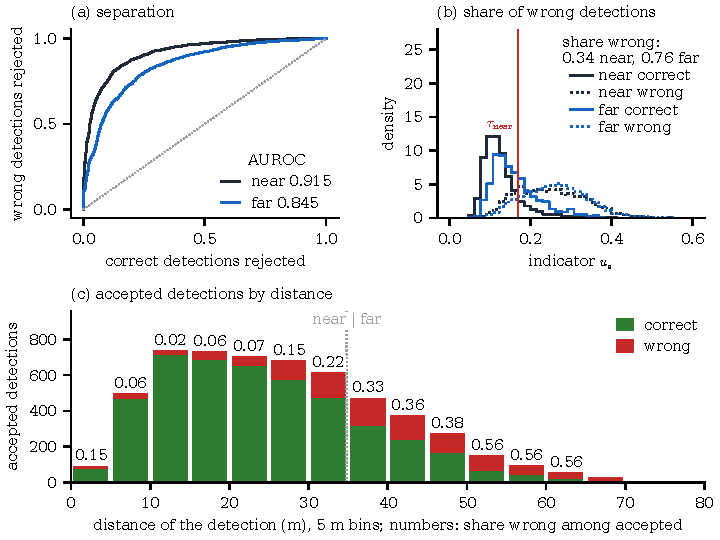
\includegraphics[width=\textwidth]{figures/fig_causes_kitti.pdf}
\caption{KITTI distance, spatial indicator, KITTI rule, split 0, threshold selected at near distance at the exploratory limit 0.1: (a) separation per distance condition, (b) indicator distributions, (c) accepted detections per 5\,m bin with the share of wrong ones among them (counts in the table above).}\label{fig:causes}
\end{figure}

\section{Division by recorded sequence}\label{sec:m7}
Frames of one recorded sequence share objects, weather and road, so they are not independent draws. The analysis was therefore repeated with the grid, selection and test parts drawn by recorded sequence: nuScenes scenes (m7, 150 scenes in the validation set) and KITTI drives (m8, 45 drives in the validation frames). The sequences are permuted by the split function of the division by frame, with the same seeds 0 to 4 and the same fractions, and every frame takes the part of its sequence. Limits, $\delta$, candidate thresholds and the boundary rule are unchanged. This analysis was added after the parameters had been fixed.

\paragraph{Variants.} \emph{Frame}: division by frame, as recorded. \emph{Variant (i)}: division by recorded sequence, the frame stays the unit of the selection test and of the HB bounds. \emph{Variant (ii)}: the same division with the sequence as the unit. The loss of sequence $s$ in condition $c$ is $\ell_s(\tau)=\frac{1}{|F_{s,c}|}\sum_{f\in F_{s,c}}a_f(\tau)$, where $F_{s,c}$ are the frames of $s$ that hold a car detection of $c$; a sequence without accepted detections has loss 0, and each sequence has equal weight. Retention is a sum over detections and is the same for both units. The post-hoc Method A (Section~\ref{sec:posthoc}) keeps the per-frame target exactly with the sequence as the unit.

\paragraph{Reproduction check.} Before the division by scene, the division by frame was rerun with the scripts of the scene runs and compared with the recorded results in every row and column: ``REPRODUCTION frame split: m3 1200 rows, m6 A/B/C all rows, input hashes: EQUAL'' (\path{results/m7_nuscenes_by_scene/REPRO_PASSED.txt}).

{\scriptsize
\begin{longtable}{lllllllp{3.6cm}}
\caption{nuScenes, division by recorded scene: outcome per split for the division by frame and variants (i) and (ii), and the retention of variant (ii) (--: no threshold). Cells without a selected threshold in any variant and split are not listed.}\label{tab:m7c}\\
\toprule
pair & ind. & $\alpha$ & cell & frame & (i) & (ii) & $R$ (ii), splits 0--4 \\
\midrule
\endfirsthead
\toprule
pair & ind. & $\alpha$ & cell & frame & (i) & (ii) & $R$ (ii), splits 0--4 \\
\midrule
\endhead
\bottomrule
\endfoot
distance & u\_e & $10^{-2}$ & far$\to$far & \texttt{?A?AA} & \texttt{AAAA?} & \texttt{-----} & -- -- -- -- -- \\
distance & u\_e & $10^{-2}$ & far$\to$near & \texttt{N??NN} & \texttt{????N} & \texttt{-----} & -- -- -- -- -- \\
distance & u\_e & $10^{-2}$ & near$\to$far & \texttt{AAAAA} & \texttt{AAAAA} & \texttt{-----} & -- -- -- -- -- \\
distance & u\_e & $10^{-2}$ & near$\to$near & \texttt{AAAA?} & \texttt{??AA?} & \texttt{-----} & -- -- -- -- -- \\
distance & u\_e & 0.05 & far$\to$far & \texttt{?A?AA} & \texttt{?AAA?} & \texttt{?????} & 0.01 0.02 0.02 0.03 0.02 \\
distance & u\_e & 0.05 & far$\to$near & \texttt{?????} & \texttt{???A?} & \texttt{?????} & 0.19 0.25 0.23 0.21 0.22 \\
distance & u\_e & 0.05 & near$\to$far & \texttt{AAAAA} & \texttt{AAA?N} & \texttt{??-??} & 0.00 0.00 -- 0.00 0.01 \\
distance & u\_e & 0.05 & near$\to$near & \texttt{?A??A} & \texttt{??A?N} & \texttt{??-??} & 0.03 0.03 -- 0.01 0.11 \\
distance & u\_e & 0.1 & far$\to$far & \texttt{????A} & \texttt{A?AA?} & \texttt{???A?} & 0.12 0.12 0.12 0.10 0.10 \\
distance & u\_e & 0.1 & far$\to$near & \texttt{AAAAA} & \texttt{AAAAA} & \texttt{?????} & 0.57 0.55 0.56 0.49 0.51 \\
distance & u\_e & 0.1 & near$\to$far & \texttt{NNNNN} & \texttt{NNNNN} & \texttt{A?A??} & 0.06 0.09 0.04 0.14 0.10 \\
distance & u\_e & 0.1 & near$\to$near & \texttt{AAA?A} & \texttt{A?AA?} & \texttt{??A??} & 0.44 0.49 0.37 0.55 0.51 \\
distance & u\_s & $10^{-2}$ & far$\to$far & \texttt{AA?A?} & \texttt{A?AAA} & \texttt{-----} & -- -- -- -- -- \\
distance & u\_s & $10^{-2}$ & far$\to$near & \texttt{?????} & \texttt{??AA?} & \texttt{-----} & -- -- -- -- -- \\
distance & u\_s & $10^{-2}$ & near$\to$far & \texttt{AAAAA} & \texttt{AAAAA} & \texttt{-----} & -- -- -- -- -- \\
distance & u\_s & $10^{-2}$ & near$\to$near & \texttt{AAAA?} & \texttt{AAAA?} & \texttt{-----} & -- -- -- -- -- \\
distance & u\_s & 0.05 & far$\to$far & \texttt{?A??A} & \texttt{A?AA?} & \texttt{-----} & -- -- -- -- -- \\
distance & u\_s & 0.05 & far$\to$near & \texttt{?A?A?} & \texttt{A?AA?} & \texttt{-----} & -- -- -- -- -- \\
distance & u\_s & 0.05 & near$\to$far & \texttt{AA?AA} & \texttt{A?A?N} & \texttt{----?} & -- -- -- -- 0.00 \\
distance & u\_s & 0.05 & near$\to$near & \texttt{?AAA?} & \texttt{AAAAN} & \texttt{----?} & -- -- -- -- 0.02 \\
distance & u\_s & 0.1 & far$\to$far & \texttt{????A} & \texttt{??AAN} & \texttt{A?AA?} & 0.03 0.05 0.03 0.03 0.05 \\
distance & u\_s & 0.1 & far$\to$near & \texttt{AAAAA} & \texttt{AAAAA} & \texttt{???A?} & 0.16 0.24 0.19 0.14 0.24 \\
distance & u\_s & 0.1 & near$\to$far & \texttt{NNNNN} & \texttt{NN?NN} & \texttt{A?A??} & 0.04 0.04 0.02 0.05 0.06 \\
distance & u\_s & 0.1 & near$\to$near & \texttt{A??AA} & \texttt{A?AA?} & \texttt{??AA?} & 0.17 0.20 0.11 0.20 0.27 \\
weather & u\_e & $10^{-2}$ & clear$\to$clear & \texttt{AAA??} & \texttt{??AA?} & \texttt{-----} & -- -- -- -- -- \\
weather & u\_e & $10^{-2}$ & clear$\to$rain & \texttt{?????} & \texttt{A??A?} & \texttt{-----} & -- -- -- -- -- \\
weather & u\_e & $10^{-2}$ & rain$\to$clear & \texttt{AAAAA} & \texttt{AA-A?} & \texttt{-----} & -- -- -- -- -- \\
weather & u\_e & $10^{-2}$ & rain$\to$rain & \texttt{?AAA?} & \texttt{A?-A?} & \texttt{-----} & -- -- -- -- -- \\
weather & u\_e & 0.05 & clear$\to$clear & \texttt{?A?A?} & \texttt{?AA??} & \texttt{-----} & -- -- -- -- -- \\
weather & u\_e & 0.05 & clear$\to$rain & \texttt{N????} & \texttt{?N??N} & \texttt{-----} & -- -- -- -- -- \\
weather & u\_e & 0.05 & rain$\to$clear & \texttt{AAAAA} & \texttt{AAAAA} & \texttt{-----} & -- -- -- -- -- \\
weather & u\_e & 0.05 & rain$\to$rain & \texttt{AA??A} & \texttt{A?AA?} & \texttt{-----} & -- -- -- -- -- \\
weather & u\_e & 0.1 & clear$\to$clear & \texttt{?A??A} & \texttt{??AAN} & \texttt{??A??} & 0.24 0.18 0.16 0.20 0.25 \\
weather & u\_e & 0.1 & clear$\to$rain & \texttt{NNNN?} & \texttt{?NNNN} & \texttt{?????} & 0.26 0.15 0.18 0.22 0.29 \\
weather & u\_e & 0.1 & rain$\to$clear & \texttt{AAAAA} & \texttt{AAAAA} & \texttt{-----} & -- -- -- -- -- \\
weather & u\_e & 0.1 & rain$\to$rain & \texttt{?A??A} & \texttt{A?AA?} & \texttt{-----} & -- -- -- -- -- \\
weather & u\_s & $10^{-2}$ & clear$\to$clear & \texttt{A---?} & \texttt{??-A?} & \texttt{-----} & -- -- -- -- -- \\
weather & u\_s & $10^{-2}$ & clear$\to$rain & \texttt{?---?} & \texttt{A?-??} & \texttt{-----} & -- -- -- -- -- \\
weather & u\_s & 0.05 & clear$\to$clear & \texttt{?AAA?} & \texttt{AAAA?} & \texttt{-----} & -- -- -- -- -- \\
weather & u\_s & 0.05 & clear$\to$rain & \texttt{?????} & \texttt{????N} & \texttt{-----} & -- -- -- -- -- \\
weather & u\_s & 0.05 & rain$\to$clear & \texttt{AAAAA} & \texttt{AAAAA} & \texttt{-----} & -- -- -- -- -- \\
weather & u\_s & 0.05 & rain$\to$rain & \texttt{?AAAA} & \texttt{AAAA?} & \texttt{-----} & -- -- -- -- -- \\
weather & u\_s & 0.1 & clear$\to$clear & \texttt{?A??A} & \texttt{??AAN} & \texttt{??A??} & 0.07 0.04 0.02 0.04 0.07 \\
weather & u\_s & 0.1 & clear$\to$rain & \texttt{N????} & \texttt{?N??N} & \texttt{?????} & 0.08 0.06 0.03 0.06 0.11 \\
weather & u\_s & 0.1 & rain$\to$clear & \texttt{AAAAA} & \texttt{AAAAA} & \texttt{-----} & -- -- -- -- -- \\
weather & u\_s & 0.1 & rain$\to$rain & \texttt{AAAAA} & \texttt{A?AA?} & \texttt{-----} & -- -- -- -- -- \\
\end{longtable}
}

\begin{table}[H]\centering\scriptsize
\caption{nuScenes scenes per condition and part under the division by scene, per split; in brackets the frames with a car detection (\texttt{results/m7\_nuscenes\_by\_scene/m7\_scene\_split\_summary.txt}, l.~94--98). A scene counts for near or far if it holds a car detection of that condition; most scenes count for both.}
\begin{tabular}{lllllll}\toprule split & grid / sel. / test & boundary & near sel. / test & far sel. / test & clear sel. / test & rain sel. / test \\ \midrule
0 & 15\,/\,68\,/\,67 & 19.888 m & 67\,/\,67 & 68\,/\,67 & 52 (1948)\,/\,49 (1908) & 9 (337)\,/\,10 (399) \\
1 & 15\,/\,68\,/\,67 & 19.975 m & 67\,/\,67 & 68\,/\,67 & 48 (1768)\,/\,50 (1952) & 11 (421)\,/\,11 (410) \\
2 & 15\,/\,68\,/\,67 & 21.211 m & 68\,/\,66 & 68\,/\,67 & 49 (1890)\,/\,52 (1964) & 11 (394)\,/\,9 (357) \\
3 & 15\,/\,68\,/\,67 & 18.154 m & 67\,/\,67 & 68\,/\,67 & 52 (2028)\,/\,47 (1746) & 10 (375)\,/\,12 (458) \\
4 & 15\,/\,68\,/\,67 & 19.694 m & 68\,/\,67 & 68\,/\,67 & 51 (1957)\,/\,51 (1980) & 9 (343)\,/\,10 (372) \\
\bottomrule\end{tabular}\end{table}

\begin{figure}[H]\centering
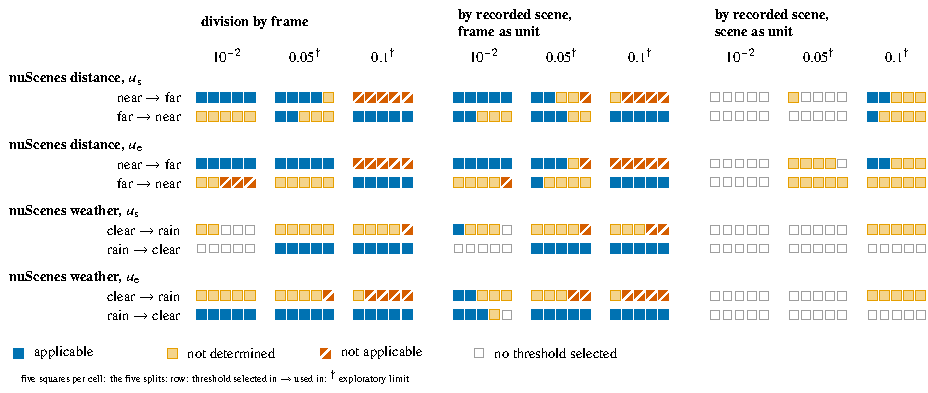
\includegraphics[width=\textwidth]{figures/fig_scenesplit.pdf}
\caption{nuScenes: outcomes per cell on the five splits for the division by frame, by recorded scene with the frame as unit, and by recorded scene with the scene as unit (drawn by \texttt{tools/figures/supplementary/supplementary\_figures.py} from \texttt{results/m7\_scene\_split/m7\_scene\_split.csv}).}\label{fig:scenesplit}
\end{figure}

\section{Division of KITTI by recorded drive}\label{sec:m8}
The KITTI object frames were mapped to their recorded drives with the mapping files of the KITTI object development kit; the 3{,}769 validation frames come from 45 drives. Before the division by drive, the division by frame was run again with the same code and compared with the recorded results: ``REPRODUCTION frame split: m6 A EQUAL, m6 B EQUAL, input hashes EQUAL''. Variant (i) keeps the frame as the unit of the selection test and of the interval; variant (ii) uses the drive, with the mean of the per-frame false acceptance proportions over the drive's frames in the condition as its loss. In the change of dataset and detector the nuScenes side is divided by recorded scene.

{\scriptsize
\begin{longtable}{p{3.0cm}p{0.9cm}p{0.6cm}lp{2.6cm}llll}
\caption{Outcome counts over the five splits, division by recorded drive (KITTI rule).}\label{tab:m8}\\
\toprule
setting & unit & ind. & $\alpha$ & transfer & A & N & ? & - \\
\midrule
\endfirsthead
\toprule
setting & unit & ind. & $\alpha$ & transfer & A & N & ? & - \\
\midrule
\endhead
\bottomrule
\endfoot
KITTI distance & drive & u\_e & $10^{-4}$ & far $\to$ near & 0 & 0 & 0 & 5 \\
KITTI distance & drive & u\_e & $10^{-4}$ & near $\to$ far & 0 & 0 & 0 & 5 \\
KITTI distance & drive & u\_e & $10^{-3}$ & far $\to$ near & 0 & 0 & 0 & 5 \\
KITTI distance & drive & u\_e & $10^{-3}$ & near $\to$ far & 0 & 0 & 0 & 5 \\
KITTI distance & drive & u\_e & $10^{-2}$ & far $\to$ near & 0 & 0 & 0 & 5 \\
KITTI distance & drive & u\_e & $10^{-2}$ & near $\to$ far & 0 & 0 & 0 & 5 \\
KITTI distance & drive & u\_e & 0.05 & far $\to$ near & 0 & 0 & 0 & 5 \\
KITTI distance & drive & u\_e & 0.05 & near $\to$ far & 0 & 0 & 0 & 5 \\
KITTI distance & drive & u\_e & 0.1 & far $\to$ near & 0 & 0 & 0 & 5 \\
KITTI distance & drive & u\_e & 0.1 & near $\to$ far & 0 & 0 & 0 & 5 \\
KITTI distance & drive & u\_s & $10^{-4}$ & far $\to$ near & 0 & 0 & 0 & 5 \\
KITTI distance & drive & u\_s & $10^{-4}$ & near $\to$ far & 0 & 0 & 0 & 5 \\
KITTI distance & drive & u\_s & $10^{-3}$ & far $\to$ near & 0 & 0 & 0 & 5 \\
KITTI distance & drive & u\_s & $10^{-3}$ & near $\to$ far & 0 & 0 & 0 & 5 \\
KITTI distance & drive & u\_s & $10^{-2}$ & far $\to$ near & 0 & 0 & 0 & 5 \\
KITTI distance & drive & u\_s & $10^{-2}$ & near $\to$ far & 0 & 0 & 0 & 5 \\
KITTI distance & drive & u\_s & 0.05 & far $\to$ near & 0 & 0 & 0 & 5 \\
KITTI distance & drive & u\_s & 0.05 & near $\to$ far & 0 & 0 & 0 & 5 \\
KITTI distance & drive & u\_s & 0.1 & far $\to$ near & 0 & 0 & 0 & 5 \\
KITTI distance & drive & u\_s & 0.1 & near $\to$ far & 0 & 0 & 0 & 5 \\
KITTI distance & frame & u\_e & $10^{-4}$ & far $\to$ near & 0 & 0 & 0 & 5 \\
KITTI distance & frame & u\_e & $10^{-4}$ & near $\to$ far & 0 & 0 & 0 & 5 \\
KITTI distance & frame & u\_e & $10^{-3}$ & far $\to$ near & 0 & 0 & 0 & 5 \\
KITTI distance & frame & u\_e & $10^{-3}$ & near $\to$ far & 0 & 0 & 0 & 5 \\
KITTI distance & frame & u\_e & $10^{-2}$ & far $\to$ near & 0 & 0 & 4 & 1 \\
KITTI distance & frame & u\_e & $10^{-2}$ & near $\to$ far & 2 & 0 & 2 & 1 \\
KITTI distance & frame & u\_e & 0.05 & far $\to$ near & 4 & 0 & 0 & 1 \\
KITTI distance & frame & u\_e & 0.05 & near $\to$ far & 0 & 3 & 2 & 0 \\
KITTI distance & frame & u\_e & 0.1 & far $\to$ near & 5 & 0 & 0 & 0 \\
KITTI distance & frame & u\_e & 0.1 & near $\to$ far & 0 & 5 & 0 & 0 \\
KITTI distance & frame & u\_s & $10^{-4}$ & far $\to$ near & 0 & 0 & 0 & 5 \\
KITTI distance & frame & u\_s & $10^{-4}$ & near $\to$ far & 0 & 0 & 0 & 5 \\
KITTI distance & frame & u\_s & $10^{-3}$ & far $\to$ near & 0 & 0 & 0 & 5 \\
KITTI distance & frame & u\_s & $10^{-3}$ & near $\to$ far & 0 & 0 & 0 & 5 \\
KITTI distance & frame & u\_s & $10^{-2}$ & far $\to$ near & 3 & 0 & 1 & 1 \\
KITTI distance & frame & u\_s & $10^{-2}$ & near $\to$ far & 1 & 1 & 2 & 1 \\
KITTI distance & frame & u\_s & 0.05 & far $\to$ near & 4 & 0 & 0 & 1 \\
KITTI distance & frame & u\_s & 0.05 & near $\to$ far & 0 & 5 & 0 & 0 \\
KITTI distance & frame & u\_s & 0.1 & far $\to$ near & 5 & 0 & 0 & 0 \\
KITTI distance & frame & u\_s & 0.1 & near $\to$ far & 0 & 5 & 0 & 0 \\
change of dataset & drive & u\_e & $10^{-4}$ & kitti $\to$ nuscenes & 0 & 0 & 0 & 5 \\
change of dataset & drive & u\_e & $10^{-4}$ & nuscenes $\to$ kitti & 0 & 0 & 0 & 5 \\
change of dataset & drive & u\_e & $10^{-3}$ & kitti $\to$ nuscenes & 0 & 0 & 0 & 5 \\
change of dataset & drive & u\_e & $10^{-3}$ & nuscenes $\to$ kitti & 0 & 0 & 0 & 5 \\
change of dataset & drive & u\_e & $10^{-2}$ & kitti $\to$ nuscenes & 0 & 0 & 0 & 5 \\
change of dataset & drive & u\_e & $10^{-2}$ & nuscenes $\to$ kitti & 0 & 0 & 0 & 5 \\
change of dataset & drive & u\_e & 0.05 & kitti $\to$ nuscenes & 0 & 0 & 0 & 5 \\
change of dataset & drive & u\_e & 0.05 & nuscenes $\to$ kitti & 0 & 0 & 5 & 0 \\
change of dataset & drive & u\_e & 0.1 & kitti $\to$ nuscenes & 0 & 0 & 0 & 5 \\
change of dataset & drive & u\_e & 0.1 & nuscenes $\to$ kitti & 0 & 0 & 5 & 0 \\
change of dataset & drive & u\_s & $10^{-4}$ & kitti $\to$ nuscenes & 0 & 0 & 0 & 5 \\
change of dataset & drive & u\_s & $10^{-4}$ & nuscenes $\to$ kitti & 0 & 0 & 0 & 5 \\
change of dataset & drive & u\_s & $10^{-3}$ & kitti $\to$ nuscenes & 0 & 0 & 0 & 5 \\
change of dataset & drive & u\_s & $10^{-3}$ & nuscenes $\to$ kitti & 0 & 0 & 0 & 5 \\
change of dataset & drive & u\_s & $10^{-2}$ & kitti $\to$ nuscenes & 0 & 0 & 0 & 5 \\
change of dataset & drive & u\_s & $10^{-2}$ & nuscenes $\to$ kitti & 0 & 0 & 0 & 5 \\
change of dataset & drive & u\_s & 0.05 & kitti $\to$ nuscenes & 0 & 0 & 0 & 5 \\
change of dataset & drive & u\_s & 0.05 & nuscenes $\to$ kitti & 0 & 0 & 5 & 0 \\
change of dataset & drive & u\_s & 0.1 & kitti $\to$ nuscenes & 0 & 0 & 0 & 5 \\
change of dataset & drive & u\_s & 0.1 & nuscenes $\to$ kitti & 0 & 0 & 5 & 0 \\
change of dataset & frame & u\_e & $10^{-4}$ & kitti $\to$ nuscenes & 0 & 0 & 0 & 5 \\
change of dataset & frame & u\_e & $10^{-4}$ & nuscenes $\to$ kitti & 0 & 0 & 0 & 5 \\
change of dataset & frame & u\_e & $10^{-3}$ & kitti $\to$ nuscenes & 0 & 0 & 0 & 5 \\
change of dataset & frame & u\_e & $10^{-3}$ & nuscenes $\to$ kitti & 0 & 0 & 0 & 5 \\
change of dataset & frame & u\_e & $10^{-2}$ & kitti $\to$ nuscenes & 2 & 0 & 3 & 0 \\
change of dataset & frame & u\_e & $10^{-2}$ & nuscenes $\to$ kitti & 4 & 0 & 1 & 0 \\
change of dataset & frame & u\_e & 0.05 & kitti $\to$ nuscenes & 2 & 2 & 1 & 0 \\
change of dataset & frame & u\_e & 0.05 & nuscenes $\to$ kitti & 5 & 0 & 0 & 0 \\
change of dataset & frame & u\_e & 0.1 & kitti $\to$ nuscenes & 2 & 1 & 2 & 0 \\
change of dataset & frame & u\_e & 0.1 & nuscenes $\to$ kitti & 4 & 0 & 1 & 0 \\
change of dataset & frame & u\_s & $10^{-4}$ & kitti $\to$ nuscenes & 0 & 0 & 0 & 5 \\
change of dataset & frame & u\_s & $10^{-4}$ & nuscenes $\to$ kitti & 0 & 0 & 0 & 5 \\
change of dataset & frame & u\_s & $10^{-3}$ & kitti $\to$ nuscenes & 0 & 0 & 0 & 5 \\
change of dataset & frame & u\_s & $10^{-3}$ & nuscenes $\to$ kitti & 0 & 0 & 0 & 5 \\
change of dataset & frame & u\_s & $10^{-2}$ & kitti $\to$ nuscenes & 5 & 0 & 0 & 0 \\
change of dataset & frame & u\_s & $10^{-2}$ & nuscenes $\to$ kitti & 0 & 5 & 0 & 0 \\
change of dataset & frame & u\_s & 0.05 & kitti $\to$ nuscenes & 5 & 0 & 0 & 0 \\
change of dataset & frame & u\_s & 0.05 & nuscenes $\to$ kitti & 0 & 5 & 0 & 0 \\
change of dataset & frame & u\_s & 0.1 & kitti $\to$ nuscenes & 5 & 0 & 0 & 0 \\
change of dataset & frame & u\_s & 0.1 & nuscenes $\to$ kitti & 0 & 5 & 0 & 0 \\
\end{longtable}
}

{\scriptsize
\begin{longtable}{p{4.6cm}llp{1.6cm}ll}
\caption{Drives and frames with a car detection per part and condition, division by recorded drive.}\label{tab:m8drv}\\
\toprule
setting & split & part & condition & drives & frames \\
\midrule
\endfirsthead
\toprule
setting & split & part & condition & drives & frames \\
\midrule
\endhead
\bottomrule
\endfoot
KITTI distance & 0 & grid & near & 4 & 543 \\
KITTI distance & 0 & grid & far & 3 & 537 \\
KITTI distance & 0 & select & near & 19 & 714 \\
KITTI distance & 0 & select & far & 11 & 645 \\
KITTI distance & 0 & eval & near & 21 & 2065 \\
KITTI distance & 0 & eval & far & 12 & 2200 \\
change of dataset (KITTI side) & 0 & select & KITTI & 22 & 1144 \\
change of dataset (KITTI side) & 0 & eval & KITTI & 23 & 2552 \\
KITTI distance & 1 & grid & near & 4 & 295 \\
KITTI distance & 1 & grid & far & 3 & 291 \\
KITTI distance & 1 & select & near & 19 & 1057 \\
KITTI distance & 1 & select & far & 11 & 1009 \\
KITTI distance & 1 & eval & near & 21 & 1949 \\
KITTI distance & 1 & eval & far & 12 & 2097 \\
change of dataset (KITTI side) & 1 & select & KITTI & 22 & 1155 \\
change of dataset (KITTI side) & 1 & eval & KITTI & 23 & 2541 \\
KITTI distance & 2 & grid & near & 2 & 260 \\
KITTI distance & 2 & grid & far & 4 & 272 \\
KITTI distance & 2 & select & near & 16 & 1737 \\
KITTI distance & 2 & select & far & 20 & 2336 \\
KITTI distance & 2 & eval & near & 17 & 826 \\
KITTI distance & 2 & eval & far & 20 & 987 \\
change of dataset (KITTI side) & 2 & select & KITTI & 22 & 2323 \\
change of dataset (KITTI side) & 2 & eval & KITTI & 23 & 1373 \\
KITTI distance & 3 & grid & near & 4 & 297 \\
KITTI distance & 3 & grid & far & 2 & 317 \\
KITTI distance & 3 & select & near & 19 & 1091 \\
KITTI distance & 3 & select & far & 12 & 1021 \\
KITTI distance & 3 & eval & near & 20 & 1859 \\
KITTI distance & 3 & eval & far & 12 & 2086 \\
change of dataset (KITTI side) & 3 & select & KITTI & 22 & 1456 \\
change of dataset (KITTI side) & 3 & eval & KITTI & 23 & 2240 \\
KITTI distance & 4 & grid & near & 4 & 34 \\
KITTI distance & 4 & grid & far & 2 & 31 \\
KITTI distance & 4 & select & near & 20 & 1303 \\
KITTI distance & 4 & select & far & 11 & 1232 \\
KITTI distance & 4 & eval & near & 20 & 1973 \\
KITTI distance & 4 & eval & far & 13 & 2128 \\
change of dataset (KITTI side) & 4 & select & KITTI & 22 & 1412 \\
change of dataset (KITTI side) & 4 & eval & KITTI & 23 & 2284 \\
\end{longtable}
}

\begin{figure}[H]\centering
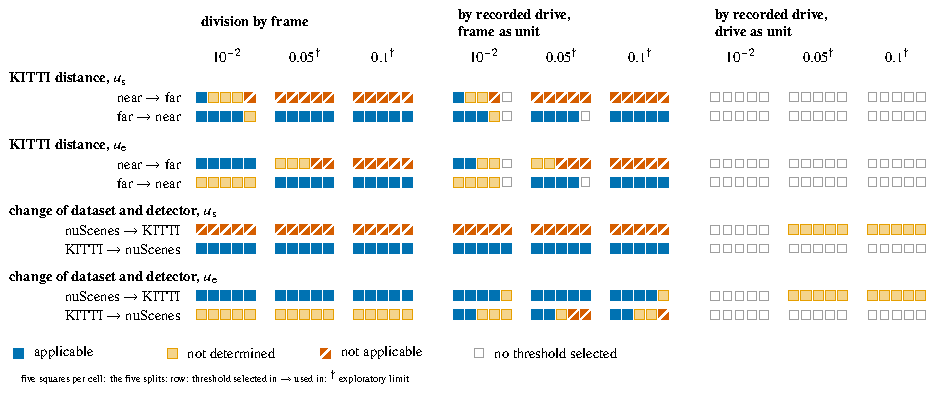
\includegraphics[width=\textwidth]{figures/fig_drivesplit.pdf}
\caption{KITTI with the KITTI rule: outcomes per cell on the five splits for the division by frame, by recorded drive with the frame as unit, and by recorded drive with the drive as unit. In the change of dataset and detector the nuScenes side is divided by recorded scene.}\label{fig:drivesplit}
\end{figure}

\section{Retention, shares of wrong detections, intervals, frames and the common threshold (division by frame)}\label{sec:review}

{\scriptsize
\begin{longtable}{p{2.4cm}p{2.4cm}p{0.6cm}p{2.2cm}llll}
\caption{Every applicable transfer at $10^{-2}$ with its retention $R$ (share of correct detections kept).}\label{tab:A1}\\
\toprule
setting & division & ind. & transfer & split & $A$ & $[L,U]$ & $R$ \\
\midrule
\endfirsthead
\toprule
setting & division & ind. & transfer & split & $A$ & $[L,U]$ & $R$ \\
\midrule
\endhead
\bottomrule
\endfoot
KITTI distance & frame & u\_e & near $\to$ far & 0 & 0.0013 & [0.0001, 0.0055] & 0.0489 \\
KITTI distance & frame & u\_e & near $\to$ far & 1 & 0.0013 & [0.0001, 0.0055] & 0.0692 \\
KITTI distance & frame & u\_e & near $\to$ far & 2 & 0.0013 & [0.0001, 0.0056] & 0.0355 \\
KITTI distance & frame & u\_e & near $\to$ far & 3 & 0.0032 & [0.0008, 0.0085] & 0.1113 \\
KITTI distance & frame & u\_e & near $\to$ far & 4 & 0.0000 & [0.0000, 0.0024] & 0.0570 \\
KITTI distance & frame & u\_s & far $\to$ near & 0 & 0.0040 & [0.0012, 0.0098] & 0.1498 \\
KITTI distance & frame & u\_s & far $\to$ near & 1 & 0.0007 & [0.0000, 0.0045] & 0.0546 \\
KITTI distance & frame & u\_s & far $\to$ near & 3 & 0.0000 & [0.0000, 0.0025] & 0.0417 \\
KITTI distance & frame & u\_s & far $\to$ near & 4 & 0.0020 & [0.0003, 0.0069] & 0.1048 \\
KITTI distance & frame & u\_s & near $\to$ far & 1 & 0.0019 & [0.0003, 0.0066] & 0.0185 \\
change of dataset & frame & u\_e & nuScenes $\to$ KITTI & 0 & 0.0023 & [0.0004, 0.0067] & 0.2347 \\
change of dataset & frame & u\_e & nuScenes $\to$ KITTI & 1 & 0.0024 & [0.0005, 0.0070] & 0.2361 \\
change of dataset & frame & u\_e & nuScenes $\to$ KITTI & 2 & 0.0011 & [0.0001, 0.0046] & 0.2316 \\
change of dataset & frame & u\_e & nuScenes $\to$ KITTI & 3 & 0.0024 & [0.0005, 0.0070] & 0.2402 \\
change of dataset & frame & u\_e & nuScenes $\to$ KITTI & 4 & 0.0036 & [0.0010, 0.0087] & 0.2851 \\
change of dataset & frame & u\_s & KITTI $\to$ nuScenes & 0 & 0.0000 & [0.0000, 0.0013] & 0.0002 \\
change of dataset & frame & u\_s & KITTI $\to$ nuScenes & 1 & 0.0000 & [0.0000, 0.0013] & 0.0000 \\
change of dataset & frame & u\_s & KITTI $\to$ nuScenes & 2 & 0.0000 & [0.0000, 0.0013] & 0.0002 \\
change of dataset & frame & u\_s & KITTI $\to$ nuScenes & 3 & 0.0000 & [0.0000, 0.0013] & 0.0000 \\
change of dataset & frame & u\_s & KITTI $\to$ nuScenes & 4 & 0.0000 & [0.0000, 0.0013] & 0.0001 \\
nuScenes distance & frame & u\_e & near $\to$ far & 0 & 0.0000 & [0.0000, 0.0016] & 0.0034 \\
nuScenes distance & frame & u\_e & near $\to$ far & 1 & 0.0000 & [0.0000, 0.0016] & 0.0021 \\
nuScenes distance & frame & u\_e & near $\to$ far & 2 & 0.0000 & [0.0000, 0.0016] & 0.0038 \\
nuScenes distance & frame & u\_e & near $\to$ far & 3 & 0.0000 & [0.0000, 0.0016] & 0.0047 \\
nuScenes distance & frame & u\_e & near $\to$ far & 4 & 0.0002 & [0.0000, 0.0024] & 0.0107 \\
nuScenes distance & frame & u\_s & near $\to$ far & 0 & 0.0024 & [0.0006, 0.0064] & 0.0046 \\
nuScenes distance & frame & u\_s & near $\to$ far & 1 & 0.0007 & [0.0000, 0.0034] & 0.0030 \\
nuScenes distance & frame & u\_s & near $\to$ far & 2 & 0.0022 & [0.0005, 0.0058] & 0.0042 \\
nuScenes distance & frame & u\_s & near $\to$ far & 3 & 0.0033 & [0.0010, 0.0076] & 0.0047 \\
nuScenes distance & frame & u\_s & near $\to$ far & 4 & 0.0040 & [0.0015, 0.0083] & 0.0059 \\
nuScenes distance & scene (i) frame unit & u\_e & near $\to$ far & 0 & 0.0000 & [0.0000, 0.0015] & 0.0044 \\
nuScenes distance & scene (i) frame unit & u\_e & near $\to$ far & 1 & 0.0000 & [0.0000, 0.0015] & 0.0090 \\
nuScenes distance & scene (i) frame unit & u\_e & near $\to$ far & 2 & 0.0000 & [0.0000, 0.0016] & 0.0040 \\
nuScenes distance & scene (i) frame unit & u\_e & near $\to$ far & 3 & 0.0000 & [0.0000, 0.0016] & 0.0024 \\
nuScenes distance & scene (i) frame unit & u\_e & near $\to$ far & 4 & 0.0023 & [0.0006, 0.0062] & 0.0150 \\
nuScenes distance & scene (i) frame unit & u\_s & far $\to$ near & 2 & 0.0030 & [0.0008, 0.0074] & 0.0252 \\
nuScenes distance & scene (i) frame unit & u\_s & far $\to$ near & 3 & 0.0031 & [0.0009, 0.0075] & 0.0312 \\
nuScenes distance & scene (i) frame unit & u\_s & near $\to$ far & 0 & 0.0019 & [0.0004, 0.0054] & 0.0055 \\
nuScenes distance & scene (i) frame unit & u\_s & near $\to$ far & 1 & 0.0038 & [0.0014, 0.0079] & 0.0037 \\
nuScenes distance & scene (i) frame unit & u\_s & near $\to$ far & 2 & 0.0011 & [0.0001, 0.0042] & 0.0038 \\
nuScenes distance & scene (i) frame unit & u\_s & near $\to$ far & 3 & 0.0042 & [0.0017, 0.0086] & 0.0069 \\
nuScenes distance & scene (i) frame unit & u\_s & near $\to$ far & 4 & 0.0045 & [0.0017, 0.0092] & 0.0075 \\
nuScenes rain & frame & u\_e & rain $\to$ clear & 0 & 0.0016 & [0.0002, 0.0053] & 0.0257 \\
nuScenes rain & frame & u\_e & rain $\to$ clear & 1 & 0.0000 & [0.0000, 0.0019] & 0.0116 \\
nuScenes rain & frame & u\_e & rain $\to$ clear & 2 & 0.0000 & [0.0000, 0.0019] & 0.0166 \\
nuScenes rain & frame & u\_e & rain $\to$ clear & 3 & 0.0016 & [0.0002, 0.0053] & 0.0299 \\
nuScenes rain & frame & u\_e & rain $\to$ clear & 4 & 0.0038 & [0.0012, 0.0090] & 0.0578 \\
nuScenes rain & scene (i) frame unit & u\_e & clear $\to$ rain & 0 & 0.0000 & [0.0000, 0.0092] & 0.1009 \\
nuScenes rain & scene (i) frame unit & u\_e & clear $\to$ rain & 3 & 0.0000 & [0.0000, 0.0080] & 0.0393 \\
nuScenes rain & scene (i) frame unit & u\_e & rain $\to$ clear & 0 & 0.0005 & [0.0000, 0.0034] & 0.0210 \\
nuScenes rain & scene (i) frame unit & u\_e & rain $\to$ clear & 1 & 0.0029 & [0.0007, 0.0075] & 0.0575 \\
nuScenes rain & scene (i) frame unit & u\_e & rain $\to$ clear & 3 & 0.0000 & [0.0000, 0.0021] & 0.0048 \\
nuScenes rain & scene (i) frame unit & u\_s & clear $\to$ rain & 0 & 0.0000 & [0.0000, 0.0092] & 0.0214 \\
\end{longtable}
}

{\scriptsize
\begin{longtable}{p{3.0cm}p{2.2cm}p{0.5cm}llllll}
\caption{Car detections, share of wrong ones and median indicator value per condition, split 0 (all parts, and the test part).}\label{tab:A2}\\
\toprule
setting & condition & ind. & part & det. & wrong & med. & med. corr. & med. wrong \\
\midrule
\endfirsthead
\toprule
setting & condition & ind. & part & det. & wrong & med. & med. corr. & med. wrong \\
\midrule
\endhead
\bottomrule
\endfoot
KITTI distance (KITTI rule) & near & u\_s & all & 14031 & 0.342 & 0.141 & 0.118 & 0.244 \\
KITTI distance (KITTI rule) & near & u\_e & all & 14031 & 0.342 & 0.216 & 0.132 & 0.748 \\
KITTI distance (KITTI rule) & far & u\_s & all & 13144 & 0.763 & 0.235 & 0.150 & 0.259 \\
KITTI distance (KITTI rule) & far & u\_e & all & 13144 & 0.763 & 0.779 & 0.327 & 0.823 \\
nuScenes distance & near & u\_s & all & 20227 & 0.187 & 0.214 & 0.206 & 0.266 \\
nuScenes distance & near & u\_e & all & 20227 & 0.187 & 0.274 & 0.242 & 0.621 \\
nuScenes distance & far & u\_s & all & 19809 & 0.514 & 0.306 & 0.285 & 0.326 \\
nuScenes distance & far & u\_e & all & 19809 & 0.514 & 0.604 & 0.480 & 0.738 \\
nuScenes rain & clear & u\_s & all & 30727 & 0.335 & 0.254 & 0.230 & 0.310 \\
nuScenes rain & clear & u\_e & all & 30727 & 0.335 & 0.436 & 0.331 & 0.719 \\
nuScenes rain & rain & u\_s & all & 6858 & 0.416 & 0.263 & 0.231 & 0.311 \\
nuScenes rain & rain & u\_e & all & 6858 & 0.416 & 0.451 & 0.301 & 0.702 \\
KITTI distance (KITTI rule) & near & u\_s & eval & 6310 & 0.336 & 0.139 & 0.117 & 0.246 \\
KITTI distance (KITTI rule) & near & u\_e & eval & 6310 & 0.336 & 0.212 & 0.131 & 0.742 \\
KITTI distance (KITTI rule) & far & u\_s & eval & 5957 & 0.763 & 0.235 & 0.151 & 0.259 \\
KITTI distance (KITTI rule) & far & u\_e & eval & 5957 & 0.763 & 0.777 & 0.329 & 0.823 \\
nuScenes distance & near & u\_s & eval & 9099 & 0.189 & 0.215 & 0.206 & 0.266 \\
nuScenes distance & near & u\_e & eval & 9099 & 0.189 & 0.275 & 0.244 & 0.614 \\
nuScenes distance & far & u\_s & eval & 8990 & 0.516 & 0.305 & 0.283 & 0.328 \\
nuScenes distance & far & u\_e & eval & 8990 & 0.516 & 0.601 & 0.482 & 0.734 \\
nuScenes rain & clear & u\_s & eval & 13857 & 0.336 & 0.254 & 0.229 & 0.311 \\
nuScenes rain & clear & u\_e & eval & 13857 & 0.336 & 0.436 & 0.332 & 0.714 \\
nuScenes rain & rain & u\_s & eval & 3122 & 0.425 & 0.264 & 0.232 & 0.310 \\
nuScenes rain & rain & u\_e & eval & 3122 & 0.425 & 0.465 & 0.313 & 0.700 \\
change of dataset & KITTI (KITTI rule) & u\_s & all & 27175 & 0.546 & 0.184 & 0.125 & 0.254 \\
change of dataset & KITTI (KITTI rule) & u\_e & all & 27175 & 0.546 & 0.545 & 0.168 & 0.804 \\
change of dataset & KITTI (as run) & u\_s & all & 29629 & 0.583 & 0.187 & 0.125 & 0.250 \\
change of dataset & KITTI (as run) & u\_e & all & 29629 & 0.583 & 0.573 & 0.168 & 0.794 \\
change of dataset & nuScenes & u\_s & all & 40036 & 0.349 & 0.256 & 0.229 & 0.311 \\
change of dataset & nuScenes & u\_e & all & 40036 & 0.349 & 0.439 & 0.325 & 0.720 \\
change of dataset & KITTI (KITTI rule) & u\_s & eval & 13707 & 0.544 & 0.184 & 0.124 & 0.255 \\
change of dataset & KITTI (KITTI rule) & u\_e & eval & 13707 & 0.544 & 0.543 & 0.168 & 0.803 \\
change of dataset & KITTI (as run) & u\_s & eval & 14940 & 0.581 & 0.187 & 0.124 & 0.250 \\
change of dataset & KITTI (as run) & u\_e & eval & 14940 & 0.581 & 0.570 & 0.168 & 0.793 \\
change of dataset & nuScenes & u\_s & eval & 19999 & 0.350 & 0.255 & 0.229 & 0.311 \\
change of dataset & nuScenes & u\_e & eval & 19999 & 0.350 & 0.443 & 0.329 & 0.714 \\
\end{longtable}
}

{\scriptsize
\begin{longtable}{p{3.0cm}p{0.6cm}lllllp{0.6cm}}
\caption{Every clear $\to$ rain cell with a selected threshold (frame = division by frame; scene (i)/(ii) = division by recorded scene with the frame / scene as unit).}\label{tab:A3}\\
\toprule
division & ind. & $\alpha$ & split & $A$ & $[L,U]$ & $R$ & out. \\
\midrule
\endfirsthead
\toprule
division & ind. & $\alpha$ & split & $A$ & $[L,U]$ & $R$ & out. \\
\midrule
\endhead
\bottomrule
\endfoot
frame & u\_e & $10^{-2}$ & 0 & 0.0024 & [0.0000, 0.0158] & 0.087 & ? \\
frame & u\_e & $10^{-2}$ & 1 & 0.0025 & [0.0000, 0.0162] & 0.091 & ? \\
frame & u\_e & $10^{-2}$ & 2 & 0.0037 & [0.0001, 0.0188] & 0.102 & ? \\
frame & u\_e & $10^{-2}$ & 3 & 0.0050 & [0.0004, 0.0209] & 0.102 & ? \\
frame & u\_e & $10^{-2}$ & 4 & 0.0101 & [0.0020, 0.0292] & 0.126 & ? \\
frame & u\_e & 0.05 & 0 & 0.0871 & [0.0573, 0.1278] & 0.421 & N \\
frame & u\_e & 0.05 & 1 & 0.0608 & [0.0351, 0.0963] & 0.402 & ? \\
frame & u\_e & 0.05 & 2 & 0.0694 & [0.0409, 0.1052] & 0.433 & ? \\
frame & u\_e & 0.05 & 3 & 0.0665 & [0.0389, 0.1020] & 0.417 & ? \\
frame & u\_e & 0.05 & 4 & 0.0650 & [0.0375, 0.1005] & 0.439 & ? \\
frame & u\_e & 0.1 & 0 & 0.1699 & [0.1279, 0.2196] & 0.722 & N \\
frame & u\_e & 0.1 & 1 & 0.1449 & [0.1052, 0.1927] & 0.723 & N \\
frame & u\_e & 0.1 & 2 & 0.1527 & [0.1117, 0.2009] & 0.747 & N \\
frame & u\_e & 0.1 & 3 & 0.1571 & [0.1158, 0.2059] & 0.714 & N \\
frame & u\_e & 0.1 & 4 & 0.1350 & [0.0957, 0.1812] & 0.729 & ? \\
frame & u\_s & $10^{-2}$ & 0 & 0.0048 & [0.0003, 0.0204] & 0.026 & ? \\
frame & u\_s & $10^{-2}$ & 4 & 0.0197 & [0.0062, 0.0436] & 0.038 & ? \\
frame & u\_s & 0.05 & 0 & 0.0673 & [0.0398, 0.1024] & 0.162 & ? \\
frame & u\_s & 0.05 & 1 & 0.0518 & [0.0275, 0.0843] & 0.144 & ? \\
frame & u\_s & 0.05 & 2 & 0.0589 & [0.0332, 0.0933] & 0.159 & ? \\
frame & u\_s & 0.05 & 3 & 0.0512 & [0.0275, 0.0841] & 0.170 & ? \\
frame & u\_s & 0.05 & 4 & 0.0628 & [0.0375, 0.0975] & 0.202 & ? \\
frame & u\_s & 0.1 & 0 & 0.1401 & [0.1003, 0.1851] & 0.385 & N \\
frame & u\_s & 0.1 & 1 & 0.1372 & [0.0988, 0.1845] & 0.382 & ? \\
frame & u\_s & 0.1 & 2 & 0.1353 & [0.0966, 0.1817] & 0.399 & ? \\
frame & u\_s & 0.1 & 3 & 0.1214 & [0.0857, 0.1675] & 0.421 & ? \\
frame & u\_s & 0.1 & 4 & 0.1219 & [0.0849, 0.1671] & 0.394 & ? \\
scene (i) frame unit & u\_e & $10^{-2}$ & 0 & 0.0000 & [0.0000, 0.0092] & 0.101 & A \\
scene (i) frame unit & u\_e & $10^{-2}$ & 1 & 0.0085 & [0.0013, 0.0273] & 0.092 & ? \\
scene (i) frame unit & u\_e & $10^{-2}$ & 2 & 0.0042 & [0.0001, 0.0212] & 0.084 & ? \\
scene (i) frame unit & u\_e & $10^{-2}$ & 3 & 0.0000 & [0.0000, 0.0080] & 0.039 & A \\
scene (i) frame unit & u\_e & $10^{-2}$ & 4 & 0.0101 & [0.0016, 0.0311] & 0.142 & ? \\
scene (i) frame unit & u\_e & 0.05 & 0 & 0.0602 & [0.0354, 0.0972] & 0.453 & ? \\
scene (i) frame unit & u\_e & 0.05 & 1 & 0.0929 & [0.0619, 0.1346] & 0.339 & N \\
scene (i) frame unit & u\_e & 0.05 & 2 & 0.0692 & [0.0397, 0.1084] & 0.422 & ? \\
scene (i) frame unit & u\_e & 0.05 & 3 & 0.0708 & [0.0446, 0.1056] & 0.406 & ? \\
scene (i) frame unit & u\_e & 0.05 & 4 & 0.1015 & [0.0661, 0.1450] & 0.398 & N \\
scene (i) frame unit & u\_e & 0.1 & 0 & 0.1386 & [0.0998, 0.1863] & 0.720 & ? \\
scene (i) frame unit & u\_e & 0.1 & 1 & 0.2098 & [0.1642, 0.2638] & 0.701 & N \\
scene (i) frame unit & u\_e & 0.1 & 2 & 0.1442 & [0.1021, 0.1951] & 0.726 & N \\
scene (i) frame unit & u\_e & 0.1 & 3 & 0.1431 & [0.1057, 0.1871] & 0.665 & N \\
scene (i) frame unit & u\_e & 0.1 & 4 & 0.2360 & [0.1840, 0.2926] & 0.775 & N \\
scene (i) frame unit & u\_s & $10^{-2}$ & 0 & 0.0000 & [0.0000, 0.0092] & 0.021 & A \\
scene (i) frame unit & u\_s & $10^{-2}$ & 1 & 0.0061 & [0.0006, 0.0231] & 0.025 & ? \\
scene (i) frame unit & u\_s & $10^{-2}$ & 3 & 0.0066 & [0.0009, 0.0220] & 0.014 & ? \\
scene (i) frame unit & u\_s & $10^{-2}$ & 4 & 0.0121 & [0.0024, 0.0344] & 0.039 & ? \\
scene (i) frame unit & u\_s & 0.05 & 0 & 0.0288 & [0.0119, 0.0568] & 0.150 & ? \\
scene (i) frame unit & u\_s & 0.05 & 1 & 0.0720 & [0.0441, 0.1091] & 0.169 & ? \\
scene (i) frame unit & u\_s & 0.05 & 2 & 0.0449 & [0.0229, 0.0811] & 0.183 & ? \\
scene (i) frame unit & u\_s & 0.05 & 3 & 0.0537 & [0.0308, 0.0849] & 0.129 & ? \\
scene (i) frame unit & u\_s & 0.05 & 4 & 0.1067 & [0.0706, 0.1511] & 0.230 & N \\
scene (i) frame unit & u\_s & 0.1 & 0 & 0.0989 & [0.0657, 0.1411] & 0.374 & ? \\
scene (i) frame unit & u\_s & 0.1 & 1 & 0.1490 & [0.1098, 0.1976] & 0.384 & N \\
scene (i) frame unit & u\_s & 0.1 & 2 & 0.1098 & [0.0736, 0.1573] & 0.374 & ? \\
scene (i) frame unit & u\_s & 0.1 & 3 & 0.1252 & [0.0905, 0.1677] & 0.336 & ? \\
scene (i) frame unit & u\_s & 0.1 & 4 & 0.2189 & [0.1693, 0.2754] & 0.439 & N \\
scene (ii) scene unit & u\_e & 0.1 & 0 & 0.0181 & [0.0000, 0.3619] & 0.260 & ? \\
scene (ii) scene unit & u\_e & 0.1 & 1 & 0.0242 & [0.0000, 0.3525] & 0.155 & ? \\
scene (ii) scene unit & u\_e & 0.1 & 2 & 0.0037 & [0.0000, 0.3508] & 0.176 & ? \\
scene (ii) scene unit & u\_e & 0.1 & 3 & 0.0285 & [0.0000, 0.3417] & 0.216 & ? \\
scene (ii) scene unit & u\_e & 0.1 & 4 & 0.0491 & [0.0000, 0.4228] & 0.286 & ? \\
scene (ii) scene unit & u\_s & 0.1 & 0 & 0.0106 & [0.0000, 0.3434] & 0.078 & ? \\
scene (ii) scene unit & u\_s & 0.1 & 1 & 0.0220 & [0.0000, 0.3477] & 0.059 & ? \\
scene (ii) scene unit & u\_s & 0.1 & 2 & 0.0069 & [0.0000, 0.3607] & 0.026 & ? \\
scene (ii) scene unit & u\_s & 0.1 & 3 & 0.0222 & [0.0000, 0.3283] & 0.058 & ? \\
scene (ii) scene unit & u\_s & 0.1 & 4 & 0.0563 & [0.0000, 0.4350] & 0.113 & ? \\
\end{longtable}
}

{\scriptsize
\begin{longtable}{p{4.6cm}p{3.2cm}lll}
\caption{Frames per condition in the selection and test parts (division by frame).}\label{tab:A4}\\
\toprule
setting & condition & split & selection frames & test frames \\
\midrule
\endfirsthead
\toprule
setting & condition & split & selection frames & test frames \\
\midrule
\endhead
\bottomrule
\endfoot
KITTI distance (KITTI rule) & near & 0 & 1484 & 1500 \\
KITTI distance (KITTI rule) & far & 0 & 1514 & 1545 \\
nuScenes distance & near & 0 & 2207 & 2209 \\
nuScenes distance & far & 0 & 2270 & 2276 \\
nuScenes rain & clear & 0 & 1917 & 1900 \\
nuScenes rain & rain & 0 & 392 & 414 \\
change of dataset & KITTI (KITTI rule) & 0 & 1844 & 1852 \\
change of dataset & nuScenes & 0 & 2849 & 2850 \\
KITTI distance (KITTI rule) & near & 1 & 1467 & 1461 \\
KITTI distance (KITTI rule) & far & 1 & 1540 & 1539 \\
nuScenes distance & near & 1 & 2214 & 2198 \\
nuScenes distance & far & 1 & 2289 & 2270 \\
nuScenes rain & clear & 1 & 1900 & 1915 \\
nuScenes rain & rain & 1 & 417 & 403 \\
change of dataset & KITTI (KITTI rule) & 1 & 1844 & 1852 \\
change of dataset & nuScenes & 1 & 2859 & 2840 \\
KITTI distance (KITTI rule) & near & 2 & 1482 & 1495 \\
KITTI distance (KITTI rule) & far & 2 & 1523 & 1527 \\
nuScenes distance & near & 2 & 2195 & 2175 \\
nuScenes distance & far & 2 & 2311 & 2289 \\
nuScenes rain & clear & 2 & 1900 & 1898 \\
nuScenes rain & rain & 2 & 422 & 403 \\
change of dataset & KITTI (KITTI rule) & 2 & 1848 & 1848 \\
change of dataset & nuScenes & 2 & 2863 & 2836 \\
KITTI distance (KITTI rule) & near & 3 & 1466 & 1473 \\
KITTI distance (KITTI rule) & far & 3 & 1525 & 1551 \\
nuScenes distance & near & 3 & 2183 & 2172 \\
nuScenes distance & far & 3 & 2310 & 2304 \\
nuScenes rain & clear & 3 & 1917 & 1902 \\
nuScenes rain & rain & 3 & 409 & 404 \\
change of dataset & KITTI (KITTI rule) & 3 & 1844 & 1852 \\
change of dataset & nuScenes & 3 & 2847 & 2852 \\
KITTI distance (KITTI rule) & near & 4 & 1471 & 1474 \\
KITTI distance (KITTI rule) & far & 4 & 1560 & 1536 \\
nuScenes distance & near & 4 & 2199 & 2205 \\
nuScenes distance & far & 4 & 2300 & 2265 \\
nuScenes rain & clear & 4 & 1932 & 1896 \\
nuScenes rain & rain & 4 & 399 & 398 \\
change of dataset & KITTI (KITTI rule) & 4 & 1847 & 1849 \\
change of dataset & nuScenes & 4 & 2861 & 2838 \\
\end{longtable}
}

{\scriptsize
\begin{longtable}{p{2.9cm}p{0.6cm}llllllllll}
\caption{The common threshold $\tau^*$ on the test part of each distance condition, with the retention gap $G=R(\tau_c)-R(\tau^*)$.}\label{tab:A5}\\
\toprule
setting & ind. & $\alpha$ & condition & split & $\tau^*$ & $A$ & $[L,U]$ & out. & $R(\tau^*)$ & $G$ \\
\midrule
\endfirsthead
\toprule
setting & ind. & $\alpha$ & condition & split & $\tau^*$ & $A$ & $[L,U]$ & out. & $R(\tau^*)$ & $G$ \\
\midrule
\endhead
\bottomrule
\endfoot
KITTI distance (KITTI rule) & u\_s & $10^{-2}$ & near & 0 & 0.0890 & 0.0040 & [0.0012, 0.0098] & A & 0.150 & 0.050 \\
KITTI distance (KITTI rule) & u\_s & $10^{-2}$ & far & 0 & 0.0890 & 0.0078 & [0.0035, 0.0148] & ? & 0.030 & 0.000 \\
KITTI distance (KITTI rule) & u\_s & 0.05 & near & 0 & 0.1098 & 0.0126 & [0.0064, 0.0213] & A & 0.408 & 0.311 \\
KITTI distance (KITTI rule) & u\_s & 0.05 & far & 0 & 0.1098 & 0.0324 & [0.0227, 0.0446] & A & 0.140 & 0.024 \\
KITTI distance (KITTI rule) & u\_s & 0.1 & near & 0 & 0.1270 & 0.0233 & [0.0151, 0.0350] & A & 0.604 & 0.262 \\
KITTI distance (KITTI rule) & u\_s & 0.1 & far & 0 & 0.1270 & 0.0702 & [0.0554, 0.0874] & A & 0.302 & 0.000 \\
KITTI distance (KITTI rule) & u\_s & $10^{-2}$ & near & 1 & 0.0782 & 0.0007 & [0.0000, 0.0045] & A & 0.055 & 0.027 \\
KITTI distance (KITTI rule) & u\_s & $10^{-2}$ & far & 1 & 0.0782 & 0.0013 & [0.0001, 0.0055] & A & 0.014 & 0.000 \\
KITTI distance (KITTI rule) & u\_s & 0.05 & near & 1 & 0.1105 & 0.0112 & [0.0056, 0.0201] & A & 0.410 & 0.301 \\
KITTI distance (KITTI rule) & u\_s & 0.05 & far & 1 & 0.1105 & 0.0315 & [0.0217, 0.0440] & A & 0.172 & 0.024 \\
KITTI distance (KITTI rule) & u\_s & 0.1 & near & 1 & 0.1271 & 0.0212 & [0.0128, 0.0319] & A & 0.605 & 0.254 \\
KITTI distance (KITTI rule) & u\_s & 0.1 & far & 1 & 0.1271 & 0.0732 & [0.0580, 0.0906] & A & 0.329 & 0.000 \\
KITTI distance (KITTI rule) & u\_s & $10^{-2}$ & near & 2 & 0.0828 & 0.0057 & [0.0019, 0.0126] & ? & 0.086 & 0.116 \\
KITTI distance (KITTI rule) & u\_s & $10^{-2}$ & far & 2 & 0.0828 & 0.0026 & [0.0005, 0.0077] & A & 0.018 & 0.012 \\
KITTI distance (KITTI rule) & u\_s & 0.05 & near & 2 & 0.1082 & 0.0120 & [0.0059, 0.0205] & A & 0.369 & 0.316 \\
KITTI distance (KITTI rule) & u\_s & 0.05 & far & 2 & 0.1082 & 0.0255 & [0.0170, 0.0367] & A & 0.155 & 0.006 \\
KITTI distance (KITTI rule) & u\_s & 0.1 & near & 2 & 0.1260 & 0.0242 & [0.0157, 0.0359] & A & 0.576 & 0.292 \\
KITTI distance (KITTI rule) & u\_s & 0.1 & far & 2 & 0.1260 & 0.0631 & [0.0491, 0.0798] & A & 0.305 & 0.000 \\
KITTI distance (KITTI rule) & u\_s & $10^{-2}$ & near & 3 & 0.0750 & 0.0000 & [0.0000, 0.0025] & A & 0.042 & 0.270 \\
KITTI distance (KITTI rule) & u\_s & $10^{-2}$ & far & 3 & 0.0750 & 0.0013 & [0.0001, 0.0055] & A & 0.005 & 0.000 \\
KITTI distance (KITTI rule) & u\_s & 0.05 & near & 3 & 0.1095 & 0.0115 & [0.0055, 0.0199] & A & 0.413 & 0.326 \\
KITTI distance (KITTI rule) & u\_s & 0.05 & far & 3 & 0.1095 & 0.0348 & [0.0248, 0.0474] & A & 0.160 & 0.020 \\
KITTI distance (KITTI rule) & u\_s & 0.1 & near & 3 & 0.1291 & 0.0258 & [0.0170, 0.0381] & A & 0.634 & 0.248 \\
KITTI distance (KITTI rule) & u\_s & 0.1 & far & 3 & 0.1291 & 0.0943 & [0.0774, 0.1137] & ? & 0.341 & 0.012 \\
KITTI distance (KITTI rule) & u\_s & $10^{-2}$ & near & 4 & 0.0841 & 0.0020 & [0.0003, 0.0069] & A & 0.105 & 0.065 \\
KITTI distance (KITTI rule) & u\_s & $10^{-2}$ & far & 4 & 0.0841 & 0.0055 & [0.0019, 0.0123] & ? & 0.024 & 0.000 \\
KITTI distance (KITTI rule) & u\_s & 0.05 & near & 4 & 0.1092 & 0.0100 & [0.0046, 0.0182] & A & 0.394 & 0.299 \\
KITTI distance (KITTI rule) & u\_s & 0.05 & far & 4 & 0.1092 & 0.0277 & [0.0185, 0.0396] & A & 0.163 & 0.000 \\
KITTI distance (KITTI rule) & u\_s & 0.1 & near & 4 & 0.1277 & 0.0212 & [0.0132, 0.0324] & A & 0.610 & 0.242 \\
KITTI distance (KITTI rule) & u\_s & 0.1 & far & 4 & 0.1277 & 0.0742 & [0.0587, 0.0915] & A & 0.320 & 0.000 \\
KITTI distance (KITTI rule) & u\_e & $10^{-2}$ & near & 0 & 0.1354 & 0.0050 & [0.0015, 0.0117] & ? & 0.520 & 0.000 \\
KITTI distance (KITTI rule) & u\_e & $10^{-2}$ & far & 0 & 0.1354 & 0.0013 & [0.0001, 0.0055] & A & 0.049 & 0.072 \\
KITTI distance (KITTI rule) & u\_e & 0.05 & near & 0 & 0.2747 & 0.0224 & [0.0140, 0.0334] & A & 0.827 & 0.071 \\
KITTI distance (KITTI rule) & u\_e & 0.05 & far & 0 & 0.2747 & 0.0294 & [0.0200, 0.0416] & A & 0.390 & 0.033 \\
KITTI distance (KITTI rule) & u\_e & 0.1 & near & 0 & 0.3784 & 0.0376 & [0.0267, 0.0513] & A & 0.906 & 0.068 \\
KITTI distance (KITTI rule) & u\_e & 0.1 & far & 0 & 0.3784 & 0.0695 & [0.0549, 0.0867] & A & 0.591 & 0.000 \\
KITTI distance (KITTI rule) & u\_e & $10^{-2}$ & near & 1 & 0.1267 & 0.0041 & [0.0010, 0.0100] & ? & 0.481 & 0.059 \\
KITTI distance (KITTI rule) & u\_e & $10^{-2}$ & far & 1 & 0.1267 & 0.0013 & [0.0001, 0.0055] & A & 0.045 & 0.075 \\
KITTI distance (KITTI rule) & u\_e & 0.05 & near & 1 & 0.2837 & 0.0226 & [0.0144, 0.0343] & A & 0.842 & 0.062 \\
KITTI distance (KITTI rule) & u\_e & 0.05 & far & 1 & 0.2837 & 0.0334 & [0.0233, 0.0463] & A & 0.425 & 0.000 \\
KITTI distance (KITTI rule) & u\_e & 0.1 & near & 1 & 0.3768 & 0.0383 & [0.0274, 0.0526] & A & 0.912 & 0.065 \\
KITTI distance (KITTI rule) & u\_e & 0.1 & far & 1 & 0.3768 & 0.0751 & [0.0597, 0.0927] & A & 0.604 & 0.026 \\
KITTI distance (KITTI rule) & u\_e & $10^{-2}$ & near & 2 & 0.1266 & 0.0014 & [0.0001, 0.0059] & A & 0.466 & 0.000 \\
KITTI distance (KITTI rule) & u\_e & $10^{-2}$ & far & 2 & 0.1266 & 0.0013 & [0.0001, 0.0056] & A & 0.035 & 0.072 \\
KITTI distance (KITTI rule) & u\_e & 0.05 & near & 2 & 0.2595 & 0.0220 & [0.0136, 0.0328] & A & 0.804 & 0.099 \\
KITTI distance (KITTI rule) & u\_e & 0.05 & far & 2 & 0.2595 & 0.0232 & [0.0148, 0.0344] & A & 0.335 & 0.036 \\
KITTI distance (KITTI rule) & u\_e & 0.1 & near & 2 & 0.3645 & 0.0351 & [0.0246, 0.0484] & A & 0.903 & 0.074 \\
KITTI distance (KITTI rule) & u\_e & 0.1 & far & 2 & 0.3645 & 0.0570 & [0.0439, 0.0725] & A & 0.565 & 0.000 \\
KITTI distance (KITTI rule) & u\_e & $10^{-2}$ & near & 3 & 0.1538 & 0.0066 & [0.0024, 0.0137] & ? & 0.607 & 0.012 \\
KITTI distance (KITTI rule) & u\_e & $10^{-2}$ & far & 3 & 0.1538 & 0.0026 & [0.0005, 0.0075] & A & 0.104 & 0.007 \\
KITTI distance (KITTI rule) & u\_e & 0.05 & near & 3 & 0.2828 & 0.0245 & [0.0159, 0.0365] & A & 0.845 & 0.076 \\
KITTI distance (KITTI rule) & u\_e & 0.05 & far & 3 & 0.2828 & 0.0349 & [0.0248, 0.0481] & A & 0.419 & 0.000 \\
KITTI distance (KITTI rule) & u\_e & 0.1 & near & 3 & 0.3786 & 0.0379 & [0.0266, 0.0514] & A & 0.914 & 0.068 \\
KITTI distance (KITTI rule) & u\_e & 0.1 & far & 3 & 0.3786 & 0.0759 & [0.0604, 0.0934] & A & 0.591 & 0.000 \\
KITTI distance (KITTI rule) & u\_e & $10^{-2}$ & near & 4 & 0.1305 & 0.0048 & [0.0016, 0.0114] & ? & 0.502 & 0.000 \\
KITTI distance (KITTI rule) & u\_e & $10^{-2}$ & far & 4 & 0.1305 & 0.0000 & [0.0000, 0.0024] & A & 0.057 & 0.051 \\
KITTI distance (KITTI rule) & u\_e & 0.05 & near & 4 & 0.2571 & 0.0189 & [0.0111, 0.0292] & A & 0.809 & 0.096 \\
KITTI distance (KITTI rule) & u\_e & 0.05 & far & 4 & 0.2571 & 0.0233 & [0.0148, 0.0342] & A & 0.360 & 0.022 \\
KITTI distance (KITTI rule) & u\_e & 0.1 & near & 4 & 0.3752 & 0.0348 & [0.0243, 0.0483] & A & 0.911 & 0.066 \\
KITTI distance (KITTI rule) & u\_e & 0.1 & far & 4 & 0.3752 & 0.0675 & [0.0528, 0.0843] & A & 0.611 & 0.000 \\
nuScenes distance & u\_s & $10^{-2}$ & near & 0 & 0.1265 & 0.0023 & [0.0006, 0.0060] & A & 0.020 & 0.000 \\
nuScenes distance & u\_s & $10^{-2}$ & far & 0 & 0.1265 & 0.0024 & [0.0006, 0.0064] & A & 0.005 & 0.006 \\
nuScenes distance & u\_s & 0.05 & near & 0 & 0.1815 & 0.0451 & [0.0351, 0.0568] & ? & 0.307 & 0.000 \\
nuScenes distance & u\_s & 0.05 & far & 0 & 0.1815 & 0.0371 & [0.0282, 0.0478] & A & 0.070 & 0.013 \\
nuScenes distance & u\_s & 0.1 & near & 0 & 0.2104 & 0.0657 & [0.0538, 0.0796] & A & 0.531 & 0.117 \\
nuScenes distance & u\_s & 0.1 & far & 0 & 0.2104 & 0.0944 & [0.0801, 0.1099] & ? & 0.158 & 0.012 \\
nuScenes distance & u\_s & $10^{-2}$ & near & 1 & 0.1238 & 0.0009 & [0.0001, 0.0039] & A & 0.016 & 0.000 \\
nuScenes distance & u\_s & $10^{-2}$ & far & 1 & 0.1238 & 0.0007 & [0.0000, 0.0034] & A & 0.003 & 0.006 \\
nuScenes distance & u\_s & 0.05 & near & 1 & 0.1710 & 0.0267 & [0.0190, 0.0361] & A & 0.233 & 0.039 \\
nuScenes distance & u\_s & 0.05 & far & 1 & 0.1710 & 0.0219 & [0.0150, 0.0304] & A & 0.043 & 0.021 \\
nuScenes distance & u\_s & 0.1 & near & 1 & 0.2088 & 0.0622 & [0.0504, 0.0755] & A & 0.525 & 0.136 \\
nuScenes distance & u\_s & 0.1 & far & 1 & 0.2088 & 0.0867 & [0.0730, 0.1017] & ? & 0.151 & 0.000 \\
nuScenes distance & u\_s & $10^{-2}$ & near & 2 & 0.1309 & 0.0032 & [0.0011, 0.0074] & A & 0.031 & 0.000 \\
nuScenes distance & u\_s & $10^{-2}$ & far & 2 & 0.1309 & 0.0022 & [0.0005, 0.0058] & A & 0.004 & 0.012 \\
nuScenes distance & u\_s & 0.05 & near & 2 & 0.1762 & 0.0342 & [0.0255, 0.0448] & A & 0.281 & 0.017 \\
nuScenes distance & u\_s & 0.05 & far & 2 & 0.1762 & 0.0346 & [0.0261, 0.0451] & A & 0.058 & 0.023 \\
nuScenes distance & u\_s & 0.1 & near & 2 & 0.2082 & 0.0631 & [0.0513, 0.0768] & A & 0.536 & 0.170 \\
nuScenes distance & u\_s & 0.1 & far & 2 & 0.2082 & 0.0907 & [0.0768, 0.1060] & ? & 0.160 & 0.010 \\
nuScenes distance & u\_s & $10^{-2}$ & near & 3 & 0.1305 & 0.0021 & [0.0004, 0.0059] & A & 0.028 & 0.000 \\
nuScenes distance & u\_s & $10^{-2}$ & far & 3 & 0.1305 & 0.0033 & [0.0010, 0.0076] & A & 0.005 & 0.005 \\
nuScenes distance & u\_s & 0.05 & near & 3 & 0.1760 & 0.0307 & [0.0224, 0.0407] & A & 0.275 & 0.020 \\
nuScenes distance & u\_s & 0.05 & far & 3 & 0.1760 & 0.0336 & [0.0252, 0.0438] & A & 0.061 & 0.010 \\
nuScenes distance & u\_s & 0.1 & near & 3 & 0.2081 & 0.0597 & [0.0480, 0.0729] & A & 0.524 & 0.120 \\
nuScenes distance & u\_s & 0.1 & far & 3 & 0.2081 & 0.0893 & [0.0755, 0.1044] & ? & 0.164 & 0.000 \\
nuScenes distance & u\_s & $10^{-2}$ & near & 4 & 0.1262 & 0.0034 & [0.0010, 0.0079] & A & 0.019 & 0.020 \\
nuScenes distance & u\_s & $10^{-2}$ & far & 4 & 0.1262 & 0.0026 & [0.0008, 0.0065] & A & 0.004 & 0.010 \\
nuScenes distance & u\_s & 0.05 & near & 4 & 0.1809 & 0.0407 & [0.0311, 0.0519] & ? & 0.309 & 0.000 \\
nuScenes distance & u\_s & 0.05 & far & 4 & 0.1809 & 0.0346 & [0.0260, 0.0451] & A & 0.065 & 0.000 \\
nuScenes distance & u\_s & 0.1 & near & 4 & 0.2057 & 0.0628 & [0.0510, 0.0763] & A & 0.499 & 0.169 \\
nuScenes distance & u\_s & 0.1 & far & 4 & 0.2057 & 0.0751 & [0.0621, 0.0891] & A & 0.141 & 0.011 \\
nuScenes distance & u\_e & $10^{-2}$ & near & 0 & 0.0925 & 0.0043 & [0.0016, 0.0092] & A & 0.101 & 0.000 \\
nuScenes distance & u\_e & $10^{-2}$ & far & 0 & 0.0925 & 0.0000 & [0.0000, 0.0016] & A & 0.003 & 0.034 \\
nuScenes distance & u\_e & 0.05 & near & 0 & 0.2616 & 0.0393 & [0.0299, 0.0502] & ? & 0.547 & 0.017 \\
nuScenes distance & u\_e & 0.05 & far & 0 & 0.2616 & 0.0250 & [0.0176, 0.0339] & A & 0.100 & 0.077 \\
nuScenes distance & u\_e & 0.1 & near & 0 & 0.4210 & 0.0609 & [0.0493, 0.0742] & A & 0.813 & 0.116 \\
nuScenes distance & u\_e & 0.1 & far & 0 & 0.4210 & 0.0933 & [0.0793, 0.1089] & ? & 0.375 & 0.019 \\
nuScenes distance & u\_e & $10^{-2}$ & near & 1 & 0.0773 & 0.0018 & [0.0004, 0.0053] & A & 0.070 & 0.000 \\
nuScenes distance & u\_e & $10^{-2}$ & far & 1 & 0.0773 & 0.0000 & [0.0000, 0.0016] & A & 0.002 & 0.036 \\
nuScenes distance & u\_e & 0.05 & near & 1 & 0.2448 & 0.0285 & [0.0205, 0.0382] & A & 0.509 & 0.016 \\
nuScenes distance & u\_e & 0.05 & far & 1 & 0.2448 & 0.0158 & [0.0100, 0.0232] & A & 0.095 & 0.059 \\
nuScenes distance & u\_e & 0.1 & near & 1 & 0.4149 & 0.0604 & [0.0487, 0.0736] & A & 0.809 & 0.120 \\
nuScenes distance & u\_e & 0.1 & far & 1 & 0.4149 & 0.0863 & [0.0726, 0.1012] & ? & 0.365 & 0.000 \\
nuScenes distance & u\_e & $10^{-2}$ & near & 2 & 0.0872 & 0.0032 & [0.0009, 0.0074] & A & 0.097 & 0.000 \\
nuScenes distance & u\_e & $10^{-2}$ & far & 2 & 0.0872 & 0.0000 & [0.0000, 0.0016] & A & 0.004 & 0.039 \\
nuScenes distance & u\_e & 0.05 & near & 2 & 0.2575 & 0.0387 & [0.0295, 0.0500] & ? & 0.551 & 0.015 \\
nuScenes distance & u\_e & 0.05 & far & 2 & 0.2575 & 0.0221 & [0.0153, 0.0307] & A & 0.109 & 0.083 \\
nuScenes distance & u\_e & 0.1 & near & 2 & 0.4136 & 0.0595 & [0.0480, 0.0728] & A & 0.814 & 0.119 \\
nuScenes distance & u\_e & 0.1 & far & 2 & 0.4136 & 0.0863 & [0.0728, 0.1013] & ? & 0.377 & 0.000 \\
nuScenes distance & u\_e & $10^{-2}$ & near & 3 & 0.1002 & 0.0051 & [0.0022, 0.0099] & A & 0.130 & 0.000 \\
nuScenes distance & u\_e & $10^{-2}$ & far & 3 & 0.1002 & 0.0000 & [0.0000, 0.0016] & A & 0.005 & 0.032 \\
nuScenes distance & u\_e & 0.05 & near & 3 & 0.2748 & 0.0423 & [0.0324, 0.0537] & ? & 0.582 & 0.013 \\
nuScenes distance & u\_e & 0.05 & far & 3 & 0.2748 & 0.0293 & [0.0214, 0.0389] & A & 0.132 & 0.036 \\
nuScenes distance & u\_e & 0.1 & near & 3 & 0.4095 & 0.0574 & [0.0460, 0.0704] & A & 0.806 & 0.139 \\
nuScenes distance & u\_e & 0.1 & far & 3 & 0.4095 & 0.0880 & [0.0743, 0.1030] & ? & 0.366 & 0.000 \\
nuScenes distance & u\_e & $10^{-2}$ & near & 4 & 0.1141 & 0.0074 & [0.0037, 0.0133] & ? & 0.169 & 0.000 \\
nuScenes distance & u\_e & $10^{-2}$ & far & 4 & 0.1141 & 0.0002 & [0.0000, 0.0024] & A & 0.011 & 0.026 \\
nuScenes distance & u\_e & 0.05 & near & 4 & 0.2579 & 0.0372 & [0.0283, 0.0483] & A & 0.535 & 0.000 \\
nuScenes distance & u\_e & 0.05 & far & 4 & 0.2579 & 0.0191 & [0.0129, 0.0274] & A & 0.110 & 0.068 \\
nuScenes distance & u\_e & 0.1 & near & 4 & 0.4102 & 0.0562 & [0.0449, 0.0689] & A & 0.802 & 0.128 \\
nuScenes distance & u\_e & 0.1 & far & 4 & 0.4102 & 0.0811 & [0.0678, 0.0958] & A & 0.356 & 0.000 \\
\end{longtable}
}

\section{Post-hoc analyses}\label{sec:posthoc}
\textbf{Post-hoc.} The analyses of this section were added after the parameters of the study were fixed and after the outcomes were known. They are not part of the predictions fixed in advance. The limits 0.05 and 0.1 are exploratory and are not safety targets.

\emph{Method A} tests the per-frame target $A_c(\tau)=\mathrm{E}[a_f(\tau)\mid f\in c]\le\alpha$ with the recorded sequence (KITTI drive, nuScenes scene) as the independent unit. For sequence $s$, $N_s$ is the number of its frames in condition $c$ and $S_s(\tau)$ the sum of $a_f(\tau)$ over these frames. For independent sequences $A_c=\mathrm{E}[S]/\mathrm{E}[N]$, so with $N_{\max}(c)$, the largest $N_s$ over all validation sequences of $c$, the value $Y_s=(S_s-\alpha N_s+\alpha N_{\max})/N_{\max}$ lies in $[0,1]$ and $\mathrm{E}[Y]\le\alpha$ holds exactly when $A_c\le\alpha$. Selection and test are those of the paper (Hoeffding--Bentkus, $\delta=0.05$, bounds at $\delta/2$) with $Y_s$ as the loss of a unit, on the division by recorded sequence (Sect.~\ref{sec:m7}, Sect.~\ref{sec:m8}). \emph{Method B} repeats the test with the betting confidence interval of Waudby-Smith and Ramdas (hedged capital process, each side at $\delta/2$) and keeps the thresholds of Method A. Before any new number, the recorded results were recomputed: ``GATE PASSED: 1600 recomputed rows compared with the recorded rows (frame division with N\_s = 1 against m6 A/B and m7 frame rows; sequence division with frame units against m7 scene\_frame\_unit and m8 frame-unit rows); 0 differ''.

{\scriptsize
\begin{longtable}{p{2.8cm}p{2.3cm}p{0.5cm}p{0.6cm}lllllllll}
\caption{Post-hoc. Outcome counts over the five splits, Methods A and B (A applicable, N not applicable, ? not determined, -- no threshold selected; own: threshold used in its own condition of selection). Rows in which neither method selected a threshold on any split are not listed.}\label{tab:posthoc}\\
\toprule
pair & transfer & own & ind. & $\alpha$ & A: A & A: N & A: ? & A: -- & B: A & B: N & B: ? & B: -- \\
\midrule
\endfirsthead
\toprule
pair & transfer & own & ind. & $\alpha$ & A: A & A: N & A: ? & A: -- & B: A & B: N & B: ? & B: -- \\
\midrule
\endhead
\bottomrule
\endfoot
change of dataset and detector & nuScenes$\to$KITTI &  & u\_e & 0.1 & 0 & 0 & 5 & 0 & 0 & 0 & 5 & 0 \\
change of dataset and detector & nuScenes$\to$KITTI &  & u\_s & 0.1 & 0 & 0 & 5 & 0 & 0 & 0 & 5 & 0 \\
change of dataset and detector & nuScenes$\to$nuScenes & yes & u\_e & 0.1 & 2 & 0 & 3 & 0 & 5 & 0 & 0 & 0 \\
change of dataset and detector & nuScenes$\to$nuScenes & yes & u\_s & 0.1 & 2 & 0 & 3 & 0 & 5 & 0 & 0 & 0 \\
nuScenes distance & far$\to$near &  & u\_e & 0.1 & 0 & 0 & 5 & 0 & 5 & 0 & 0 & 0 \\
nuScenes distance & far$\to$near &  & u\_s & 0.1 & 0 & 0 & 5 & 0 & 5 & 0 & 0 & 0 \\
nuScenes distance & near$\to$far &  & u\_e & 0.1 & 3 & 0 & 1 & 1 & 4 & 0 & 0 & 1 \\
nuScenes distance & near$\to$far &  & u\_s & 0.1 & 2 & 0 & 0 & 3 & 2 & 0 & 0 & 3 \\
nuScenes distance & far$\to$far & yes & u\_e & 0.1 & 2 & 0 & 3 & 0 & 5 & 0 & 0 & 0 \\
nuScenes distance & far$\to$far & yes & u\_s & 0.1 & 1 & 0 & 4 & 0 & 5 & 0 & 0 & 0 \\
nuScenes distance & near$\to$near & yes & u\_e & 0.1 & 0 & 0 & 4 & 1 & 4 & 0 & 0 & 1 \\
nuScenes distance & near$\to$near & yes & u\_s & 0.1 & 0 & 0 & 2 & 3 & 2 & 0 & 0 & 3 \\
nuScenes weather & clear$\to$rain &  & u\_e & 0.1 & 0 & 0 & 5 & 0 & 0 & 0 & 5 & 0 \\
nuScenes weather & clear$\to$rain &  & u\_s & 0.1 & 0 & 0 & 5 & 0 & 0 & 0 & 5 & 0 \\
nuScenes weather & clear$\to$clear & yes & u\_e & 0.1 & 2 & 0 & 3 & 0 & 3 & 0 & 2 & 0 \\
nuScenes weather & clear$\to$clear & yes & u\_s & 0.1 & 0 & 0 & 5 & 0 & 5 & 0 & 0 & 0 \\
\end{longtable}
}

{\scriptsize
\begin{longtable}{p{3.4cm}lp{4.6cm}llp{1.8cm}}
\caption{Post-hoc. AUROC of the three pairs of the separation figure on the test part of split 0, with 95\,\% percentile bootstrap intervals over recorded sequences (2{,}000 replicates). Near/far: drives resampled once for both conditions; clear/rain and the two datasets: sequences resampled within each condition.}\label{tab:posthoc_auroc}\\
\toprule
pair & ind. & quantity & AUROC & 95\,\% interval & resampling \\
\midrule
\endfirsthead
\toprule
pair & ind. & quantity & AUROC & 95\,\% interval & resampling \\
\midrule
\endhead
\bottomrule
\endfoot
KITTI distance & u\_s & AUROC near & 0.915 & [0.884, 0.946] & joint \\
KITTI distance & u\_s & AUROC far & 0.845 & [0.831, 0.860] & joint \\
KITTI distance & u\_s & AUROC far - AUROC near & -0.069 & [-0.091, -0.046] & joint \\
nuScenes weather & u\_e & AUROC clear & 0.844 & [0.819, 0.869] & per condition \\
nuScenes weather & u\_e & AUROC rain & 0.856 & [0.821, 0.887] & per condition \\
nuScenes weather & u\_e & AUROC rain - AUROC clear & 0.012 & [-0.030, 0.051] & per condition \\
change of dataset and detector & u\_s & AUROC nuScenes & 0.749 & [0.734, 0.765] & per condition \\
change of dataset and detector & u\_s & AUROC KITTI & 0.905 & [0.886, 0.922] & per condition \\
change of dataset and detector & u\_s & AUROC KITTI - AUROC nuScenes & 0.157 & [0.133, 0.180] & per condition \\
\end{longtable}
}

{\scriptsize
\begin{longtable}{p{4.6cm}p{1.6cm}llll}
\caption{Post-hoc. Frames per sequence in each condition (sequences with $N_s\ge1$, all parts, split 0).}\label{tab:posthoc_ns}\\
\toprule
pair & condition & sequences & min $N_s$ & median $N_s$ & max $N_s$ \\
\midrule
\endfirsthead
\toprule
pair & condition & sequences & min $N_s$ & median $N_s$ & max $N_s$ \\
\midrule
\endhead
\bottomrule
\endfoot
KITTI distance & near & 44 & 1 & 8.0 & 380 \\
KITTI distance & far & 26 & 1 & 80.0 & 557 \\
nuScenes distance & near & 149 & 3 & 37.0 & 41 \\
nuScenes distance & far & 150 & 4 & 38.0 & 41 \\
nuScenes weather & clear & 111 & 12 & 40.0 & 41 \\
nuScenes weather & rain & 24 & 19 & 40.0 & 41 \\
change of dataset and detector & KITTI & 45 & 1 & 9.0 & 571 \\
change of dataset and detector & nuScenes & 150 & 12 & 40.0 & 41 \\
\end{longtable}
}

\paragraph{Training epochs of the nuScenes members (post-hoc check).} The training configurations of the nuScenes ensemble members set 20 epochs, but training ended after epoch 10: each training log reaches the start of epoch 11, and the checkpoints that inference loaded (\texttt{latest\_model.pth}) stop shortly before the end of epoch 10. The nuScenes members were therefore trained for about 10 epochs, not 20. The configuration of seed 5 belongs to no ensemble member; inference used the members of seeds 1 to 4. Lines of the check (\path{results/post_hoc/epoch_check.txt}):

{\scriptsize\begin{verbatim}
/rum/configs/cbgs_pp_multihead_nuscenes_seed1.yaml:233:    NUM_EPOCHS: 20
/rum/configs/cbgs_pp_multihead_nuscenes_seed2.yaml:233:    NUM_EPOCHS: 20
/rum/configs/cbgs_pp_multihead_nuscenes_seed3.yaml:233:    NUM_EPOCHS: 20
/rum/configs/cbgs_pp_multihead_nuscenes_seed4.yaml:233:    NUM_EPOCHS: 20
/rum/configs/cbgs_pp_multihead_nuscenes_seed5.yaml:233:    NUM_EPOCHS: 20
Train:   10/20
Train:   11/20
Train:   10/20
Train:   11/20
Train:   10/20
Train:   11/20
Train:   10/20
Train:   11/20
seed 1 latest_model.pth: epoch=9 it=308860
seed 1 checkpoint_epoch_10.pth: epoch=10 it=308950
seed 2 latest_model.pth: epoch=9 it=308840
seed 2 checkpoint_epoch_10.pth: epoch=10 it=308950
seed 3 latest_model.pth: epoch=9 it=308899
seed 3 checkpoint_epoch_10.pth: epoch=10 it=308950
seed 4 latest_model.pth: epoch=9 it=308842
seed 4 checkpoint_epoch_10.pth: epoch=10 it=308950
\end{verbatim}}

\section{Predictions fixed in advance and their outcomes}\label{sec:predictions}
The predictions P1 to P5 and the outcomes that would count as their failure were fixed on 2026-10-01, before the first evaluation run (\path{docs/study_protocol/predictions_frozen_2026-10-01.md}, l.~3). The outcome of each prediction, the reason and the evidence file are listed below; \path{docs/study_protocol/outcomes_and_deviations.md} also lists the deviations from the fixed protocol.

\begin{table}[H]\centering\small\caption{Predictions and their outcomes.}
\begin{tabular}{p{3.9cm}p{1.5cm}p{6.0cm}p{4.0cm}}\toprule
prediction & outcome & reason & evidence \\ \midrule
P1. Indicator response by mechanism. (l.~33) & not tested & classes C1 and C2 were measured only together as recorded rain, and C3 was not measured, so the comparison the prediction names cannot be made & -- \\
P2. Discrimination is more stable than the operating point. (l.~48) & not tested & how to compare the spread of AUROC with the spread of the FAP in units of interval width was not fixed in advance; the comparison was not computed & -- \\
P3. The maximum retention gap is not zero and not total. (l.~57) & held & the retention gap $G$ of the common threshold lies above zero and below the retention at the threshold of the condition (KITTI, $u_{\mathrm{s}}$, split 0) & \path{results/supporting_analyses/common_threshold_outcomes.csv} \\
P4. Applicability is not symmetric. (l.~71) & held & nuScenes$\to$KITTI is not applicable on all splits for $u_{\mathrm{s}}$ at every limit with a threshold, KITTI$\to$nuScenes is applicable; near$\to$far and far$\to$near differ in the same way at 0.1 & \path{results/m6_five_splits/B_shift_seeds_protocol.csv} \\
P5. Some cells return ''not determined''. (l.~79) & held & cells with the outcome not determined occur in every pair of conditions & \path{docs/results.md} (outcome table) and its source files \\
\bottomrule\end{tabular}\end{table}

\section{Frames shown in Fig.~1}\label{sec:frames}
Fig.~1 of the paper shows one KITTI frame and one nuScenes frame in which the transferred threshold accepts a wrong detection that the threshold selected in the condition of use rejects (split 0, exploratory limit 0.1). The figure shows dataset images and is not part of the repository; its facts are recorded in \path{results/supporting_analyses/fig1_two_panel_facts.txt} and listed here. Candidates for the nuScenes frame are the rain frames of the test part of split 0 with exactly one accepted wrong car detection whose $u_{\mathrm{e}}$ lies between the threshold selected in rain and the transferred clear-weather threshold (both at 0.1) and whose box lies inside the front camera image; the yaw of its member boxes spans at most 15 degrees; its 3D IoU with every annotation is 0 or its IoU with the nearest annotated car is below 0.3; the frame holds 3 to 8 accepted correct and at most 3 rejected car detections, all within 50\,m forward. Ranking: IoU 0 with all annotations first, then the larger height of the wrong box in the image, then more accepted correct detections (\path{results/supporting_analyses/fig1b_candidates.csv}). Rank 1 was not used, because its wrong detection lies 1.9\,m below an annotated car on a ramp at the same position in the bird's-eye view, so its overlap of 0 comes from the height and not from an empty location. The chosen wrong detection (rank 2) lies 0.26\,m from an annotated car with a 3D IoU of 0.265: a mislocalised detection of an annotated car, wrong under the IoU 0.5 rule. The KITTI frame 005345 was chosen by the authors from the ranked candidates in \path{results/supporting_analyses/frame_candidates_ranked.csv}. The scripts are in \path{tools/figures/paper/frame_figure/}.

{\tiny\begin{verbatim}
(a) KITTI frame 005345 (drive 2011_09_26_drive_0022, raw frame 521); indicator u_s; split 0; limit 0.1 (exploratory)
threshold selected at near distance, transferred, decides acceptance: 0.16931
threshold selected at far distance: 0.12695
car detections: accepted correct 5, accepted wrong 1, rejected 1, not scored (KITTI rule) 0
near/far boundary 34.806 m
accepted wrong detection (numbered 2): distance 55.22 m, u_s 0.1454, nearest annotated car (centre distance 30.18 m): 3D IoU 0.000; member yaw spread 3.1 deg
numbered 1: accepted correct, distance 8.16 m, u_s 0.1012
(b) nuScenes frame f0f7fec4524045f4a2f44866d410ec84 (scene-0626); indicator u_e; split 0; limit 0.1 (exploratory)
threshold selected in clear weather, transferred, decides acceptance: 0.46385
threshold selected in rain: 0.26474
car detections: accepted correct 5, accepted wrong 1, rejected 2, not scored (KITTI rule) 0
accepted wrong detection (numbered 2): distance 25.06 m, u_e 0.4281, nearest annotated car (centre distance 0.26 m): 3D IoU 0.265; largest 3D IoU with any annotation (all classes) 0.265; member yaw spread 2.1 deg
numbered 1: accepted correct, distance 13.98 m, u_e 0.1701
\end{verbatim}}

{\scriptsize
\begin{longtable}{llllllll}
\caption{Candidate nuScenes frames for Fig.~1(b).}\label{tab:fig1b}\\
\toprule
rank & token & scene & distance (m) & $u_{\mathrm{e}}$ & IoU nearest car & accepted correct & rejected \\
\midrule
\endfirsthead
\toprule
rank & token & scene & distance (m) & $u_{\mathrm{e}}$ & IoU nearest car & accepted correct & rejected \\
\midrule
\endhead
\bottomrule
\endfoot
1 & \texttt{8b3831ab} & scene-0909 & 37.4 & 0.4631 & 0.000 & 6 & 3 \\
2 & \texttt{f0f7fec4} & scene-0626 & 25.1 & 0.4281 & 0.265 & 5 & 2 \\
\end{longtable}
}

\section{Source files}
Every number in this document is read by \path{tools/supplementary/make_supplementary.py} (supp-public-1.0 (2026-10-21)) from the files below and listed with file, line or row, and column in \path{docs/supplementary/supplementary_sources.csv}. CSV rows are numbered by file line (header = line 1).

{\scriptsize\begin{longtable}{p{7.6cm}p{7.6cm}}\toprule file & SHA-256 \\ \midrule
\path{docs/study_protocol/predictions_frozen_2026-10-01.md} & {\tiny\texttt{374cd6f2b8481c26c8e5e5283da108037b83e8c8969adf0279dadd560927d387}} \\
\path{results/m3_nuscenes_distance/matrix_all_variants.csv} & {\tiny\texttt{12e386948dab180cedaf02d17ea09cc756ffc189ec0afd186f643be27c34b74e}} \\
\path{results/m4_dataset_change/shift_matrix.csv} & {\tiny\texttt{fbd1c2ded0f9eb58eb052095d033af7657263db050c519f0dc912b6d0e542554}} \\
\path{results/m6_five_splits/A_kitti_range_protocol.csv} & {\tiny\texttt{56a3721febba396f78880f1ed9f0af0c288da1f5f49f64017d365119ffb464c8}} \\
\path{results/m6_five_splits/B_shift_seeds_protocol.csv} & {\tiny\texttt{7bc64acb59d6e7b14b96f16272f4a643bb54dbff2d38885cfb294a63b9b49930}} \\
\path{results/m6_five_splits/C_weather_nuscenes.csv} & {\tiny\texttt{e0cf1586b2b2f3fa5fa14f6d69df020fb8be00f91a7fe99e00454ebb72c03af0}} \\
\path{results/m6_five_splits/provenance.json} & {\tiny\texttt{180a69d5fd714702df9c4673e5ae1fde1bc77867a92b0c0e5e57dfe5b72e1dea}} \\
\path{results/m6_five_splits/summary.txt} & {\tiny\texttt{79f649f444cadee0dd60dd31da1fac00b1cf6b76964f00d3dfae8b0640bd18cb}} \\
\path{results/m7_nuscenes_by_scene/REPRO_PASSED.txt} & {\tiny\texttt{cae93f90717884984c296e34a6eb5485b5d756c9c2fc4a68e94b29ec66abe478}} \\
\path{results/m7_nuscenes_by_scene/m7_scene_split.csv} & {\tiny\texttt{75452edfe3893c706305f816279bf263ff483c1135331e14f05d2d1638a7a3ca}} \\
\path{results/m7_nuscenes_by_scene/m7_scene_split_summary.txt} & {\tiny\texttt{c60ecabafdb0966413ba067c8088e61f1ff36eaa88f4aa762f6789f1b219dfe6}} \\
\path{results/m8_kitti_by_drive/REPRO_PASSED.txt} & {\tiny\texttt{8aa86eb948c468156748f370c5cf576596451addf6bc3b2d8f92486f64cf3a41}} \\
\path{results/post_hoc/GATE_PASSED.txt} & {\tiny\texttt{c2bbbc20f5f9473b714a71800068b59dbe16120226274fa5ab53718b6c259313}} \\
\path{results/post_hoc/auroc_bootstrap.csv} & {\tiny\texttt{bd9a4dd02c255fe2f447c584f6625b657c695b27e46a9b235c4399730d94eaac}} \\
\path{results/post_hoc/epoch_check.txt} & {\tiny\texttt{521f21656408971bcdcd813e08c9b1b80b304535a4ae4cb03c40e55893fc6028}} \\
\path{results/post_hoc/ns_per_condition.csv} & {\tiny\texttt{6fa3a284054683cae5171815864d751309d3ba0f59b11d5e0313ff1b9d32158f}} \\
\path{results/post_hoc/summary.csv} & {\tiny\texttt{77d964cb6ba9cac9ba9f7cde14e88bfa866dae550e6b74966c698d7e8f904309}} \\
\path{results/supporting_analyses/common_threshold_outcomes.csv} & {\tiny\texttt{3330fa05988c7fc7e872d86d02bbd346de8de6e3e628a8f1b86fb74d1c6071bc}} \\
\path{results/supporting_analyses/distance_bins_log.txt} & {\tiny\texttt{40a232d4658f4b42cdc4d8d6a54a5d1626ef6b0fdc1992bcc6c9eb70119929f0}} \\
\path{results/supporting_analyses/fig1_two_panel_facts.txt} & {\tiny\texttt{7e2e44b2bab9bc70d6abf41d7c819d1ae981c9d72833bfa8035d701979e28300}} \\
\path{results/supporting_analyses/fig1b_candidates.csv} & {\tiny\texttt{f335f25d407480f78417312015e6c2dd663f8e4dca7eae4c9401fb2399f3e2f5}} \\
\path{results/supporting_analyses/frames_per_condition.csv} & {\tiny\texttt{ffc49f8a86cca9ae035d963485fa1fd98ce7433c62ad42ae04855506d4b7cd04}} \\
\path{results/supporting_analyses/intervals_clear_to_rain.csv} & {\tiny\texttt{399ece8a413fd4730380bcc5bfe725b1cd8eacf7fb10d0a0f3749a97233ea007}} \\
\path{results/supporting_analyses/m8_drives_per_part.csv} & {\tiny\texttt{498e5711ab3638b69413d93290ad105b19169734da303934a6575ba589e4d614}} \\
\path{results/supporting_analyses/m8_outcome_counts.csv} & {\tiny\texttt{ae73fdeb11d931be64d9ff059f833c7793ee00317812d8f5121e93e8962376f9}} \\
\path{results/supporting_analyses/retention_applicable_cells.csv} & {\tiny\texttt{d17e53465028618331bc653b92971ad403537a34ce7d97d7d08096542cb0da24}} \\
\path{results/supporting_analyses/table_and_figure_values.json} & {\tiny\texttt{3c44a78987eda03d12e21b25a84a9aa3bf8a39467b9aed0fb406e814b3c8bee3}} \\
\path{results/supporting_analyses/wrong_share_and_median_split0.csv} & {\tiny\texttt{d2ca3b8f28941e29ecdbb78714d70d5ea41820349732b906f2594fc5c1fdfe99}} \\
\bottomrule\end{longtable}}

\end{document}
